\documentclass[a4paper]{article}
\usepackage[a4paper,left=3cm,right=2cm,top=2.5cm,bottom=2.5cm]{geometry}
\usepackage[utf8]{inputenc}
\usepackage{amsmath}
\usepackage{graphicx}
\graphicspath{{./images/}}
\usepackage{hyperref}
\usepackage{float}
\usepackage[table,xcdraw]{xcolor}

\usepackage{algorithm}
\floatname{algorithm}{Algorisme} % Cambia "Algorithm" por "Algorisme"

\usepackage{algpseudocode}
\usepackage{titling}
\usepackage{lipsum}
\usepackage{color}

\title{\textbf{\huge Algorismia}\\[0.5cm]
	\textbf{\Large Estudi Experimental de Connectivitat i Percolació de Grafs}}
\author{\emph{Pau Belda, Guillem Cabré, Marc Peñalver, Prisca Oleart}}
\date{\textbf{Curs 2024-25, Quatrimestre de tardor}}

\renewcommand*\contentsname{Índex}
\renewcommand{\tablename}{Taula}
\renewcommand{\figurename}{Figura}

\begin{document}
	
	\begin{titlepage}
		\clearpage\maketitle
		\thispagestyle{empty}
	\end{titlepage}
	
	\tableofcontents
	\clearpage

	\section{Introducció}

	L'estudi de la connectivitat en grafs sota processos de percolació és un camp d'interès clau en diverses disciplines, incloent la teoria de grafs, la física estadística i l'anàlisi de xarxes complexes. La percolació modela situacions en què nodes o arestes d'un graf poden fallar de manera aleatòria, i aquestes fallades poden tenir un impacte significatiu en la connectivitat global del sistema. Un aspecte crucial en aquests estudis és la transició de fase, un fenomen en què una propietat estructural del graf, com ara la connexió entre els seus components, pateix un canvi sobtat a mesura que es varia un paràmetre, com la probabilitat de fallida. \\
	
	En aquest estudi, ens centrarem en l'efecte de la percolació sobre diferents tipus de grafs, tant deterministes com aleatoris. Concretament, ens proposem investigar com la percolació de nodes i d'arestes afecta la connectivitat del graf i, més específicament, com es produeix la transició de fase que determina el pas d'un graf connex a un graf fragmentat en múltiples components. Les nostres hipòtesis inicials estan basades en la variació d'aquests fenòmens en funció del tipus de graf i del procés de percolació. \\
	
	Aquestes hipòtesis ens permetran explorar com diferents configuracions estructurals i processos de fallida afecten la transició de fase i la connectivitat dels grafs.\\
	
	\newpage
	
	\section{Definicions}
		
	\subsection{Percolació}
	
	La percolació en un graf $G$ consisteix en eliminar o desactivar nodes o arestes, i posteriorment es mesura com això afecta una certa propietat global del graf. Quan desactivem una aresta o un node, direm que ha tingut una fallida. \\
	
	En termes generals, l'objectiu és estudiar com el graf passa d'estar completament connectat a parcialment o totalment desconnectat a mesura que es treuen alguns dels seus components. Quan parlem de percolació, considerem una probabilitat $p$ que determina si una component del graf (node o aresta) es desactiva aleatòriament. Aquest mecanisme és especialment rellevant per a l'estudi de xarxes complexes, ja que ens ajuda a comprendre com de robust o vulnerable és el sistema que volem analitzar.
	
	\begin{itemize}
		\item \textbf{Percolació per nodes}: Cada node té una probabilitat $p$ de ser desactivat. Un cop fet això, s'analitza com ha canviat la connectivitat del graf.
		\item \textbf{Percolació per arestes}: En aquest cas, les arestes es desactiven en lloc dels nodes. Això també afecta la connectivitat, ja que les connexions directes entre nodes es perden.
	\end{itemize}
	
	Després d'aplicar el procés de percolació (sobre nodes o arestes), s'obté un graf percolat, que és la versió modificada del graf original, amb una connectivitat reduïda i, possiblement, components desconnectats. Aquest graf l'anomenarem $G_{\text{p}}$.
	
	\subsection{Transició de Fase}
	
	Una transició de fase d'un graf per a una propietat concreta $\Pi$ fa referència a un resultat satisfactori d'un procés de percolació aplicat al graf. En el nostre cas aquesta propietat $\Pi$ serà la connectivitat del graf. \\
	
	Definim un resultat com a satisfactori si, donat que es troba una probabilitat de valor $q$ tal que es compleix la propietat $\Pi$ al graf $G_q$ (definim aquesta probabilitat com $q_{\Pi}$), per als grafs $G_{q'}$ on $q' > q_{\Pi}$, aquests verifiquen la propietat $\Pi$, i als grafs $G_{q'}$ on $q' < q_{\Pi}$, no la verifiquen (ambdues afirmacions són vàlides si es compleixen amb una probabilitat prou alta). \\
	
	Quan s'ha obtingut aquest resultat, diem que la propietat $\Pi$ presenta una transició de fase al voltant de $q_{\Pi}$. \\
	
	\subsection{Objectius de la Experimentació}
	
	En aquest projecte, realitzem un estudi experimental sobre la transició de fase en grafs sotmesos a un procés de percolació, modelat mitjançant un paràmetre $p \in [0, 1]$ que representa la probabilitat que un node o aresta falli. L'objectiu principal és analitzar com varia el nombre de components connexes d'un graf durant el procés de percolació, avaluant l'existència d'un valor crític, conegut com a \textit{threshold} o umbral de transició de fase, al voltant del qual el graf experimenta canvis significatius en la seva connectivitat. \\
	
	Per a aquest anàlisi, considerem diversos models de grafs, incloent xarxes quadrades, grafs geomètrics aleatoris i altres models paramètrics. Els experiments es realitzaran per grafs de diferents mides, enfocant-nos en el comportament asimptòtic a mesura que el nombre de nodes creix. L'estudi es complementarà amb la implementació d'algorismes per a generar aquests grafs, aplicar percolació i calcular el nombre de components connexes. \\
	
	\textbf{Objectius específics:}
	\begin{itemize}
		\item Estudiar la possible transició de fase en graelles quadrades $n = m \times m$, sent $n$ el nombre de nodes, sota un procés de percolació per nodes i arestes amb probabilitat $p$. La hipòtesi plantejada és que la percolació de nodes generarà una transició de fase més ràpida que la percolació d'arestes. \\\endgraf
		La raó d'aquesta hipòtesi és que, en eliminar nodes, també s'eliminen totes les arestes associades a aquests nodes, fet que altera la connectivitat de manera més dràstica. Per tant, s'espera que la connectivitat del graf es vegi més afectada quan fallin nodes en comparació amb quan només fallin les arestes.
		
		\item Estudiar la possible transició de fase en grafs geomètrics aleatoris connexos (\textit{Random geometric graphs}), sota un procés de percolació d’arestes. \\\endgraf
		La nostra hipòtesi és que, a mesura que augmenta el radi de connexió, el graf esdevé més dens, fet que dificulta la fragmentació del graf quan es produeixen fallades. Per tant, preveiem que, a mesura que augmenta la densitat del graf, serà necessària una probabilitat de fallida més alta per provocar una transició de fase.
		
		\item Estudiar la possible transició de fase sota un procés de percolació d'arestes en graelles triangulars $n = \frac{rows \times (rows + 1)}{2}$, sent $n$ el nombre de nodes. \\\endgraf
		La nostra hipòtesi és que, com més arestes connectin un node, més resistent serà el graf davant la percolació d'arestes, ja que la seva connectivitat global es veurà menys alterada. Això ens permetrà analitzar com el nombre d'arestes per node influeix en la capacitat del graf per mantenir la seva integritat davant fallades. Per validar aquesta hipòtesi, compararem la percolació per arestes en dos models: el graf de graella quadrada, on cada node està connectat a quatre veïns, i el graf de graella triangular, on cada node està connectat a sis veïns. Aquest contrast ens permetrà estudiar com la diferència en el nombre de connexions per node afecta la robustesa del graf.
		
		\item Estudiar la possible transició de fase sota un procés de percolació de nodes en un graf de tipus \textit{Hub Graph} o graf Barabási-Albert. \\\endgraf
		El graf de Barabási-Albert és un model que genera grafs amb una estructura de xarxa d'escala lliure, on alguns nodes (hubs) concentren un nombre desproporcionat d'arestes. La hipòtesi que proposem és que la tolerància d'aquesta xarxa a les fallades es veurà afectada principalment per la percolació de nodes. En concret, si els hubs comencen a fallar, la xarxa perdrà la seva connectivitat molt més ràpidament que en un graf més uniforme, ja que els hubs són crítics per mantenir el graf connectat.
	\end{itemize}
	
	Els resultats obtinguts permetran caracteritzar el comportament de diferents models de grafs sota condicions de percolació i explorar la robustesa d'aquestes xarxes davant de fallades aleatòries.
	
	
	\newpage
	\section{Grafs Seleccionats}

	En aquesta secció s'exposen els grafs seleccionats per a l'estudi experimental. Concretament, explicarem les peculiaritats de cada graf. Així mateix, es detallaran els algorismes utilitzats per a la generació de cada tipus de graf. 

	\subsection{Graella Quadrada}
	\begin{algorithm} [H]
		\caption{Generació de Graf de Graella Quadrada $G(m \times m)$}
		\begin{algorithmic} [1]
			\Statex \textbf{Entrada:} $m$ (dimensió de la graella)
			\Statex \textbf{Sortida:} Graf $g$ 
			\Statex \vspace{-0.25em}
			\State Inicialitzar $n = m \times m$ (nombre de nodes del graf)
			\State Crear un graf buit $g$ amb $n$ nodes
			\For{$i = 0$ fins a $m-1$}
				\For{$j = 0$ fins a $m-1$}
					\State $nodeActual = i \times m + j$
					\If{$i < m-1$} 
						\State $nodeFilaInferior = (i + 1) \times m + j$
						\State Afegir una aresta entre $nodeActual$ i $nodeFilaInferior$
					\EndIf
					\If{$j<m-1$}
						\State $nodeColumnaDreta = i \times m + (j + 1)$
						\State Afegir una aresta entre $nodeActual$ i $nodeColumnaDreta$
					\EndIf
				\EndFor
			\EndFor
			\State Retornar el graf $g$
		\end{algorithmic}
	\end{algorithm}

	El generador de grafs de graella quadrada crea un graf amb una estructura regular en què cada node és adjacent als nodes de la fila superior, inferior, esquerra i dreta, si aquests existeixen. Aixó s'aconsegueix comprovant per cada node si existeixen nodes a la fila inferior i a la columna dreta, i si és així, s'afegeixen les arestes corresponents. \\

	\subsection{Graella Triangular}

	\begin{algorithm} [H]
		\caption{Generació de Graf de Graella Triangular $G(rows)$}
		\begin{algorithmic} [1]
			\Statex \textbf{Entrada:} $rows$ (nombre de files)
			\Statex \textbf{Sortida:} Graf $g$
			\Statex \vspace{-0.25em}
			\State Inicialitzar $n = \frac{rows \times (rows + 1)}{2}$ (nombre de nodes del graf)
			\State Crear un graf buit $g$ amb $n$ nodes
			\State $nodeActual = 0$
			\For{$i = 0$ fins a $rows-1$}
				\For{$j = 0$ fins a $i$}
					\If{$j < i$}
						\State $nodeDreta = nodeActual + 1$
						\State Afegir una aresta entre $nodeActual$ i $nodeDreta$
					\EndIf
					\If{$i < rows-1$}
						\State $nodeInferiorEsquerra = nodeActual + i + 1$
						\State Afegir una aresta entre $nodeActual$ i $nodeInferiorEsquerra$
						\State $nodeInferiorDret = nodeActual + i + 2$
						\State Afegir una aresta entre $nodeActual$ i $nodeInferiorDret$
					\EndIf
					\State $nodeActual = nodeActual + 1$
				\EndFor
			\EndFor
			\State Retornar el graf $g$
		\end{algorithmic}
	\end{algorithm}
	
	El generador de grafs de graella triangular crea un graf amb $n$ nodes, on $n = 1 + 2 + 3 + \ldots + rows = \frac{rows \times (rows + 1)}{2}$ per tal de conseguir una estructura triangular. Aquests nodes tenen una estructura en què cada node està connectat als veïns de la dreta i l'esquerra, així com als nodes superiors i inferiors, tant a l'esquerra com a la dreta, sempre que aquests existeixin. Això s'aconsegueix comprovant per a cada node si hi ha nodes a la fila inferior i a la columna dreta, i si és així, s'afegeixen les arestes corresponents. \\

	\subsection{Graf Geomètric Aleatori}
	\begin{algorithm} [H]
		\caption{Generació de Graf Geomètric Aleatori $G(n, r)$}
		\begin{algorithmic} [1]
			\Statex \textbf{Entrada:} $n$ (nombre de nodes), $r$ (radi de connexió)
			\Statex \textbf{Sortida:} Graf $g$
			\Statex \vspace{-0.25em}
			\State Crear un graf buit $g$ amb $n$ nodes
			\State Inicialitzar un vector de coordenades $coords$ de longitud $n$
			\For{$i = 0$ fins a $n-1$}
				\State $coords[i].x = \text{rand01}()$
				\State $coords[i].y = \text{rand01}()$
			\EndFor
			\For{$i = 0$ fins a $n-1$}
				\For{$j = i + 1$ fins a $n-1$}
					\If{$distanciaEuclidiana(coords[i],\ coords[j]) < r$}
						\State Afegir una aresta entre $i$ i $j$ al graf $g$
					\EndIf

				\EndFor
			\EndFor
			\State Retornar el graf $g$
		\end{algorithmic}
	\end{algorithm}
	El generador de grafs geomètrics aleatoris crea un graf amb $n$ nodes, on cada node es col·loca aleatòriament en un espai bidimensional unitari. Dos nodes estan connectats per una aresta si la distància entre ells és menor que un radi $r$ especificat. Això es determina calculant la distància euclidiana entre tots els parells de nodes i afegint arestes quan la distància és inferior a $r$.
		
	\subsection{Graf de Barabási-Albert}

	\begin{algorithm} [H]
		\caption{Generació de Graf de Barabási-Albert $G(n, m_0, m)$}
		\begin{algorithmic} [1]
			\Statex \textbf{Entrada:} $n$ (nombre de nodes), $m_0$ (nombre de nodes inicials), $m$ (grau de connexió per nou node)
			\Statex \textbf{Sortida:} Graf $g$
			\Statex \vspace{-0.25em}
			\State Crear un graf buit $g$ amb $n$ nodes
			\State Inicialitzar un vector $connection\_degree$ de longitud $n$
			\For{$i = 0$ fins a $m_0 - 1$}
				\For{$j = i + 1$ fins a $m_0 - 1$}
					\State Afegir una aresta entre $i$ i $j$ al graf $g$
				\EndFor
				\State $connection\_degree[i] = m_0 - 1$
			\EndFor
			\For{$i = m_0$ fins a $n - 1$}
				\State Inicialitzar un vector buit $candidates$
				\While{la longitud de $candidates$ és menor que $m$}
					\State $selectedNode = \text{preferentialAttachment}(connection\_degree)$
					\If{$selectedNode$ no està en $candidates$}
						\State Afegir $selectedNode$ a $candidates$
					\EndIf
				\EndWhile
				\For{cada $j$ en $candidates$}
					\State Afegir una aresta entre $i$ i $j$ al graf $g$
					\State $connection\_degree[j] += 1$
				\EndFor
				\State $connection\_degree[i] = m$
			\EndFor
			\State Retornar el graf $g$
		\end{algorithmic}
	\end{algorithm}
	
	El generador de grafs de Barabási-Albert crea un graf que segueix el model de creixement de xarxes, on s'afegeixen nodes nous que es connecten a nodes existents en funció del seu grau de connexió. Comença amb un conjunt inicial de $m_0$ nodes completament connectats, i cada nou node que s'afegeix selecciona $m$ nodes existents per connectar-se, amb una probabilitat proporcional al seu grau de connexió. \\
	
	Aquesta selecció es realitza mitjançant la funció \texttt{preferentialAttachment}, que s'encarrega de seleccionar un node existent basant-se en el seu grau de connexió. La funció funciona de la següent manera: \\
	
	\begin{algorithm} [H]
		\caption{Preferential Attachment}
		\begin{algorithmic} [1]
			\Statex \textbf{Entrada:} $connection\_degree$ (vector de graus de connexió)
			\Statex \textbf{Sortida:} $chosen$ (node seleccionat)
			\State Inicialitzar $degree\_sum = 0$, $temp\_sum = 0$
			\For{cada $i$ en $connection\_degree$}
				\State $degree\_sum \mathrel{+}= i$
			\EndFor
			\State $random\_num = \text{rand()} \mod degree\_sum$
			\For{$i = 0$ fins a \text{length(connection\_degree)} - 1}
				\State $temp\_sum \mathrel{+}= connection\_degree[i]$
				\If{$random\_num \leq temp\_sum$}
					\State $chosen \gets i$
					\State
				\EndIf
			\EndFor
			\State Retornar $chosen$
		\end{algorithmic}
	\end{algorithm}
	
	Aquesta funció calcula la suma total dels graus de connexió de tots els nodes existents i selecciona aleatòriament un node, on la probabilitat de seleccionar cada node és proporcional al seu grau de connexió. Així, els nodes amb més connexions tenen una major probabilitat de ser seleccionats, promovent el creixement de xarxes amb característiques d'escala.
	
	\newpage
	\section{Algoritmes}

	En aquesta secció es presenten els principals algorismes emprats en l'estudi de la transició de fase. A continuació, detallarem cada algorisme i donarem una breu explicació d'aquests. Els algorismes abordats són els següents:

	\subsection{Percolació per Arestes}
	\begin{algorithm} [H]
		\caption{Percolació d'Arestes en un Graf}
		\begin{algorithmic} [1]
			\Statex \textbf{Entrada:} Graf $G = (V, E)$ amb $n$ nodes, probabilitat $p$
			\Statex \textbf{Sortida:} Graf percolat $G_{\text{p}} = (V, E')$ on $E' \subseteq E$
			\Statex \vspace{-0.25em}
			\State Crear un nou graf buit $G_{\text{p}}$ amb $n$ nodes (còpia profunda de $G$)
			\For{cada node $u$ en $V$}
				\For{cada node $v$ en la llista d'adjacència d'$u$ d'el graf $G$}
					\If{$u < v\ \land\ rand01() > p$}
						\State Afegir l'aresta $(u, v)$ al graf $G_{\text{p}}$
					\EndIf
				\EndFor
			\EndFor
			\State Retornar el graf $G_{\text{p}}$
		\end{algorithmic}
	\end{algorithm}

	Aquest algorisme retorna el graf percolat a partir del graf original. Això s'aconsegueix eliminant les arestes amb una probabilitat $p$. Per evitar processar una mateixa aresta més d'una vegada, s'utilitza la condició $u < v $, ja que en grafs no dirigits una aresta $(u, v)$ és equivalent a $(v, u)$. Tal com s'ha mencionat prèviament, la funció \texttt{rand01()} genera un nombre aleatori entre 0 i 1, que es compara amb la probabilitat $p$ per decidir si es manté o s'elimina una aresta.

	\subsection{Percolació per Nodes}
	\begin{algorithm} [H]
		\caption{Percolació de Nodes en un Graf}
		\begin{algorithmic} [1]
			\Statex \textbf{Entrada:} Graf $G = (V, E)$ amb $n$ nodes, probabilitat $p$
			\Statex \textbf{Sortida:} Graf percolat $G_{\text{p}} = (V', E')$ on $V' \subseteq V$ i $E' \subseteq E$
			\Statex \vspace{-0.25em}
			\State Inicialitzar un vector $posicioNodes$ de longitud $n$
			\State Assignar $nbNodesVius = n$
			\For{cada node $u$ en $V$}
				\State Generar un valor aleatori $r = \texttt{rand01}()$
				\If{$r < p$}
					\State Marcar el node $u$ com a fallat
					\State Decrementar $nbNodesVius$
				\Else
					\State Actualitzar la posició del node viu $posicioNodes[u] = u - n + nbNodesVius$
				\EndIf
			\EndFor
			\Statex
			\State Crear un graf buit $G_{\text{p}}$ amb $nbNodesVius$ nodes
			\For{cada node $u$ en $V$}
				\If{$u$ no ha fallat}
					\For{cada node $v$ en la llista d'adjacència de $u$ en $G$}
						\If{$v$ no ha fallat $\land\ u < v$}
							\State Afegir l'aresta $(posicioNodes[u], posicioNodes[v])$ a $G_{\text{p}}$
						\EndIf
					\EndFor
				\EndIf
			\EndFor
			\State Retornar el graf $G_{\text{p}}$
		\end{algorithmic}
	\end{algorithm}

	Aquest algorisme retorna el graf percolat a partir del graf original eliminant nodes amb una probabilitat $p$. Per a cada node, es genera un valor aleatori entre 0 i 1 mitjançant la funció \texttt{rand01()}. Si aquest valor és inferior a $p$, el node es considera eliminat (fallat) i no es conservarà en el graf resultant. \\
	
	Els nodes que sobreviuen són reindexats per assegurar que el nou graf té una numeració consecutiva de nodes. Les arestes només es conserven si ambdós nodes que connecten han sobreviscut, i es manté la condició $u<v$ per evitar afegir la mateixa aresta dues vegades, ja que en els grafs no dirigits una aresta $(u,v)$ és equivalent a $(v,u)$. Així, el resultat és un graf amb una mida reduïda en funció de la probabilitat $p$, mantenint només els nodes i arestes que han "sobreviscut" al procés de percolació.
	
	\subsection{Càlcul de Components Connexes}
	\begin{algorithm} [H]
		\caption{Càlcul del Nombre de Components Connexes}
		\begin{algorithmic} [1]
			\Statex \textbf{Entrada:} Graf $G = (V, E)$ amb $n$ nodes
			\Statex \textbf{Sortida:} Nombre de components connexos $componentCount$
			\Statex \vspace{-0.25em}
			\State Inicialitzar un vector $visited$ de longitud $n$ amb valors $false$
			\State Inicialitzar $componentCount = 0$
			\For{cada node $i = 0$ fins a $n - 1$}
				\If{el node $i$ no ha estat visitat}
					\State Incrementar $componentCount$
					\State Realitzar una DFS a partir del node $i$, marcant els nodes visitats
				\EndIf
			\EndFor
			\State Retornar $componentCount$
		\end{algorithmic}
	\end{algorithm}
	
	L'algorisme utilitza una cerca en profunditat (DFS) per explorar cada component connex del graf. Cada vegada que es troba un node no visitat, es crida la funció \texttt{dfs} per explorar recursivament tots els nodes connectats a aquest node. Aquesta crida recursiva assegura que tots els nodes del mateix component quedin marcats com a visitats, evitant comptar-los més d'una vegada. 

	\newpage
	\section{Experimentació}
	
	\subsection{Metodologia}
	
	Per dur a terme l'experimentació del projecte, hem utilitzat diferents eines. Hem programat dos programes en \texttt{C++}, un llenguatge que ens ofereix molta eficàcia temporal i espaial. Aquests programes són el \texttt{main} i el \texttt{runner}. També hem dissenyat un fitxer de classe \texttt{graph} amb tots els atributs i funcions necessàries per operar amb els grafs. Aquesta classe representa els grafs com a llistes d'adjacència. \\
	
	Per compilar aquests programes, hem fet ús del programari lliure \texttt{make}, que automatitza i paral·litza el compilatge i l'enllaç. \\
	
	A més, hem dissenyat scripts per a l'interpret \texttt{R}, que és un programari de tractament de dades que ens analitzarà i generarà gràfics dels resultats dels estudis, que estaran en format \texttt{.csv}. \\
	
	Més informació del procés d'experimentació es pot trobar en el GitHub del projecte, premeu \href{https://github.com/Willyllem88/PercolationConnectivity}{\texttt{aquí}} per accedir-hi. Allà, a part del codi, també podreu consultar més informació sobre la generació de grafs, les dependències del programa per compilar-lo i executar-lo, com inserir els paràmetres pels programes i més. \\
	
	El programa \texttt{main}, mitjançant la classe \texttt{graph}, ens ha permès analitzar les propietats del canvi de fase a partir dels paràmetres inicials. Aquests paràmetres són els següents:
	
	\begin{itemize}
		\item \textbf{RandomSeed}: La llavor per al generador aleatori.
		\item \textbf{NúmeroMínimNodes}: El nombre mínim de nodes del graf. En el cas de les graelles, el nombre mínim de files del graf.
		\item \textbf{NúmeroMàximNodes}: El nombre màxim de nodes del graf. En el cas de les graelles, el nombre màxim de files del graf.
		\item \textbf{NúmeroNodesStep}: Increment dels nodes en cada iteració.
		\item \textbf{IteracionsPerObtenirResultat}: El nombre de vegades que es provarà la configuració per probabilitat $p$ de percolació i per nombre de vèrtex $n$.
		\item \textbf{ModePercolació}: Tipus de percolació per nodes o per arestes.
		\item \textbf{PathResultat}: Fitxer on es guardaran els resultats.
		\item \textbf{AlgorismeGeneradorGraf}: Algoritme utilitzat per generar el graf (per exemple, Erdős-Rényi, Square-Grid, etc.).
		\item \textbf{ParàmetresAlgorisme}: Paràmetres addicionals per al generador de graf (opcional segons l'algorisme).
	\end{itemize}
	
	A partir d'aquests paràmetres, el programa \texttt{main} escriurà un fitxer \texttt{PATH.csv} que posteriorment serà analitzat mitjançant el software de tractament de dades \texttt{R}. \\
	
	Per altra banda, tenim el programa \texttt{runner}, que rebrà com a input un fitxer de text. Aquest fitxer tindrà un llistat de paràmetres per diferents experiments del programa \texttt{main}. Un exemple d'això seria:
	
	\begin{verbatim}
		RGN   MIN MAX  STEP ITs   PERC-MODE  RESULT-PATH      GEN-ALGORITM    PARAMETERS-GEN
		------------------------------------------------------------------------------------
		21312 10  100   10  1000  NODE_PERC  ./data/test1.csv Erdos-Renyi        0.1
		35353 50  500   50  1000  EDGE_PERC  ./data/test2.csv Random-Geometric   0.3
		72479 100 1000  100 100   EDGE_PERC  ./data/test3.csv Square-Grid
	\end{verbatim}
	
	El programa \texttt{runner}, per cada fila del fitxer que rep, inicialitzarà una instància del programa \texttt{main}, aconseguint d'aquesta manera automatitzar molt més els tests, podent córrer diferents programes \texttt{main} simultàniament. \\
	
	\subsubsection{Programa Main}
	
	Per entendre els resultats també s'ha d'entendre les decisions que s'han pres per la recollida de dades. Analitzarem el programa \texttt{main} mitjançant un pseudocodi per no entrar en conceptes avançats de \texttt{C++}. A continuació vegeu una mostra del pseudocodi: \\
	
	\begin{algorithm} [H]
		\caption{Descripció de l'experiment}
		\begin{algorithmic}[1]
			\State Seleccionar opcions de configuració
			\State Inicialitzar el generador de nombres aleatoris
			\State Obrir l'arxiu CSV i escriure la capçalera
			\For{$n$ in range(MIN\_NB\_NODES, MAX\_NB\_NODES + 1, NB\_NODES\_STEP)}
			\For{$p$ des de 0 fins a 1 amb pas 0.01}
			\State Inicialitzar el comptador de grafs connexos
			\For{$i = 0$ fins a TRIES\_PER\_P}
			\Repeat
			\State Generar el graf seleccionat($p$, $n$, $params$)
			\Until{el graf és connex}
			\State Aplicar percolació (per nodes o arestes) al graf
			\If{el graf percolat és connex}
			\State Incrementar el comptador de grafs connexos
			\EndIf
			\EndFor
			\State Escriure entrada resultant al CSV
			\EndFor
			\EndFor
		\end{algorithmic}
	\end{algorithm}
	
	Ara, analitzarem el codi. Per començar, el programa preguntarà per totes les opcions necessàries. D'aquesta manera, ens podem permetre tenir un sol programa que pugui fer tot el que necessitem i que sigui altament modular. S'utilitzarà la llavor per generar nombres aleatoris, i així l'experiment podrà ser repetit amb els mateixos resultats. Després, crearà el fitxer \texttt{PATH.csv}, al qual s'hi inseriran entrades que posteriorment s'analitzaran. \\
	
	Ara analitzarem l'algorisme encarregat de generar els resultats. Vegeu com primerament iterarem sobre $n$ tantes vegades com s'hagi indicat en la entrada. Alhora, també iterarem per cada $n$ sobre una probabilitat de fallida de percolació. Aquest bucle tindrà 100 iteracions, $p \in \{0.00, 0.01, \dots, 1.00\}$. A més d'aquests dos bucles, iterarem una altra vegada sobre $p$ i $n$ tantes vegades com l'usuari hagi indicat en l'apartat \textit{IteracionsPerObtenirResultat}. Així, es farà una mitjana amb més o menys mostres. \\
	
	S'iniciarà un comptador a 0 que representarà el nombre de grafs percolats connexos. S'utilitzarà el generador de grafs seleccionat a les opcions per generar el graf que posteriorment serà percolat. Vegeu que aquí generarem grafs fins a aconseguir un graf connex. Aquesta decisió la vam prendre per tenir una representació més acurada de la transició de fase. Més endavant, es tornarà a considerar aquesta decisió, ja que hi ha grafs, com ara el \textit{Random Geometric Graph}, que requereixen un paràmetre $r$, el qual, amb valors petits de $r$, acostuma a generar grafs no connexos. \\
	
	Per acabar, percolarem el graf $G(V,E)$ de la manera que s'hagi especificat a l'input, ja sigui per nodes o per arestes, obtenint $G_{\text{p}}$. A $G_{\text{p}}$ se li aplicarà un algorisme que determinarà si el graf és connex. Si ho és, s'incrementarà el comptador. Quan les \textit{IteracionsPerObtenirResultat} s'hagin completat, s'escriurà l'entrada resultant al fitxer \texttt{PATH.csv}.
	
	\subsection{Lectura de taules i gràfics}
	
	Abans de procedir amb els experiments, es presenten les claus per interpretar correctament les taules i gràfics que acompanyen els resultats. \\
	
	\textbf{Gràfics}: Els gràfics mostren l'evolució dels experiments en funció del paràmetre $p$ (probabilitat de fallida) a l'eix de les X, mentre que l'eix Y mostra la probabilitat que el graf percolat $G_{\text{p}}$ sigui connex. A més, en cada gràfic col·locarem més d'un experiment, donades diferents valors de $n$ (nombre de nodes), pintant de colors diferents cada experiment. Aquest últim paràmetre a vegades canviarà, ja que en grafos, com per exemple en el quadrat, mesurarem amb el paràmetre $m$, que és el nombre de files. \\
	
	\textbf{Taules}: Les taules contenen les mètriques que són més difícils de veure amb els gràfics. Cada fila representa una instància específica de l'experiment, mentre que les columnes mostren:
	
	\begin{itemize}
		\item \textbf{N}: nombre de nodes de l'experiment (pot variar depenent del graf).
		\item \textbf{\textit{Threshold}}: punt d'inflexió en què apareix la transició de fase.
		\item \textbf{\% Connex}: la probabilitat, en tant per u, de que el graf percolat sigui connex en el punt $p$.
		\item \textbf{Pendent}: pendent del segment en el punt \textit{threshold}.
	\end{itemize}
	
	Creiem convenient explicar com calculem el punt d'inflexió o punt \textit{threshold}. El trobarem com el segment amb el pendent més pronunciada.
	
	\subsection{Graella quadrada}
	
	Per estudiar la possible transició de fase a graelles quadrades, hem decidit fer proves amb grafs de mides diferents. Més concretament, hem agafat dues mostres: una que contempla grafs d'entre $n = 2 \times 2$ fins a $n = 20 \times 20$, i l'altra mostra serà de $n = 20 \times 20$ fins a $n = 200 \times 200$. Això ens servirà per estudiar com afecta a la connectivitat la percolació tant per nodes com per arestes. Hem triat aquestes mides de grafs perquè ens sembla que ens permetrà observar com evoluciona la transició de fase fins que aquesta arribi a un llindar, ja que per grafs amb $|V|$ majors el canvi de transició de fase serà cada cop menor. \\
	
	\subsubsection{Percolació per arestes}
	
	\begin{figure}[H]
		\centering
		\begin{minipage}{0.45\textwidth}
			\centering
			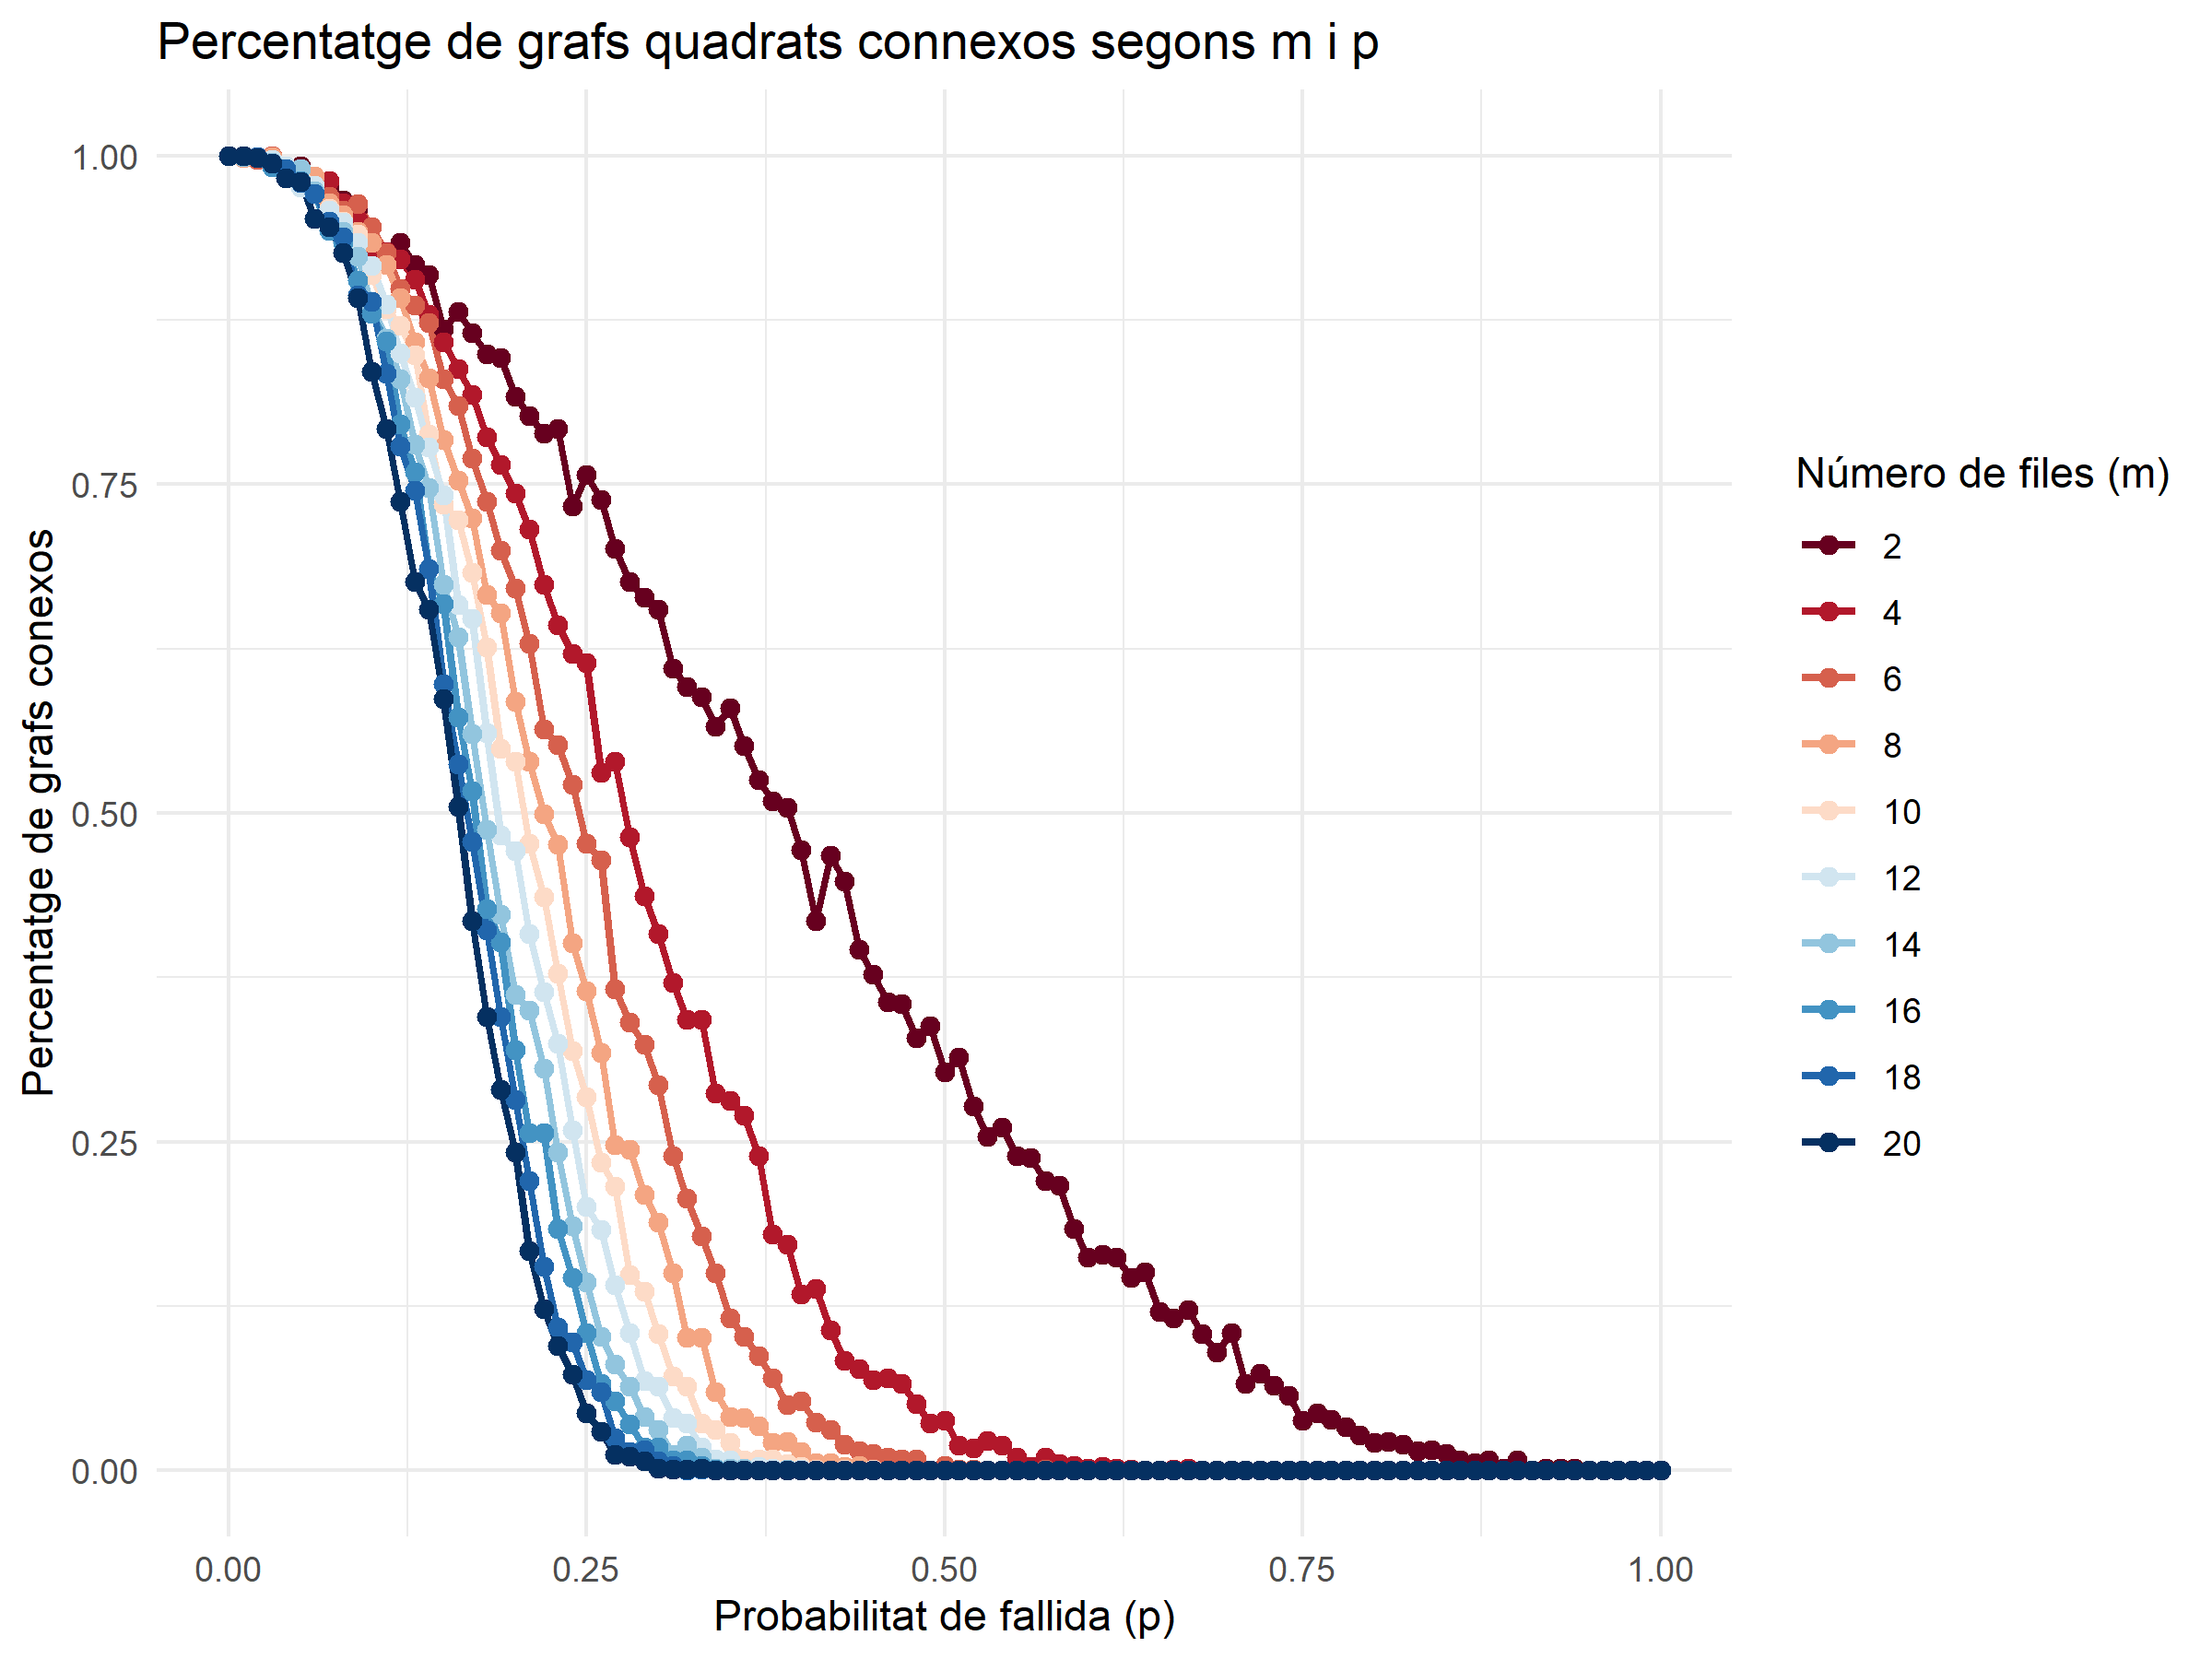
\includegraphics[width=\textwidth]{images/squareE-2-20-1}
			\footnotesize{4321 2 20 2 1000 EDGE\_PERC ./data/squareE-2-20-1.csv Square-Grid}
		\end{minipage}
		\hfill
		\begin{minipage}{0.45\textwidth}
			\centering
			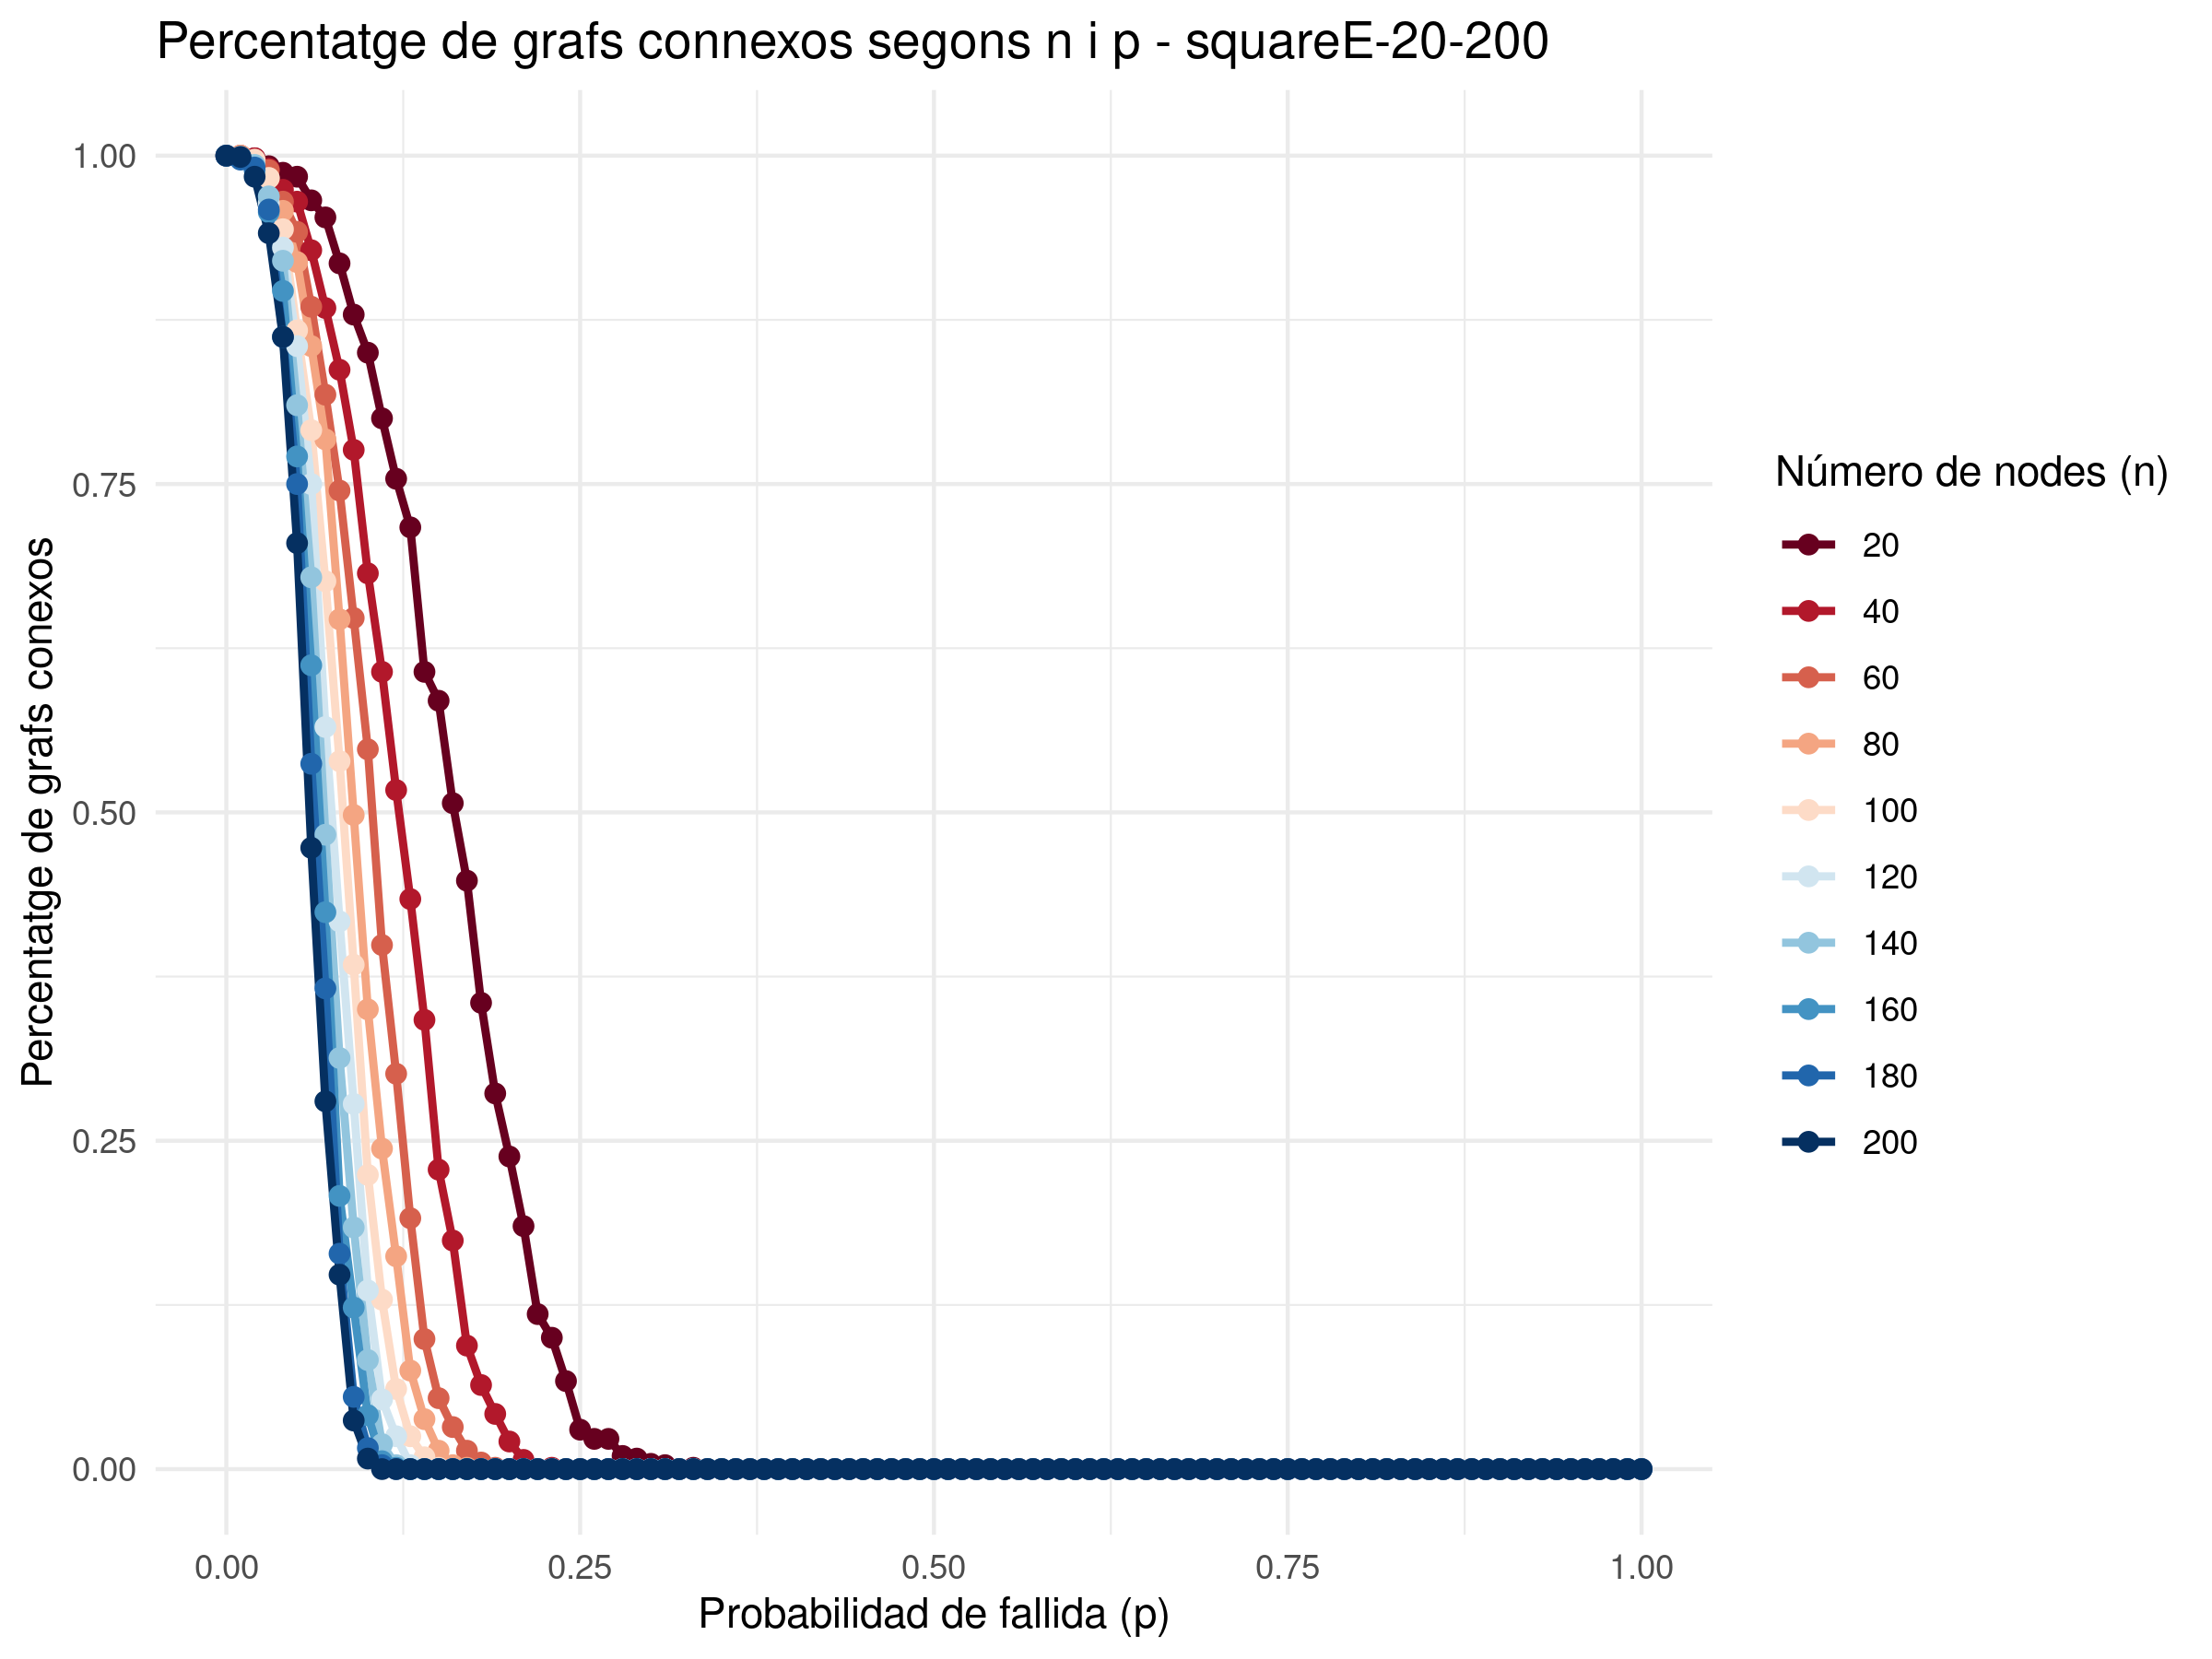
\includegraphics[width=\textwidth]{images/squareE-20-200}
			\footnotesize{4532 20 200 20 1000 EDGE\_PERC ./data/squareE-20-200.csv Square-Grid}
		\end{minipage}
		\caption{Comparativa de percolació per arestes del grafs quadrats amb mides diferents}
		\label{fig:percolation_edges_square}
	\end{figure}
	
	La \textit{Figura \ref{fig:percolation_edges_square}} mostra una comparació de la percolació per arestes en grafs quadrats de mides diferents. Ambdós gràfics representen la relació entre la probabilitat de fallada $p$ (eix x) i el percentatge de grafs connexos (eix y). A mesura que $p$ augmenta, s'eliminen més arestes i, per tant, hi ha menys connectivitat en els grafs resultants. \\
	
	En els dos gràfics, podem veure com a mesura que creix el nombre de nodes dels grafs, la transició de fase s'intensifica i apareix en valors de $p$ més petits. \\
	
	Amb aquests gràfics, podem observar que, tot i que el punt inicial on comença la transició de fase és força similar per a totes les mides de grafs observats, l'abruptesa del canvi de fase és més pronunciada a mesura que $|V|$ augmenta progressivament. A continuació, analitzarem els valors referents al punt \textit{threshold} de cada mida de graf.
	
	\begin{table}[H]
		\centering
		\begin{tabular}{|c|c|c|c|c|c|c|c|c|}
			\hline
			\rowcolor{gray!30}
			M & Threshold & \% Connex & Pendent &   & M & Threshold & \% Connex & Pendent \\ \hline
			2 & 0.24 & 0.73 & -5.90 &   &  20 & 0.17 & 0.42 & -8.70 \\ \hline
			4 & 0.26 & 0.53 & -8.30 &   &  40 & 0.15 & 0.23 & -11.40 \\ \hline
			6 & 0.27 & 0.37 & -9.80 &   &  60 & 0.11 & 0.40 & -14.90 \\ \hline
			8 & 0.24 & 0.40 & -7.50 &   &  80 & 0.09 & 0.50 & -14.90 \\ \hline
			10 & 0.19 & 0.55 & -7.70 &   &  100 & 0.10 & 0.22 & -16.00 \\ \hline
			12 & 0.18 & 0.56 & -8.70 &   &  120 & 0.07 & 0.56 & -18.50 \\ \hline
			14 & 0.17 & 0.56 & -7.40 &   &  140 & 0.07 & 0.48 & -19.60 \\ \hline
			16 & 0.18 & 0.43 & -9.00 &   &  160 & 0.08 & 0.21 & -21.60 \\ \hline
			18 & 0.15 & 0.60 & -8.80 &   &  180 & 0.06 & 0.54 & -21.30 \\ \hline
			20 & 0.17 & 0.42 & -8.70 &   &  200 & 0.06 & 0.47 & -23.20 \\ \hline
		\end{tabular}
		\caption{Dades sobre la transició de fase de grafs quadrats amb percolació per arestes}
		\label{tab:data_edges_square}
	\end{table}
	
	Com hem mencionat anteriorment, la \textit{Taula \ref{tab:data_edges_square}}, ens mostra el $threshold$ on apareix la transició de fase i la probabilitat que el graf sigui connex en aquest valor de $p$, per cada nombre de files del graf. En les graelles de poques files podem veure un $threshold$ que ronda el 0.25, i a mesura que augmenta la mida del graf aquest valor va disminuint. En la taula observem com el threshold disminueix força ràpid al principi, ja que anem augmentant la $M$ de dos en dos i baixa 0.07, mentre que en la segona meitat veiem com disminueix en 0.11 però amb grafs que passen de 20 files a 200. Aixó ens indica que per molt que anem augmentant la mida de la graella el canvi de transició de fase serà cada vegada menor. \\
	
	A més a més, amb la taula podem veure en valors númerics les observacions que feiem amb els gràfics, que el valor de $p$ on hi ha la fallida total disminueix a mesura que la $m$ augmenta i que la transició de fase és més abrupta, ja que observant el pendent que ens indica la taula podem veure que les graelles grans són segments molt més empinats.
	
	\subsubsection{Percolació per nodes}
	
	\begin{figure}[H]
		\centering
		\begin{minipage}{0.45\textwidth}
			\centering
			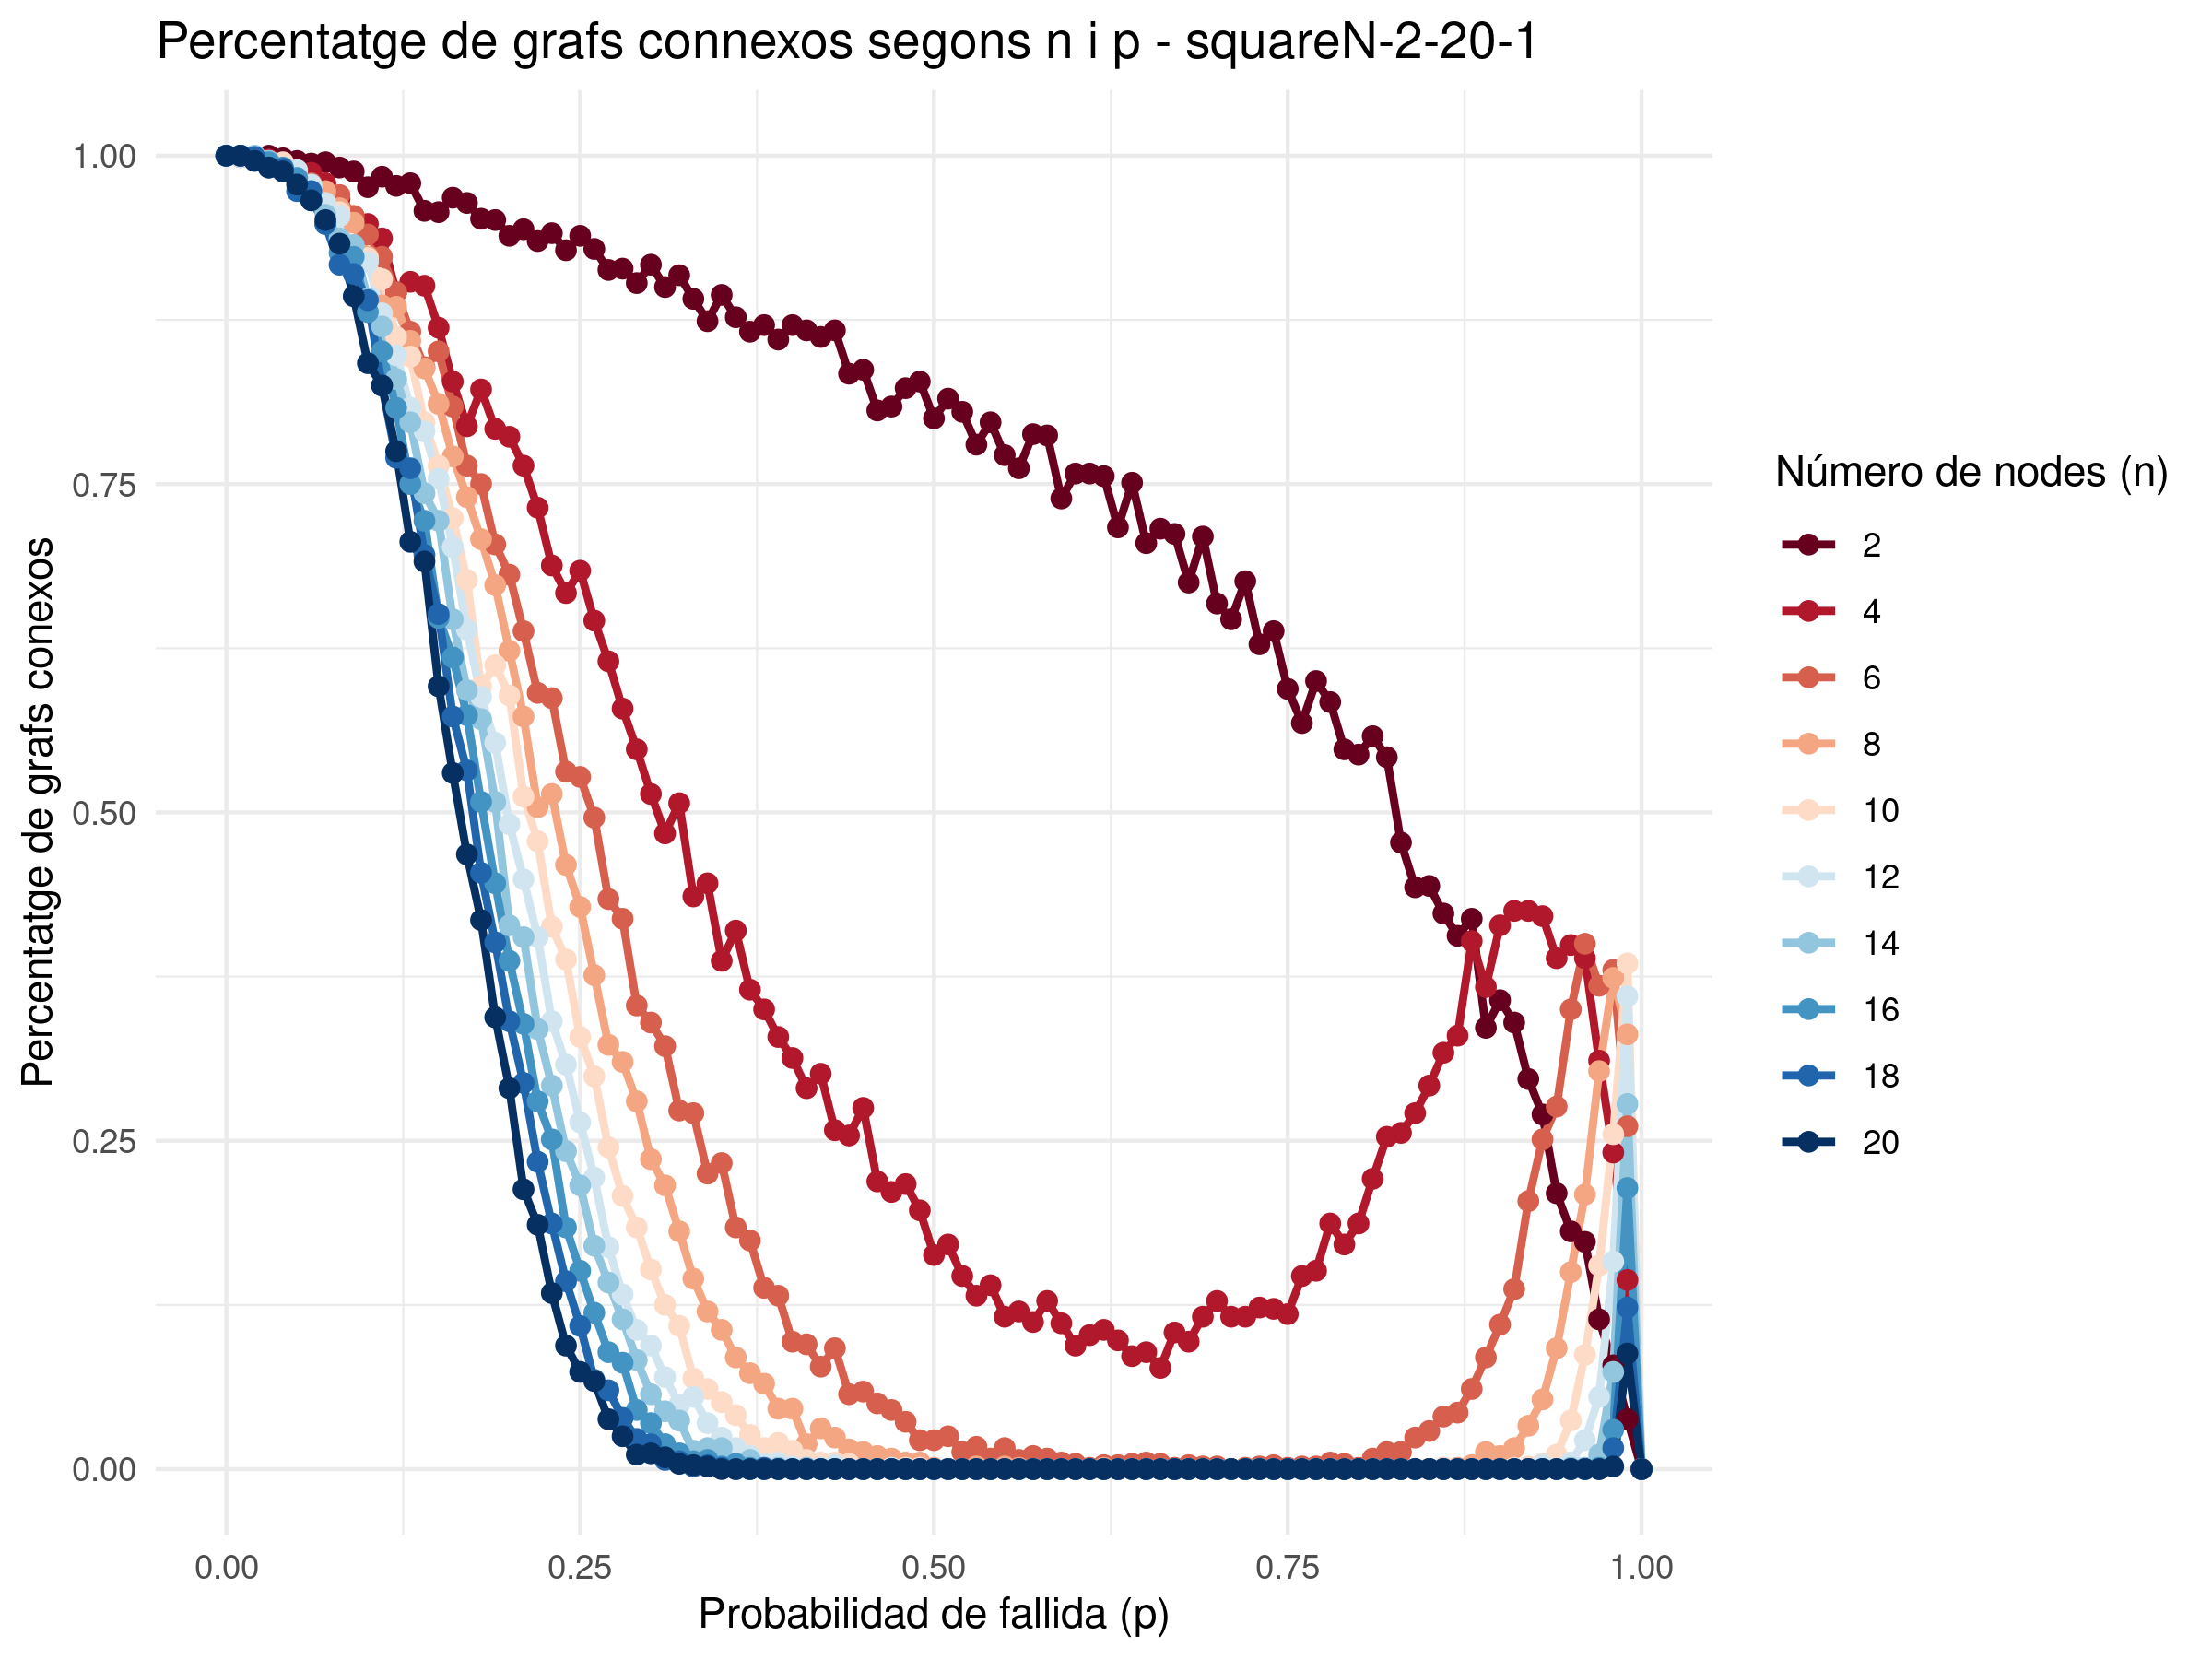
\includegraphics[width=\textwidth]{images/squareN-2-20-1}
			\footnotesize{5202 2 20 2 1000 NODE\_PERC ./data/squareN-2-20-1.csv Square-Grid}
		\end{minipage}
		\hfill
		\begin{minipage}{0.45\textwidth}
			\centering
			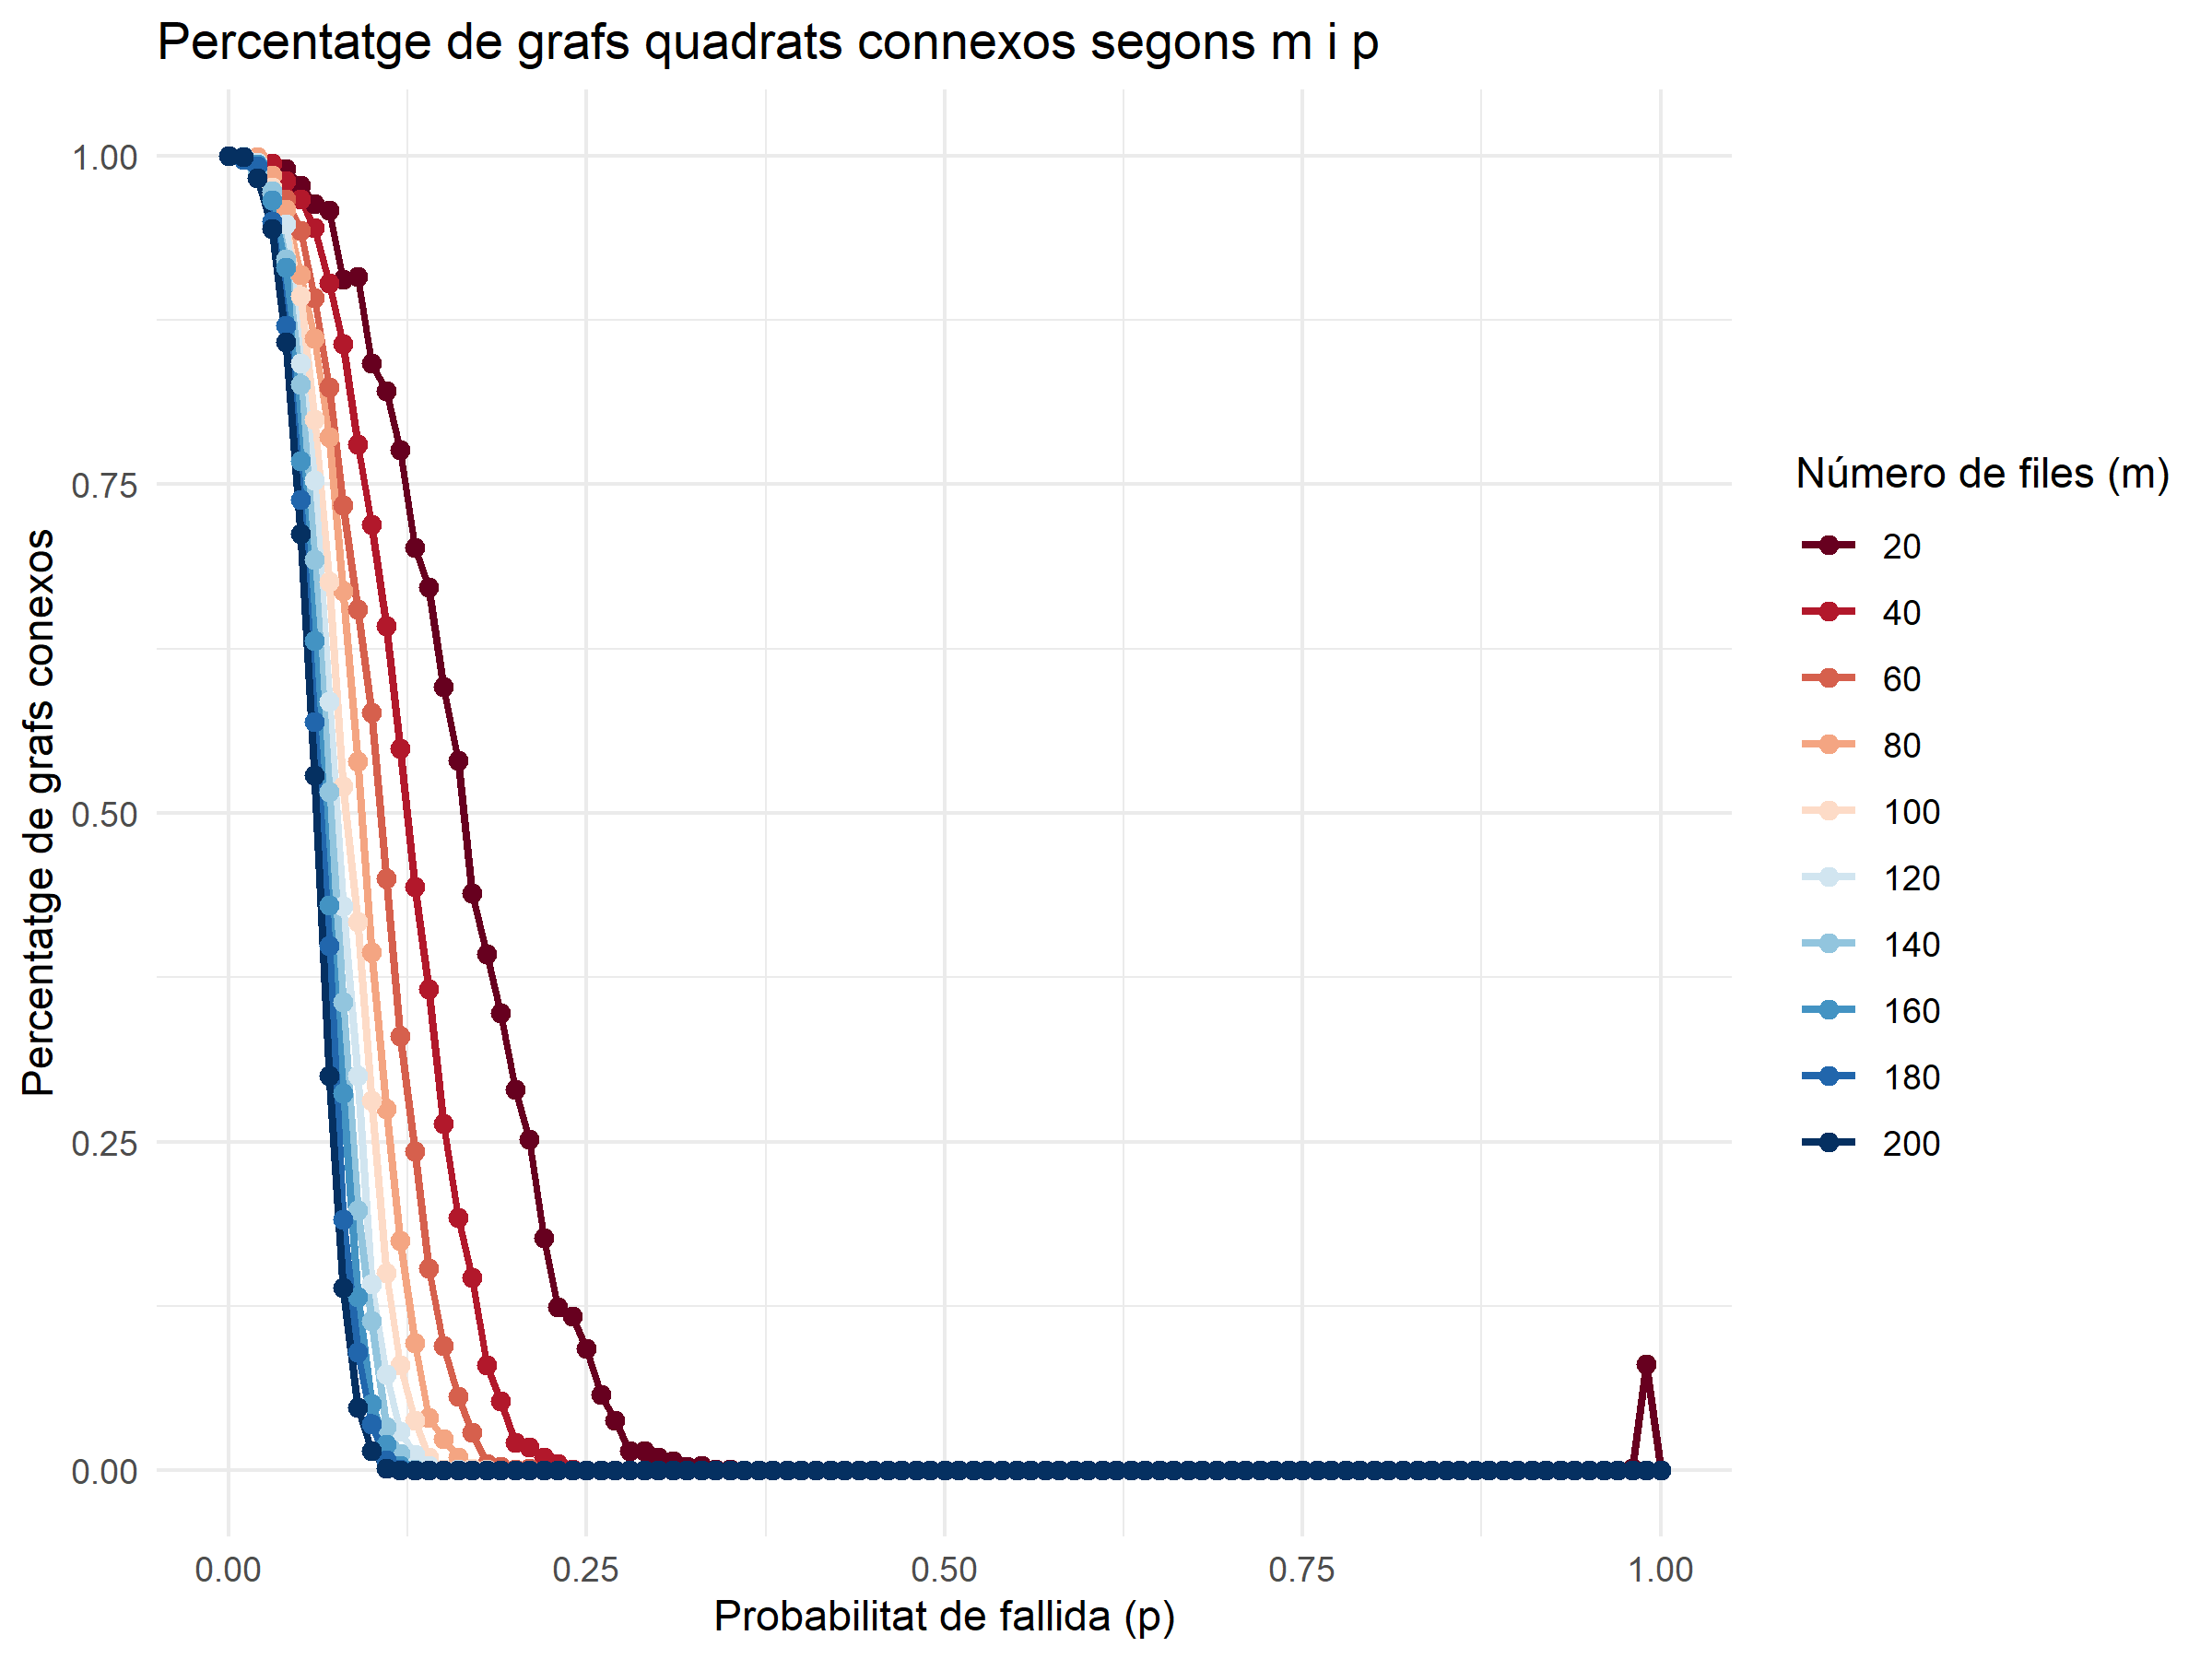
\includegraphics[width=\textwidth]{images/squareN-20-200}
			\footnotesize{4657 20 200 20 1000 NODE\_PERC ./data/squareN-20-200.csv Square-Grid}
		\end{minipage}
		\caption{Comparativa de percolació per nodes del grafs quadrats amb mides diferents}
		\label{fig:percolation_nodes_square}
	\end{figure}
	
	La \textit{Figura \ref{fig:percolation_nodes_square}} mostra la comparació de la percolació per nodes en grafs quadrats de mides diferents. Com en la percolació per arestes, el gràfic de l'esquerra mostra els resultats per grafs petits i el de la dreta grafs més grans. Hem utilitzat les mateixes mides que en la percolació per aresta per poder comparar els resultats i observar diferències en el mètode que utilitzem per percolar. \\
	
	Els resultats representats en el gràfic ens indiquen que graelles quadrades amb molt poques files, menys de 8, continuen mantenint un percentatge alt de connectivitat qualsevol valor de $p$. A mesura que creix la graella aixó es perd i apareix una transició de fase on al arribar a un cert valor de $p$ el graf deixa de ser connex. Igual que en la percolació per arestes, la mida del graf influeix en el pendent de la transició de fase, quan més gran és el graf més ràpida i brusca és la pèrdua de connectivitat. \\
	
	En graelles petites la transició és més suau i fins i tot observem una pujada després de la baixada inicial en valors de $p$ per sobre del 0.75, que indica un increment en el percentatge de grafs connexos quan hi ha una probabilitat de fallida alta. Aquest petit augment final es deu al fet que, amb un valor de $p$ tan alt, s'eliminen molts nodes, i en grafs petits implica que poden apareixer petites components connexes entre elles però aïllades de la resta, cosa que incrementa el percentage de grafs connexos. Aixó no passa en els grafs grans ja que hi ha menys possibilitat que es formin petits \textit{clusters} degut a la distància entre vèrtexs.
	
	
	\subsection{Graella triangular}
	
	Ara estudiem la transició de fase en graelles triangulars. En aquest cas només havíem d'estudiar la percolació per aresta i ho hem fet com en les graelles quadrades, amb grafs de mida petita i mida més gran. En aquest cas, els grafs petits comencen amb 5 files fins a 55 files, amb increment de 5 files cada vegada, mentre que la mida gran son grafs de 50 a 150 files amb increments de 10 files. \\
	
	Hem decidit fer la percolació per aresta perquè volíem veure si el fet de tenir una graella similar a la graella quadrada, pero amb els vertex del mig (els que no estan a la vora del graf i per tant tenen totes les arestes possibles) de grau més alt influiria en el valor de la probabilitat de fallida on hi ha la transició de fase. Creiem que en aquest cas la probabilitat de fallida on hi ha la transició de fase serà un valor més alt que en graelles quadrades ja que el grau dels vèrtex és més alt i per tant hi ha més arestes que han de fallar per desconnectar els nodes. Després de fer aquesta experimentació, hem decidit fer també l'estudi per percolació de node per poder comparar els resultats amb els obtinguts en graelles quadrades. \\
	
	
	\subsubsection{Percolació per aresta}
	
	\begin{figure}[H]
		\centering
		\begin{minipage}{0.45\textwidth}
			\centering
			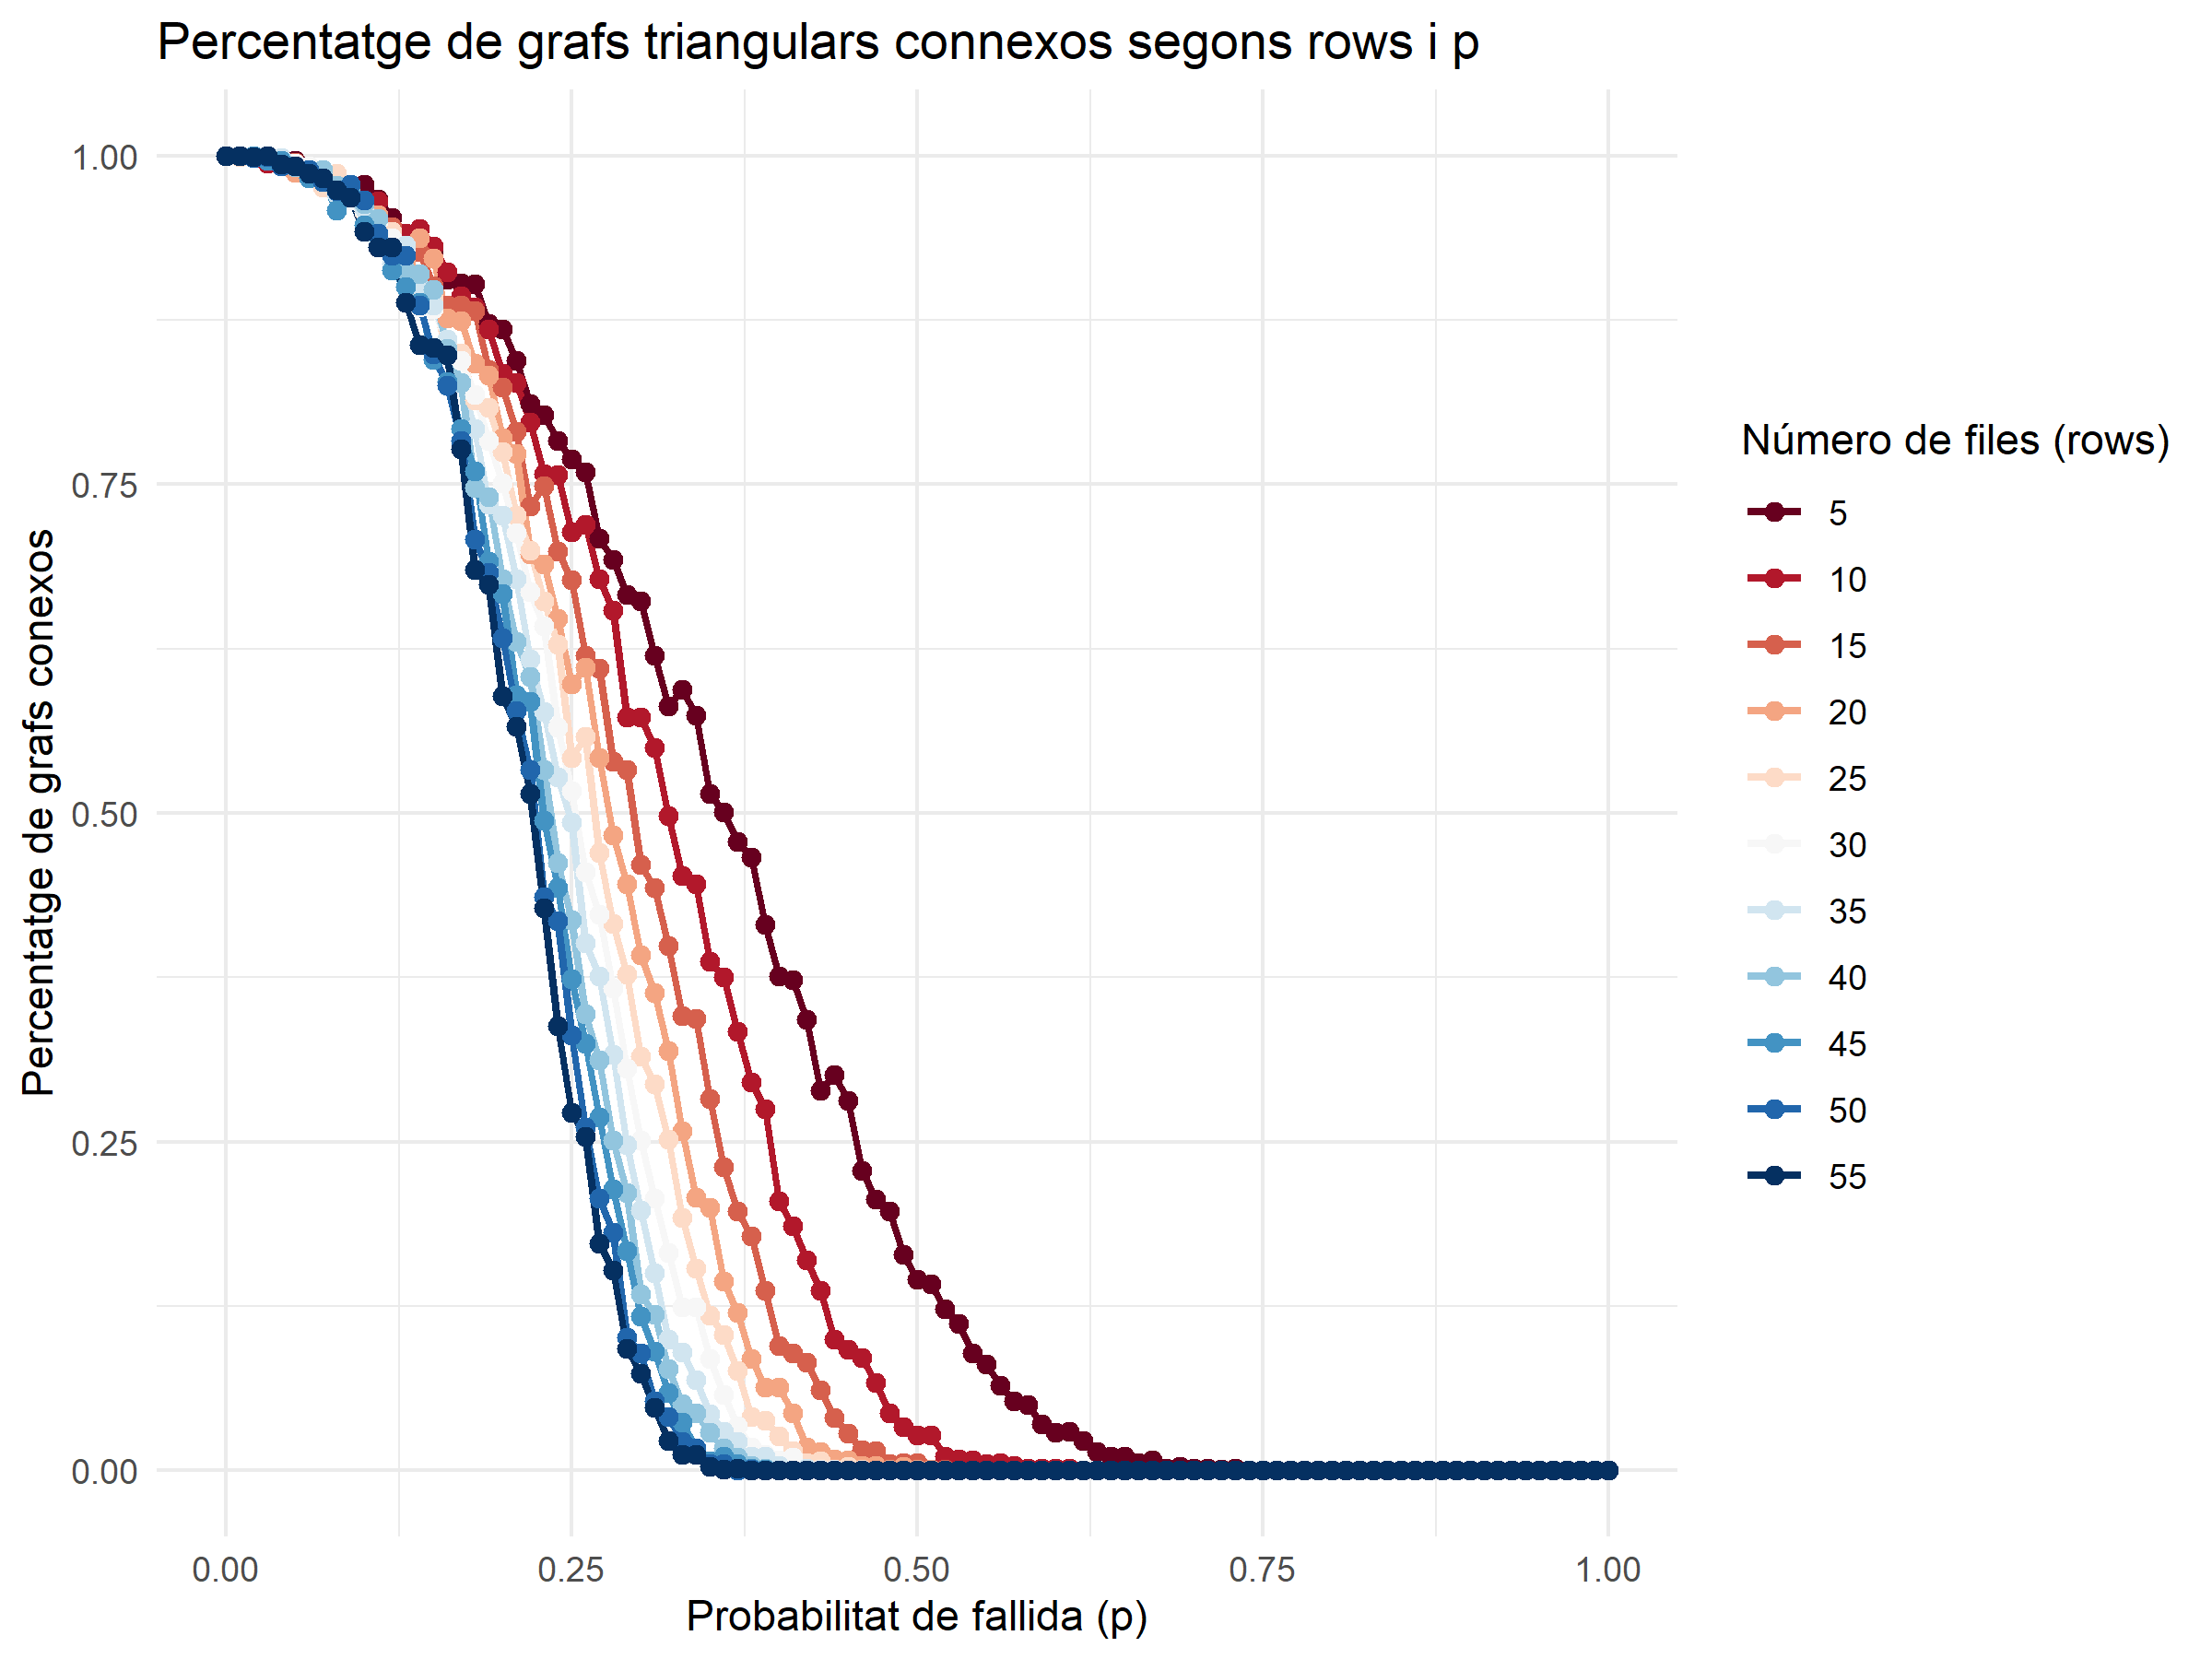
\includegraphics[width=\textwidth]{images/triangularE-5-55-1000}
			\footnotesize{3497 5 55 5 1000 EDGE\_PERC ./data/triangularE-5-55-1000.csv Triangular-Grid}
		\end{minipage}
		\hfill
		\begin{minipage}{0.45\textwidth}
			\centering
			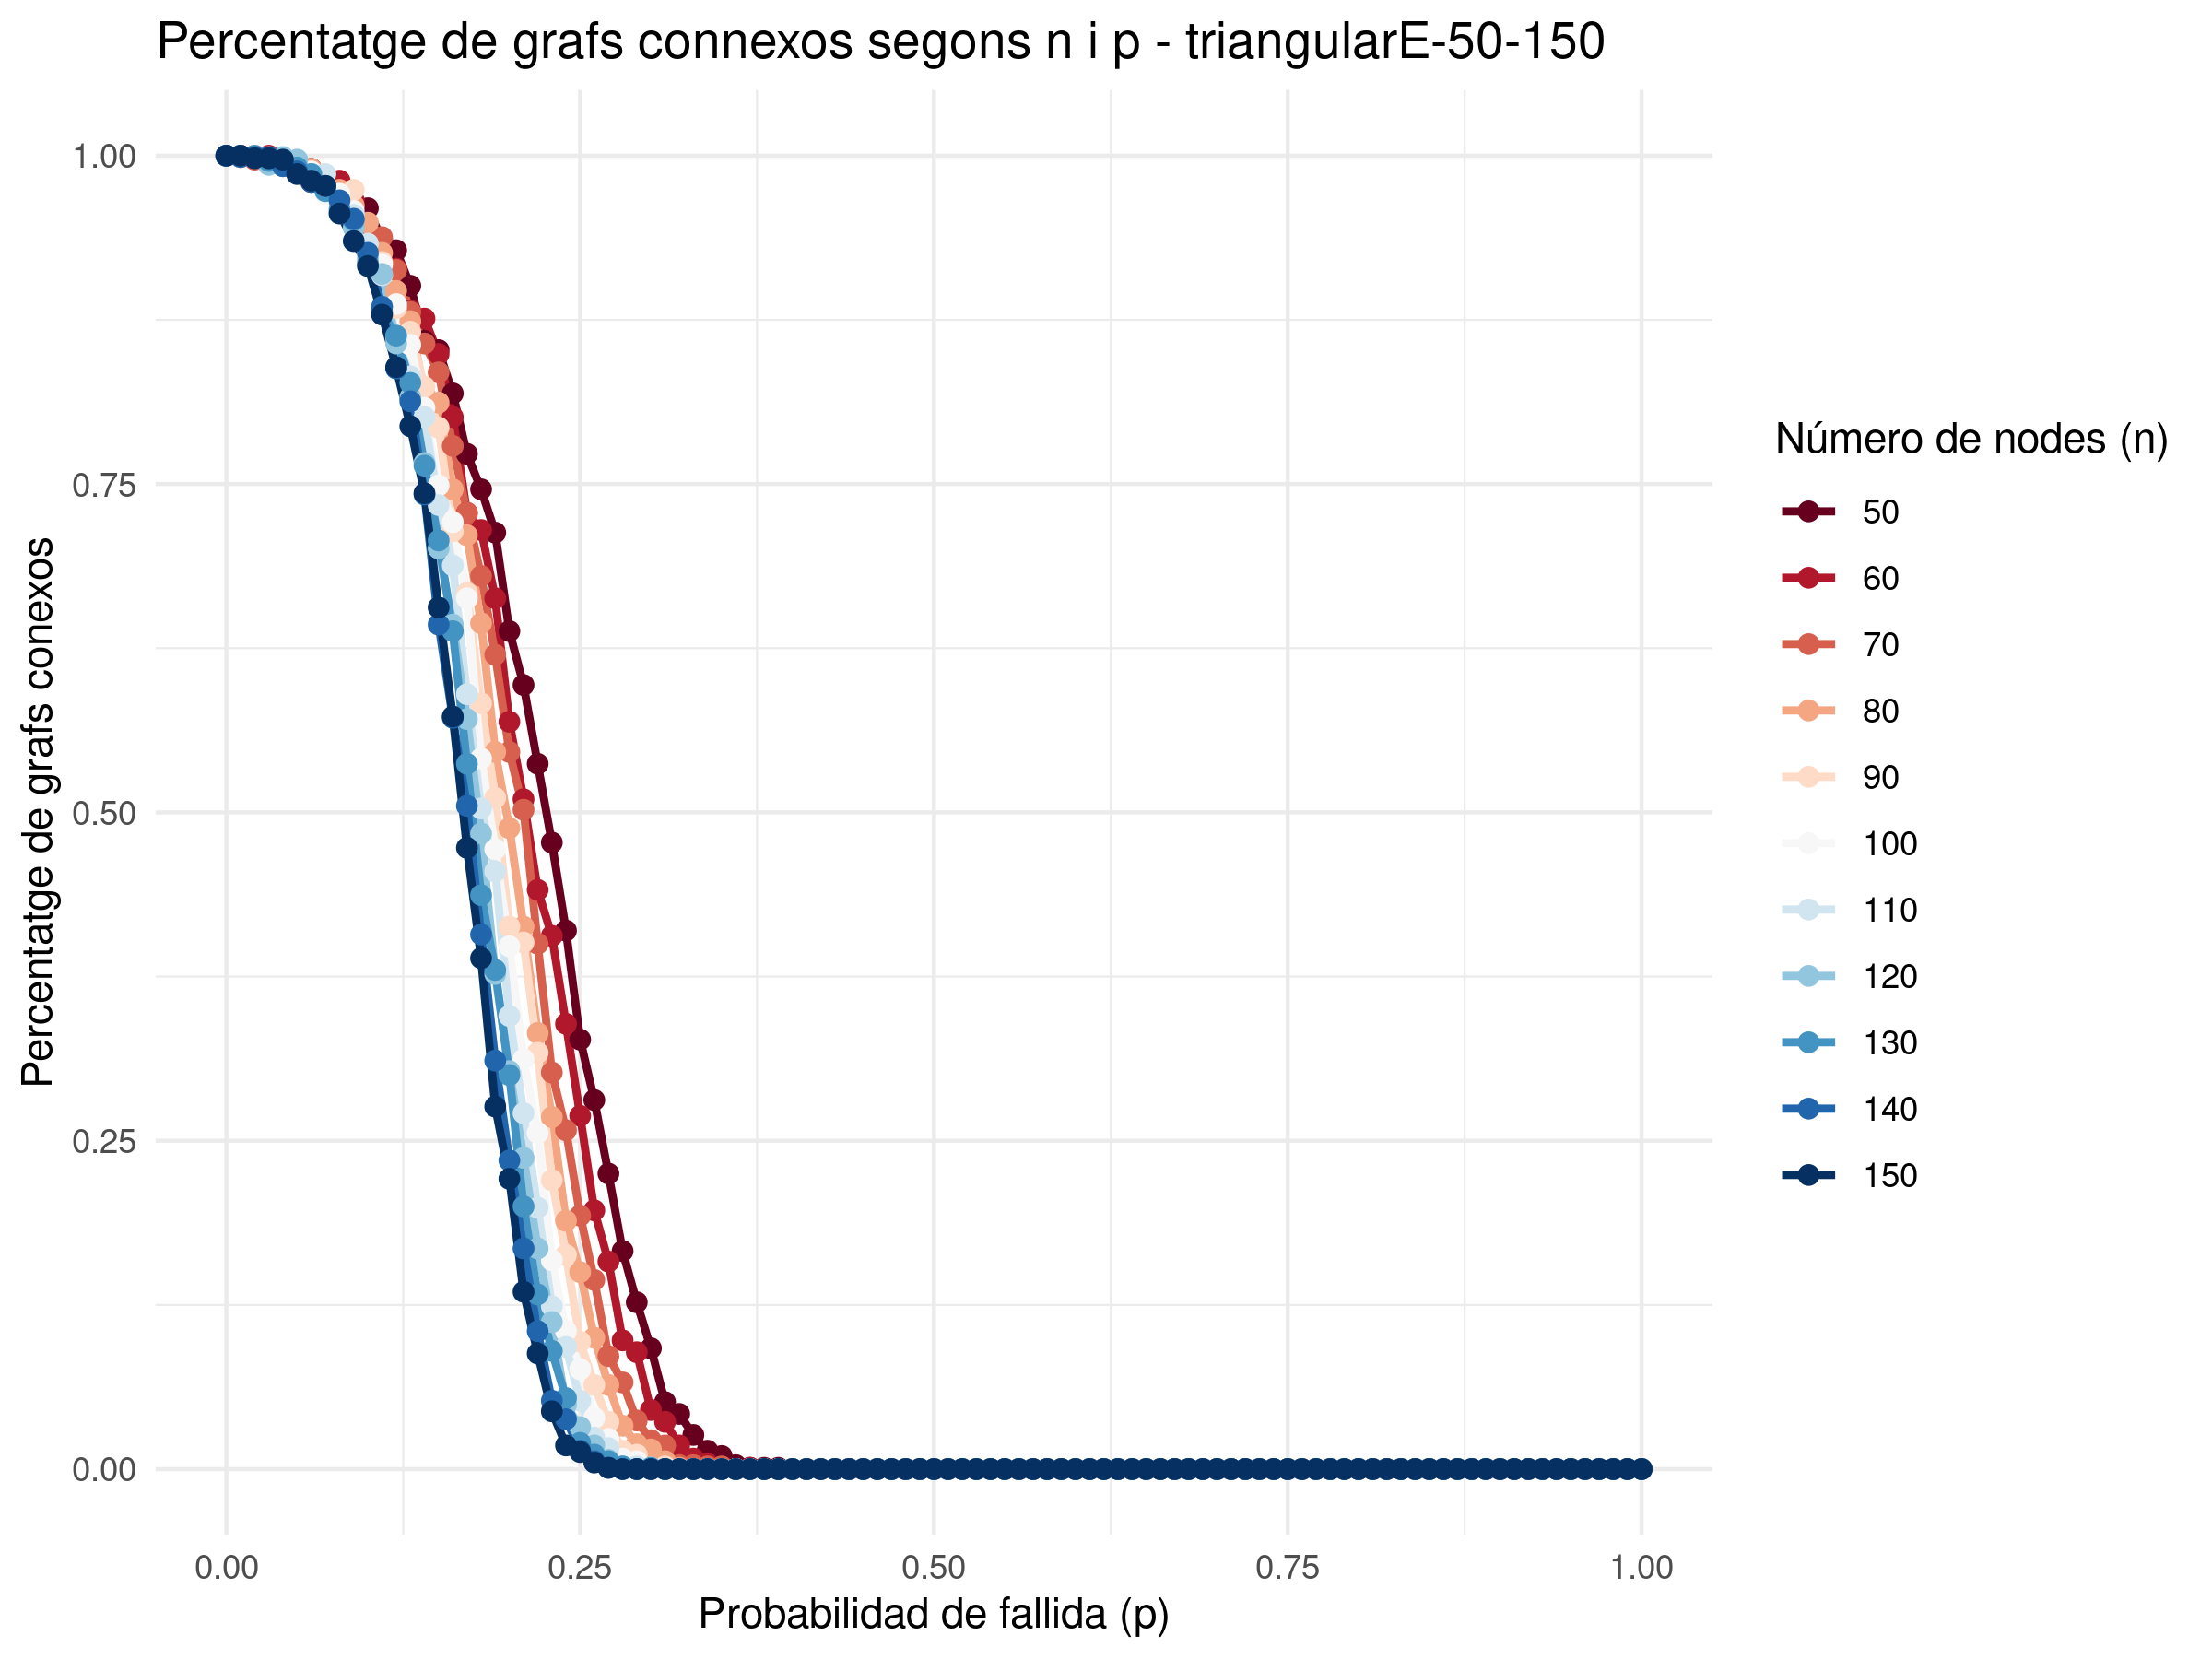
\includegraphics[width=\textwidth]{images/triangularE-50-150}
			\footnotesize{3363 50 150 10 1000 EDGE\_PERC ./data/triangularE-50-150.csv Triangular-Grid}
		\end{minipage}
		\caption{Comparativa de percolació per arestes de graelles triangulars amb mides diferents}
		\label{fig:percolation_edges_triangular}
	\end{figure}
	
	La \textit{Figura \ref{fig:percolation_edges_triangular}} mostra la comparació de percolació per arestes de graelles triangulars amb els resultats dels grafs petits a l'esquerra i els grans al gràfic de la dreta. La informació que cada gràfic proporciona és la mateixa que en l'experimentació de les graelles quadrades, cada línea indica la relació entre percentatge de grafs connexos i probabilitat de fallida \textit{p} en funció del número de files. \\
	
	En els dos casos podem observar que hi ha una transició de fase ja que hi ha una caiguda brusca en un valor determinat de \textit{p}, però en el cas dels grafs petits aquesta caiguda és més gradual, la transició de fase no està tant marcada. En canvi, en grafs amb més files la transició és més ràpida i, si ens fixem en el valor de la probabilitat de fallida on arribem a la desconnexió total, la \textit{p} que marca la transició de fase disminueix a mesura que el graf és més gran. \\
	
	Per tant, igual que en els grafs quadrats la mida del graf afecta el valor de la probabilitat de fallida on ocorre la transició de fase, la qual disminueix a mesura que el graf augmenta de mida. 
	
	\begin{table}[H]
		\centering
		\begin{tabular}{|c|c|c|c|c|c|c|c|c|}
			\hline
			\rowcolor{gray!30}
			M & Threshold & \% Connex & Pendent &   & M & Threshold & \% Connex & Pendent \\ \hline
			5 & 0.35 & 0.52 & -5.90  &   & 50 & 0.25 & 0.33 & -8.30 \\ \hline
			10 & 0.29 & 0.57 & -8.10 &   & 60 & 0.20 & 0.57 & -9.40 \\ \hline
			15 & 0.30 & 0.46 & -7.20 &   & 70 & 0.22 & 0.40 & -10.20 \\ \hline
			20 & 0.22 & 0.70 & -7.60 &   & 80 & 0.19 & 0.55 & -9.80 \\ \hline
			25 & 0.27 & 0.47 & -8.80 &   & 90 & 0.20 & 0.41 & -9.80 \\ \hline
			30 & 0.24 & 0.56 & -7.70 &   & 100 & 0.18 & 0.54 & -12.20 \\ \hline
			35 & 0.26 & 0.40 & -9.20 &   & 110 & 0.20 & 0.34 & -11.00 \\ \hline
			40 & 0.18 & 0.75 & -8.00 &   & 120 & 0.19 & 0.38 & -10.70 \\ \hline
			45 & 0.23 & 0.49 & -9.10 &   & 130 & 0.17 & 0.54 & -10.10 \\ \hline
			50 & 0.23 & 0.44 & -9.70 &   & 140 & 0.15 & 0.64 & -9.90 \\ \hline
			55 & 0.18 & 0.68 & -9.20 &   & 150 & 0.19 & 0.28 & -11.30 \\ \hline
			
		\end{tabular}
		\caption{Dades sobre la transició de fase de grafs triangulars amb percolació per arestes}
		\label{tab:data_edges_triangulars}
	\end{table}
	
	Amb la \textit{Taula \ref{tab:data_edges_triangulars}}, observem númericament el que hem explicat dels gràfics, que el valor on hi ha la transició de fase va disminuint a mesura que $M$ augmenta. Igual que en les graelles quadrades, cada vegada disminueix més a poc a poc el $threshold$, però per contra incrementa el pendent en el punt \textit{threshold}. Aixó ens indica que la pèrdua de connectivitat és més abrupta en grafs més grans i que la transició de fase es influenciada per la mida del graf. \\
	
	Pel que fa a la comparació que ens interessava amb les graelles quadrades, tot i que observant els gràfics ja es pot veure que la $p$ on hi ha la desconnexió total és més petita en les graelles quadrades, en aquesta taula podem observar resultats de grafs amb el mateix número de files per poder veure millor la comparació.
	
	\begin{table}[H]
		\centering
		\begin{tabular}{|c|c|c|}
			\hline
			\rowcolor{gray!30}
			\# files & $\textit{Threshold}\texttt{ square}$ &$\textit{Threshold}\texttt{ triangular}$ \\ \hline
			10 & 0.19 & 0.29 \\ \hline
			20 & 0.17 & 0.22 \\ \hline
			40 & 0.15 & 0.18 \\ \hline
			60 & 0.11 & 0.20 \\ \hline
			80 & 0.09 & 0.19 \\ \hline
			100 & 0.10 & 0.18\\ \hline
			120 & 0.07 & 0.19 \\ \hline
			140 & 0.07 & 0.15 \\ \hline
		\end{tabular}
		\caption{Comparació del punt \textit{threshold} entre els grafs quadrats i triangulars amb percolació per arestes}
		\label{tab:comparacio_threshold_square_triangular_edges}
	\end{table}
	
	La \textit{Taula \ref{tab:comparacio_threshold_square_triangular_edges}} ens mostra una comparació de $threshold$ en grafs amb el mateix nombre de files però de diferent tipus, graelles quadrades o triangulars. Com ja hem anat suposant però amb la taula podem confirmar, en les graelles quadrades el moment on apareix la transició de fase és més petit que en les graelles triangulars. Amb aquestes dades podem confirmar la nostra hipòtesi d'experimentació on crèiem que el fet de tenir graelles on els nodes tenen més arestes influiria en el valor $p$ on apareix la transició de fase.
	
	\subsubsection{Percolació per node}
	
	\begin{figure}[H]
		\centering
		\begin{minipage}{0.45\textwidth}
			\centering
			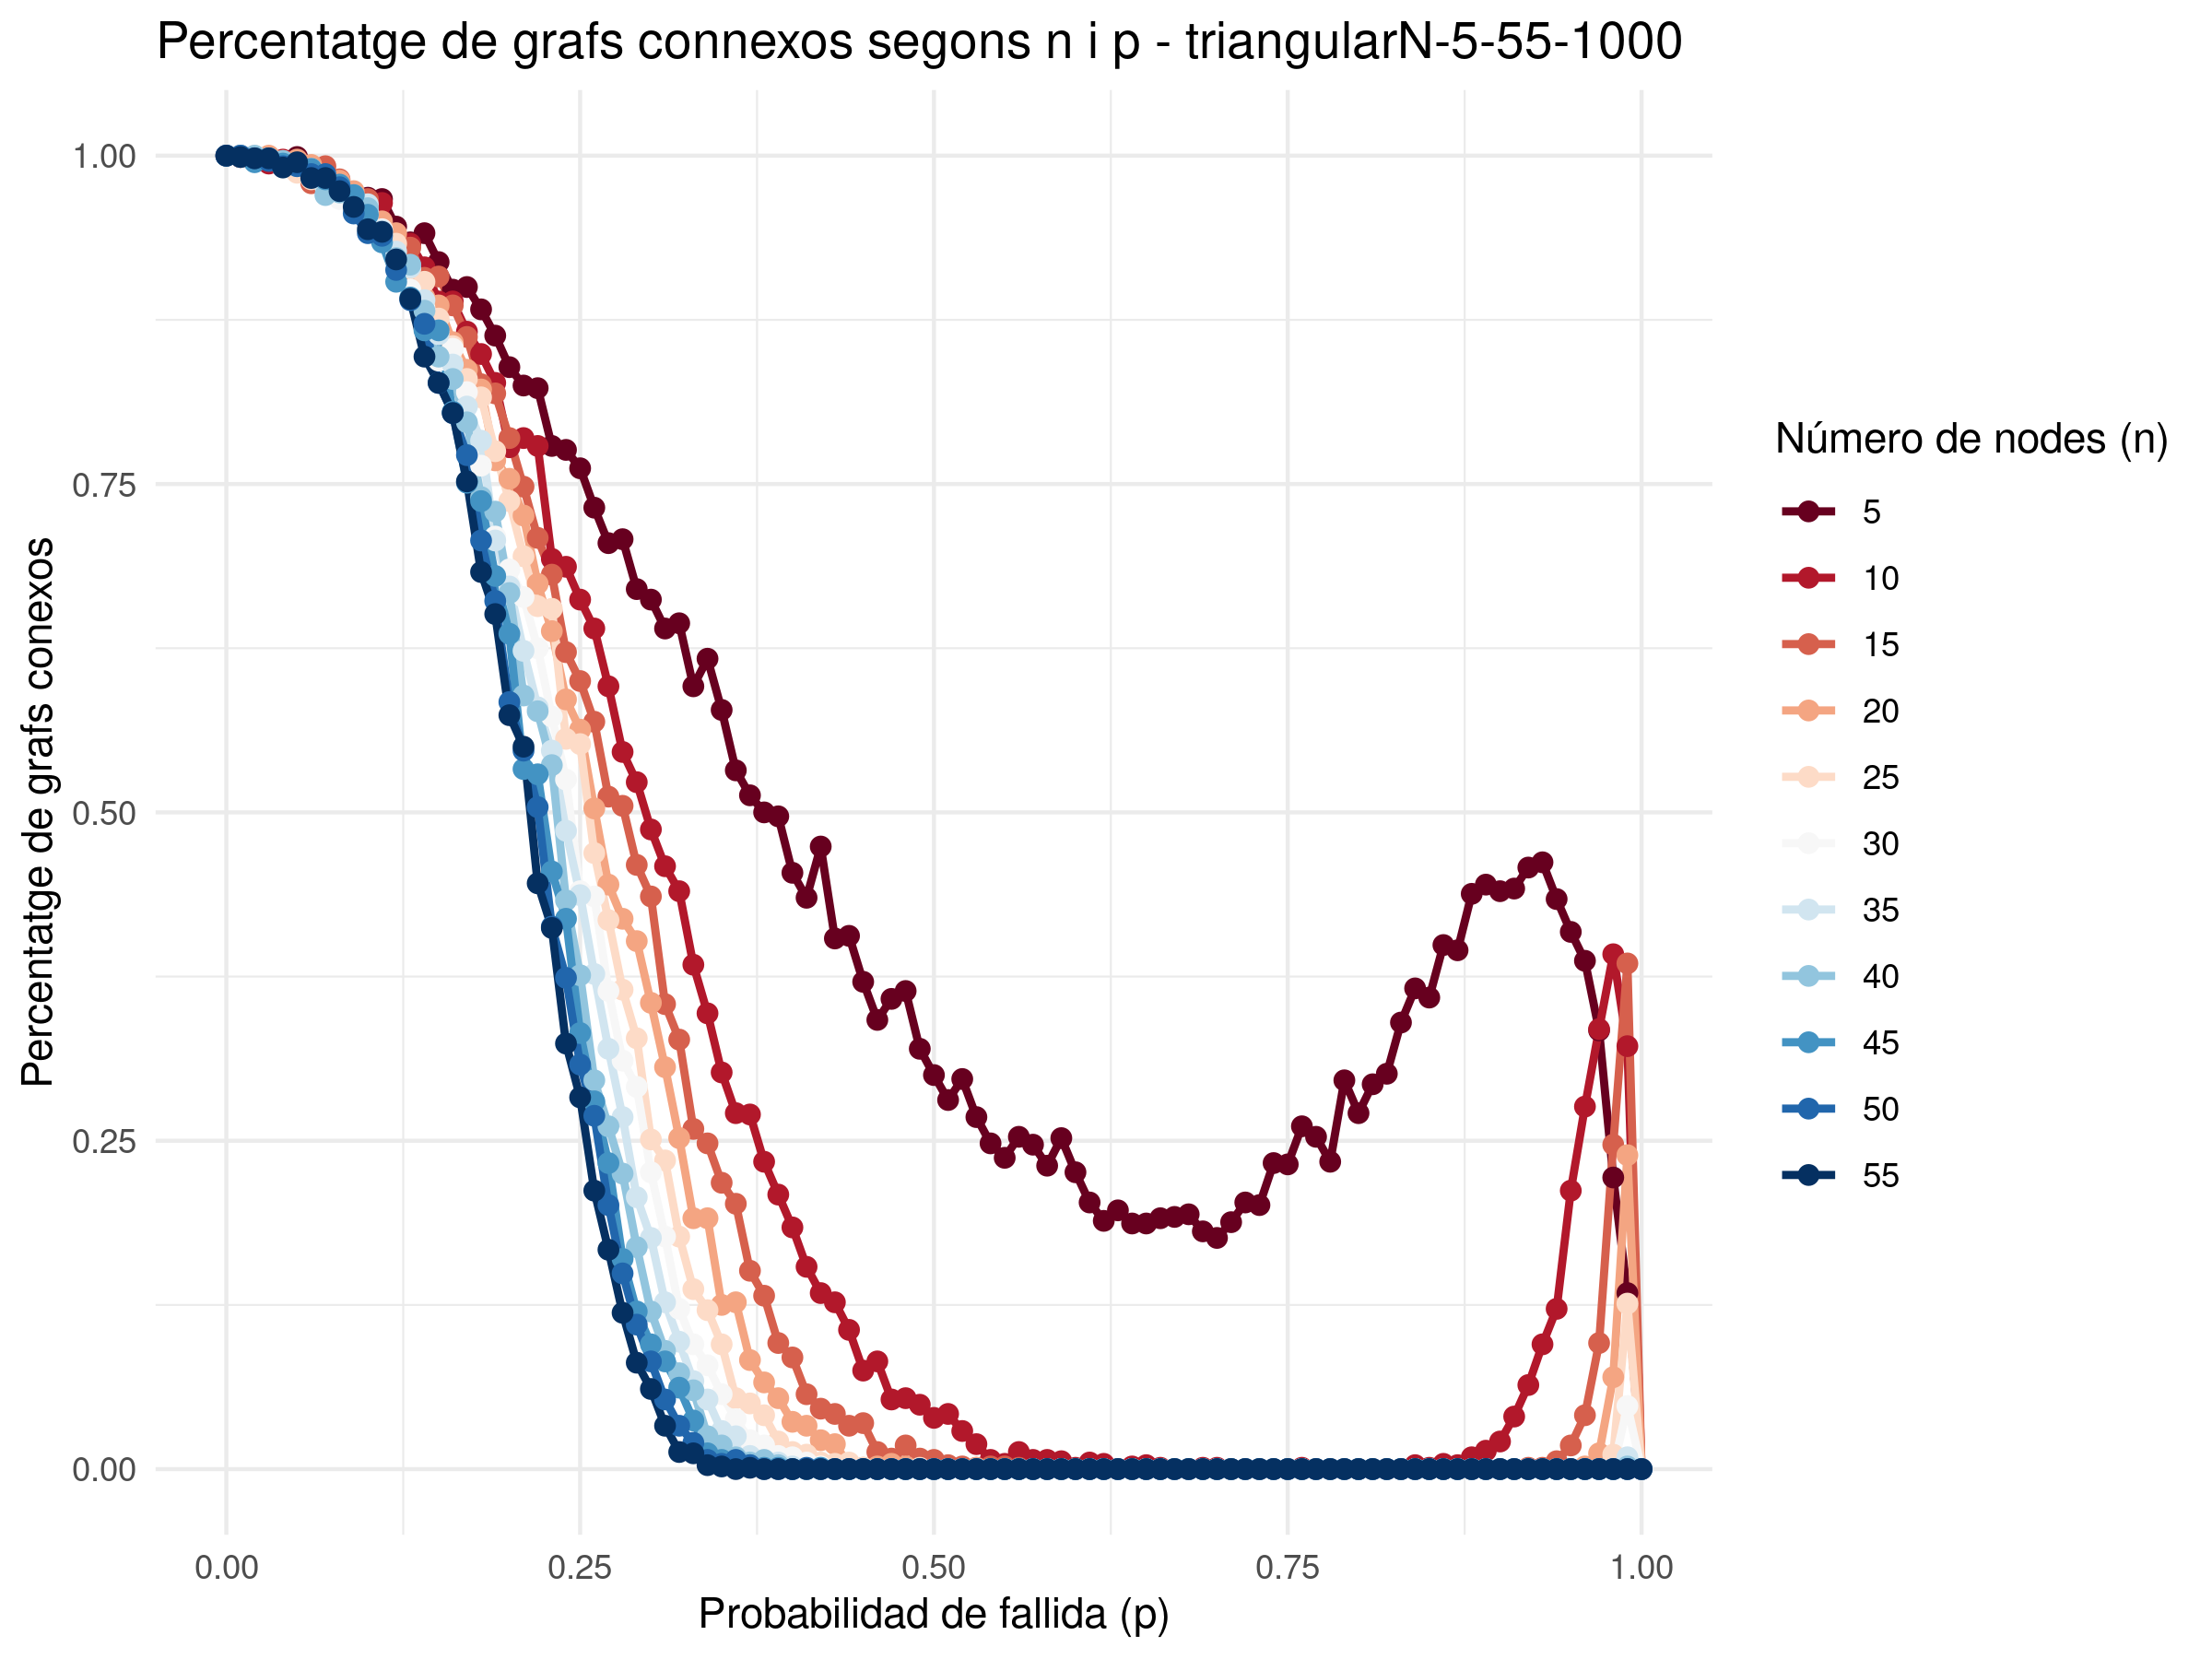
\includegraphics[width=\textwidth]{images/triangularN-5-55-1000}
			\footnotesize{7002 5 55 5 1000 NODE\_PERC ./data/triangularN-5-55-1000.csv Triangular-Grid}
		\end{minipage}
		\hfill
		\begin{minipage}{0.45\textwidth}
			\centering
			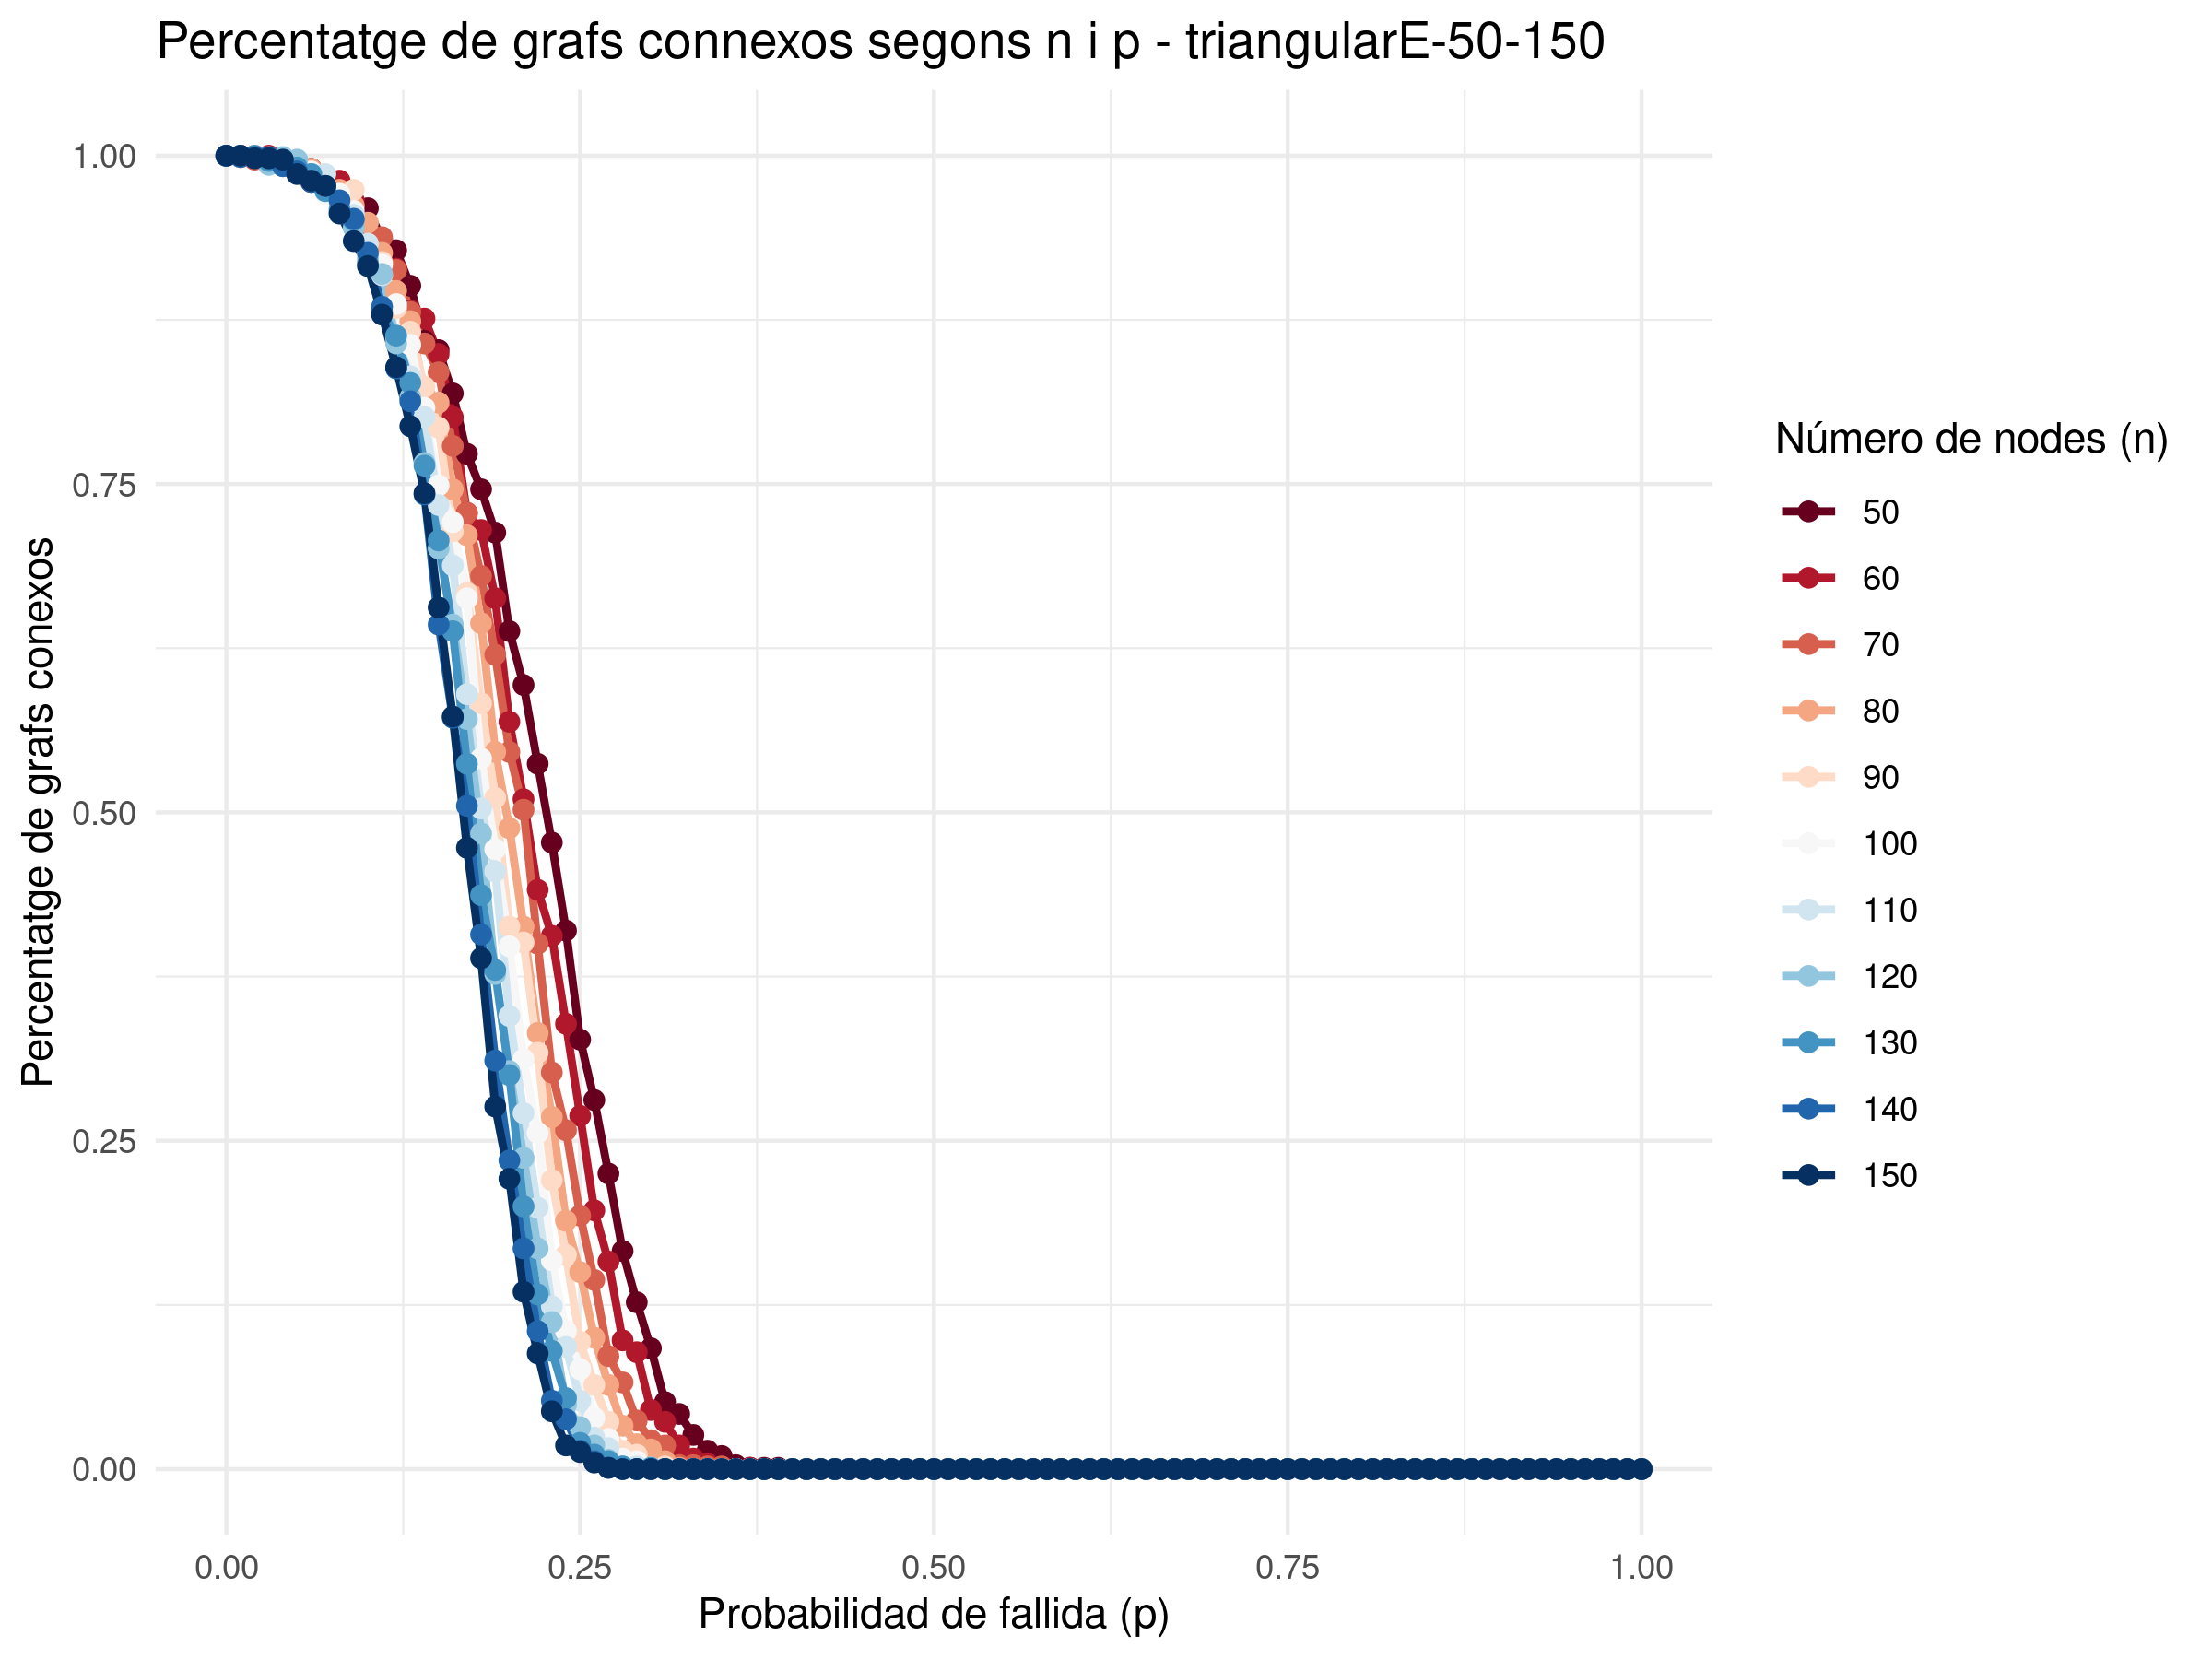
\includegraphics[width=\textwidth]{images/triangularE-50-150}
			\footnotesize{4056 50 150 10 1000 NODE\_PERC ./data/triangularN-50-150.csv Triangular-Grid}
		\end{minipage}
		\caption{Comparativa de percolació per nodes de graelles triangulars amb mides diferents}
		\label{fig:percolation_nodes_triangular}
	\end{figure}
	
	
	\subsection{Graf geomètric aleatori}
	
	L'estudi de transició sobre grafs geometrics aleatoris depèn, a més de la probabilitat de percolació $p$, dels dos paràmetres que s'utilitzen per a la creació del graf: el nombre de nodes $n$ i el radi de connectivitat $r$.
	En aquesta experimentació, s'han fet 6 casos de prova, on es compara l'impacte de tots dos paràmetres en diferents nivells. En el cas del nombre de nodes $n$, els valors que s'han utilitzar són de 10 a 100 i de 100 a 1000,
	donant-nos resultats per a grafs amb pocs nodes fins a grafs amb una quantitat relativament gran de nodes. Per part del radi de connectivitat $r$, els valors que s'han escollit són de 0.2, 0.5, 0.8, que ens permeten observar grafs amb una connectivitat
	bastant feble en el cas del primer valor, grafs amb una connectivitat molt alta amb $r$ = 0.8 i un mig entre tots dos valors.
	
	\subsubsection{Percolació per arestes}
	
	\begin{figure}[H]
		\centering
		\begin{minipage}{0.45\textwidth}
			\centering
			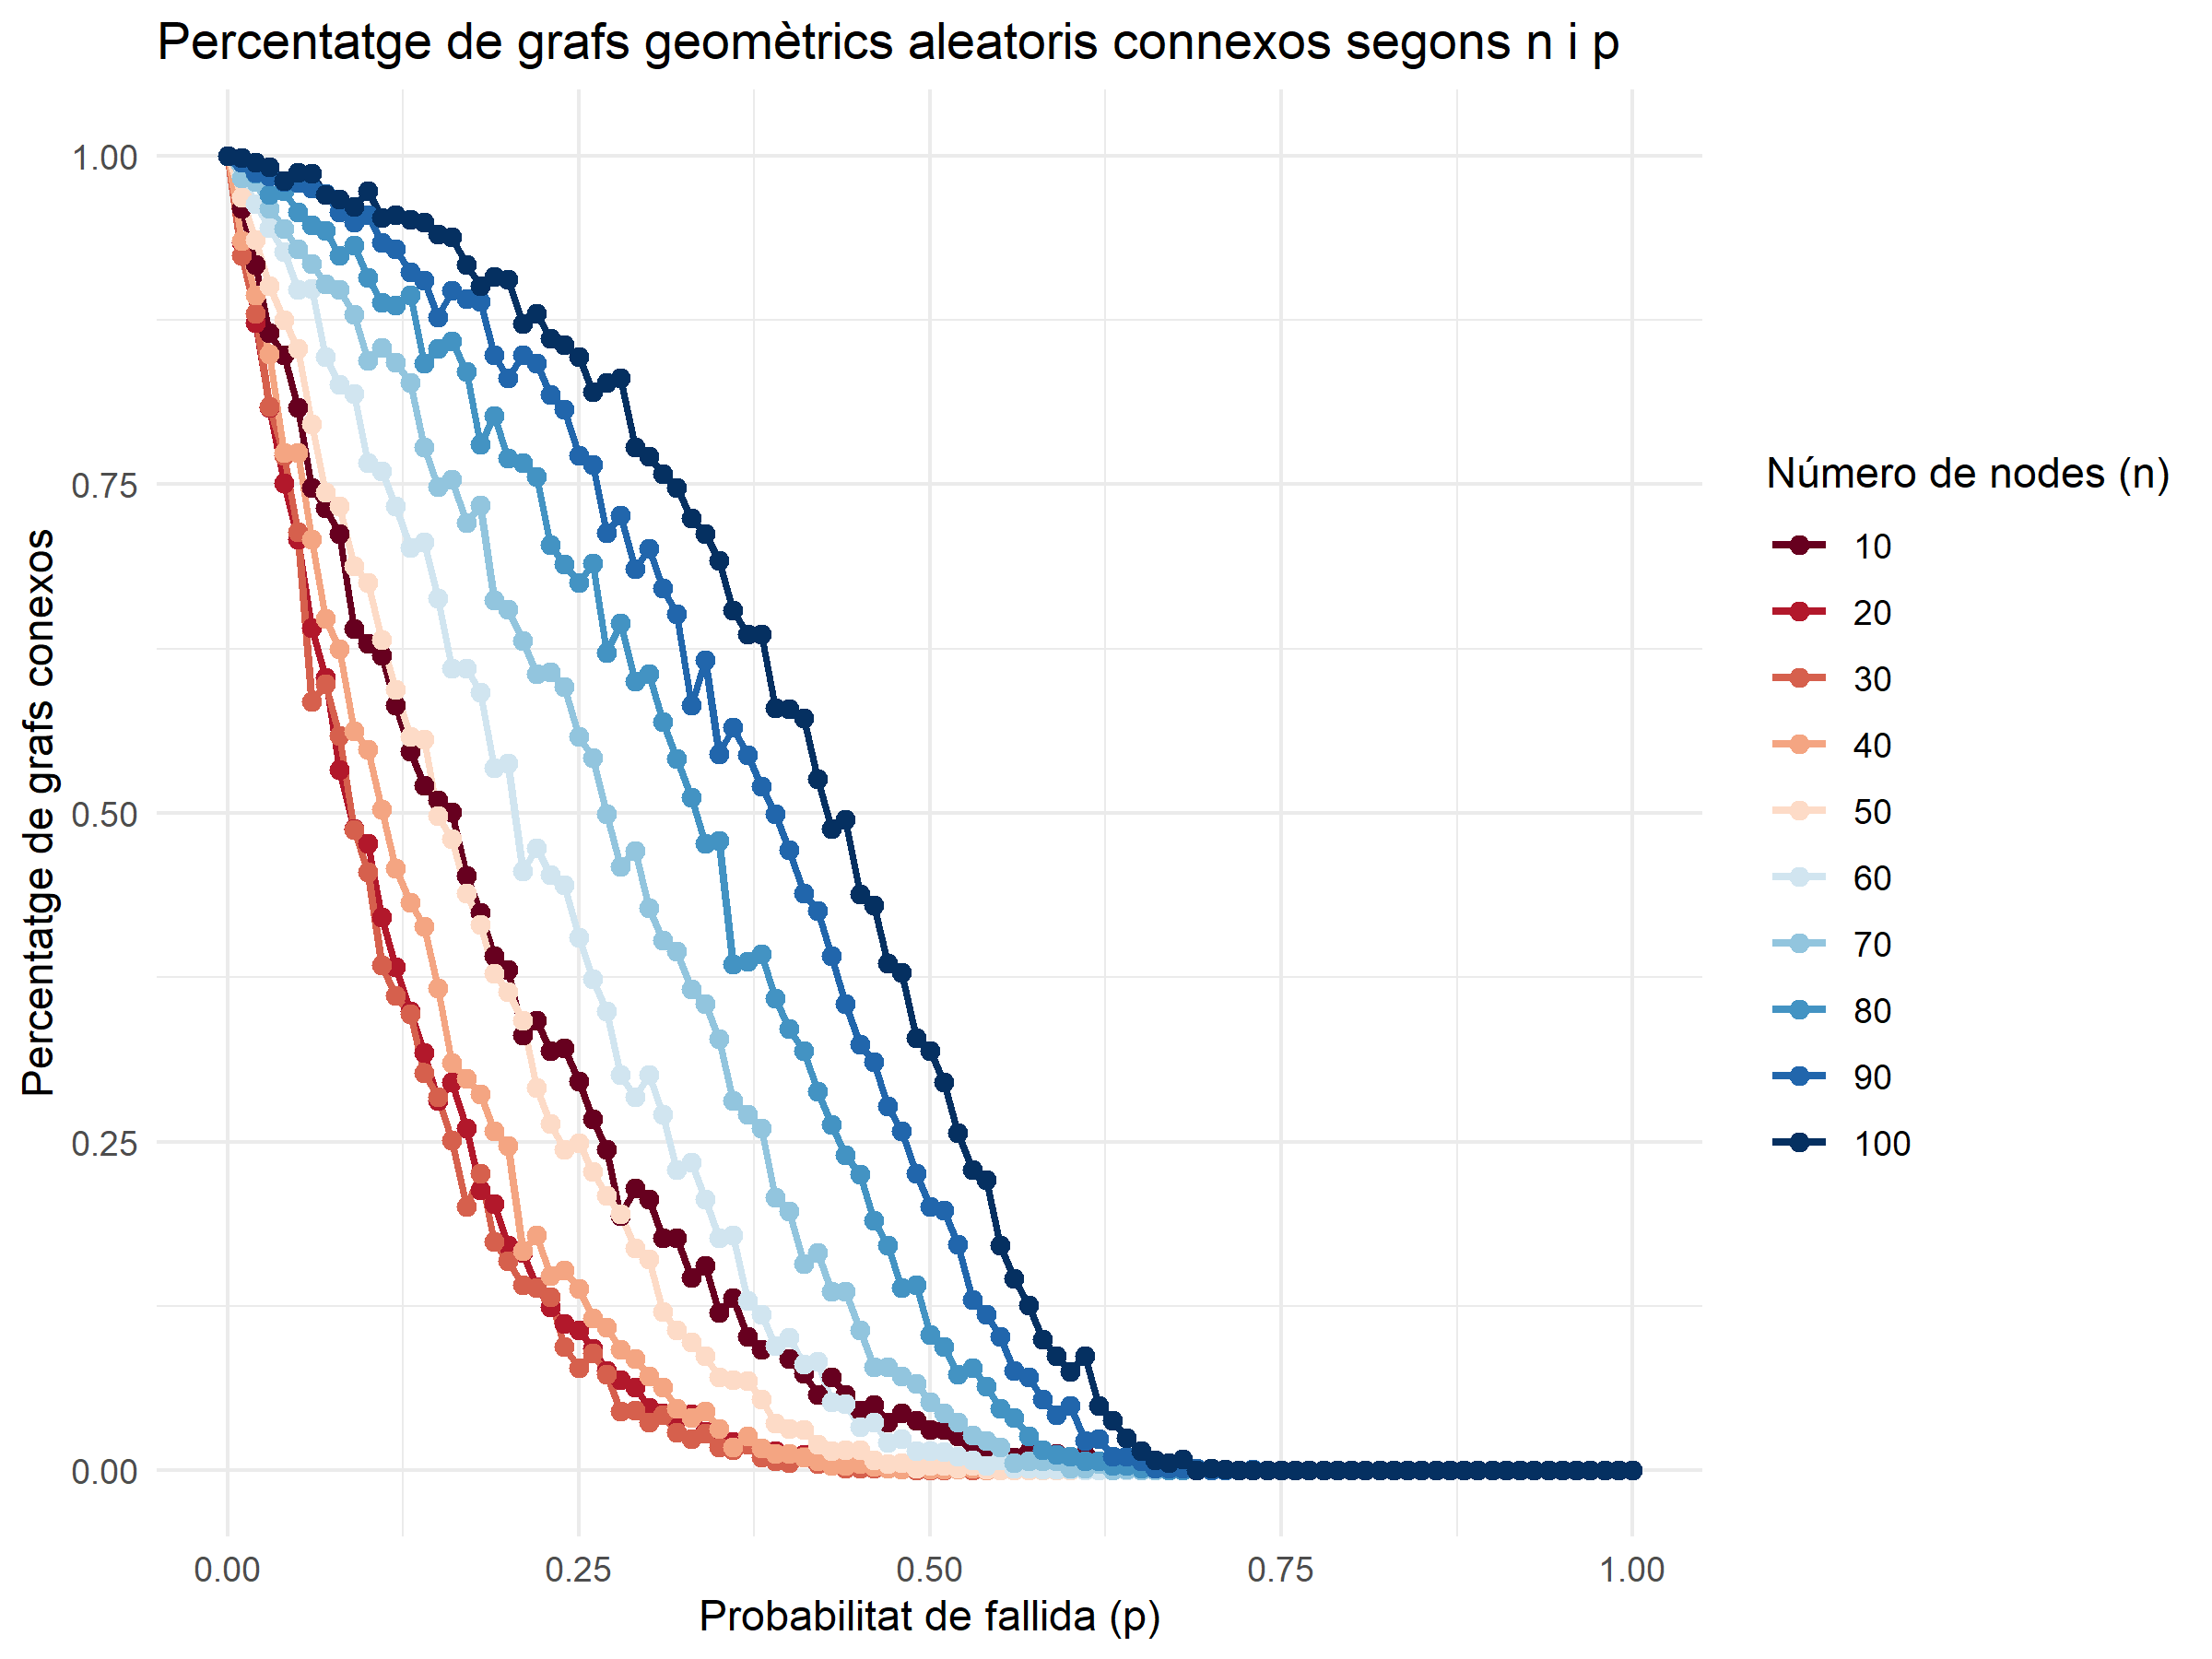
\includegraphics[width=\textwidth]{images/randomGeometric_10-100_0.2}
			\footnotesize{9283948 10 100 10 1000 EDGE\_PERC ./data/rgg10.csv Random-Geometric 0.2}
		\end{minipage}
		\hfill
		\begin{minipage}{0.45\textwidth}
			\centering
			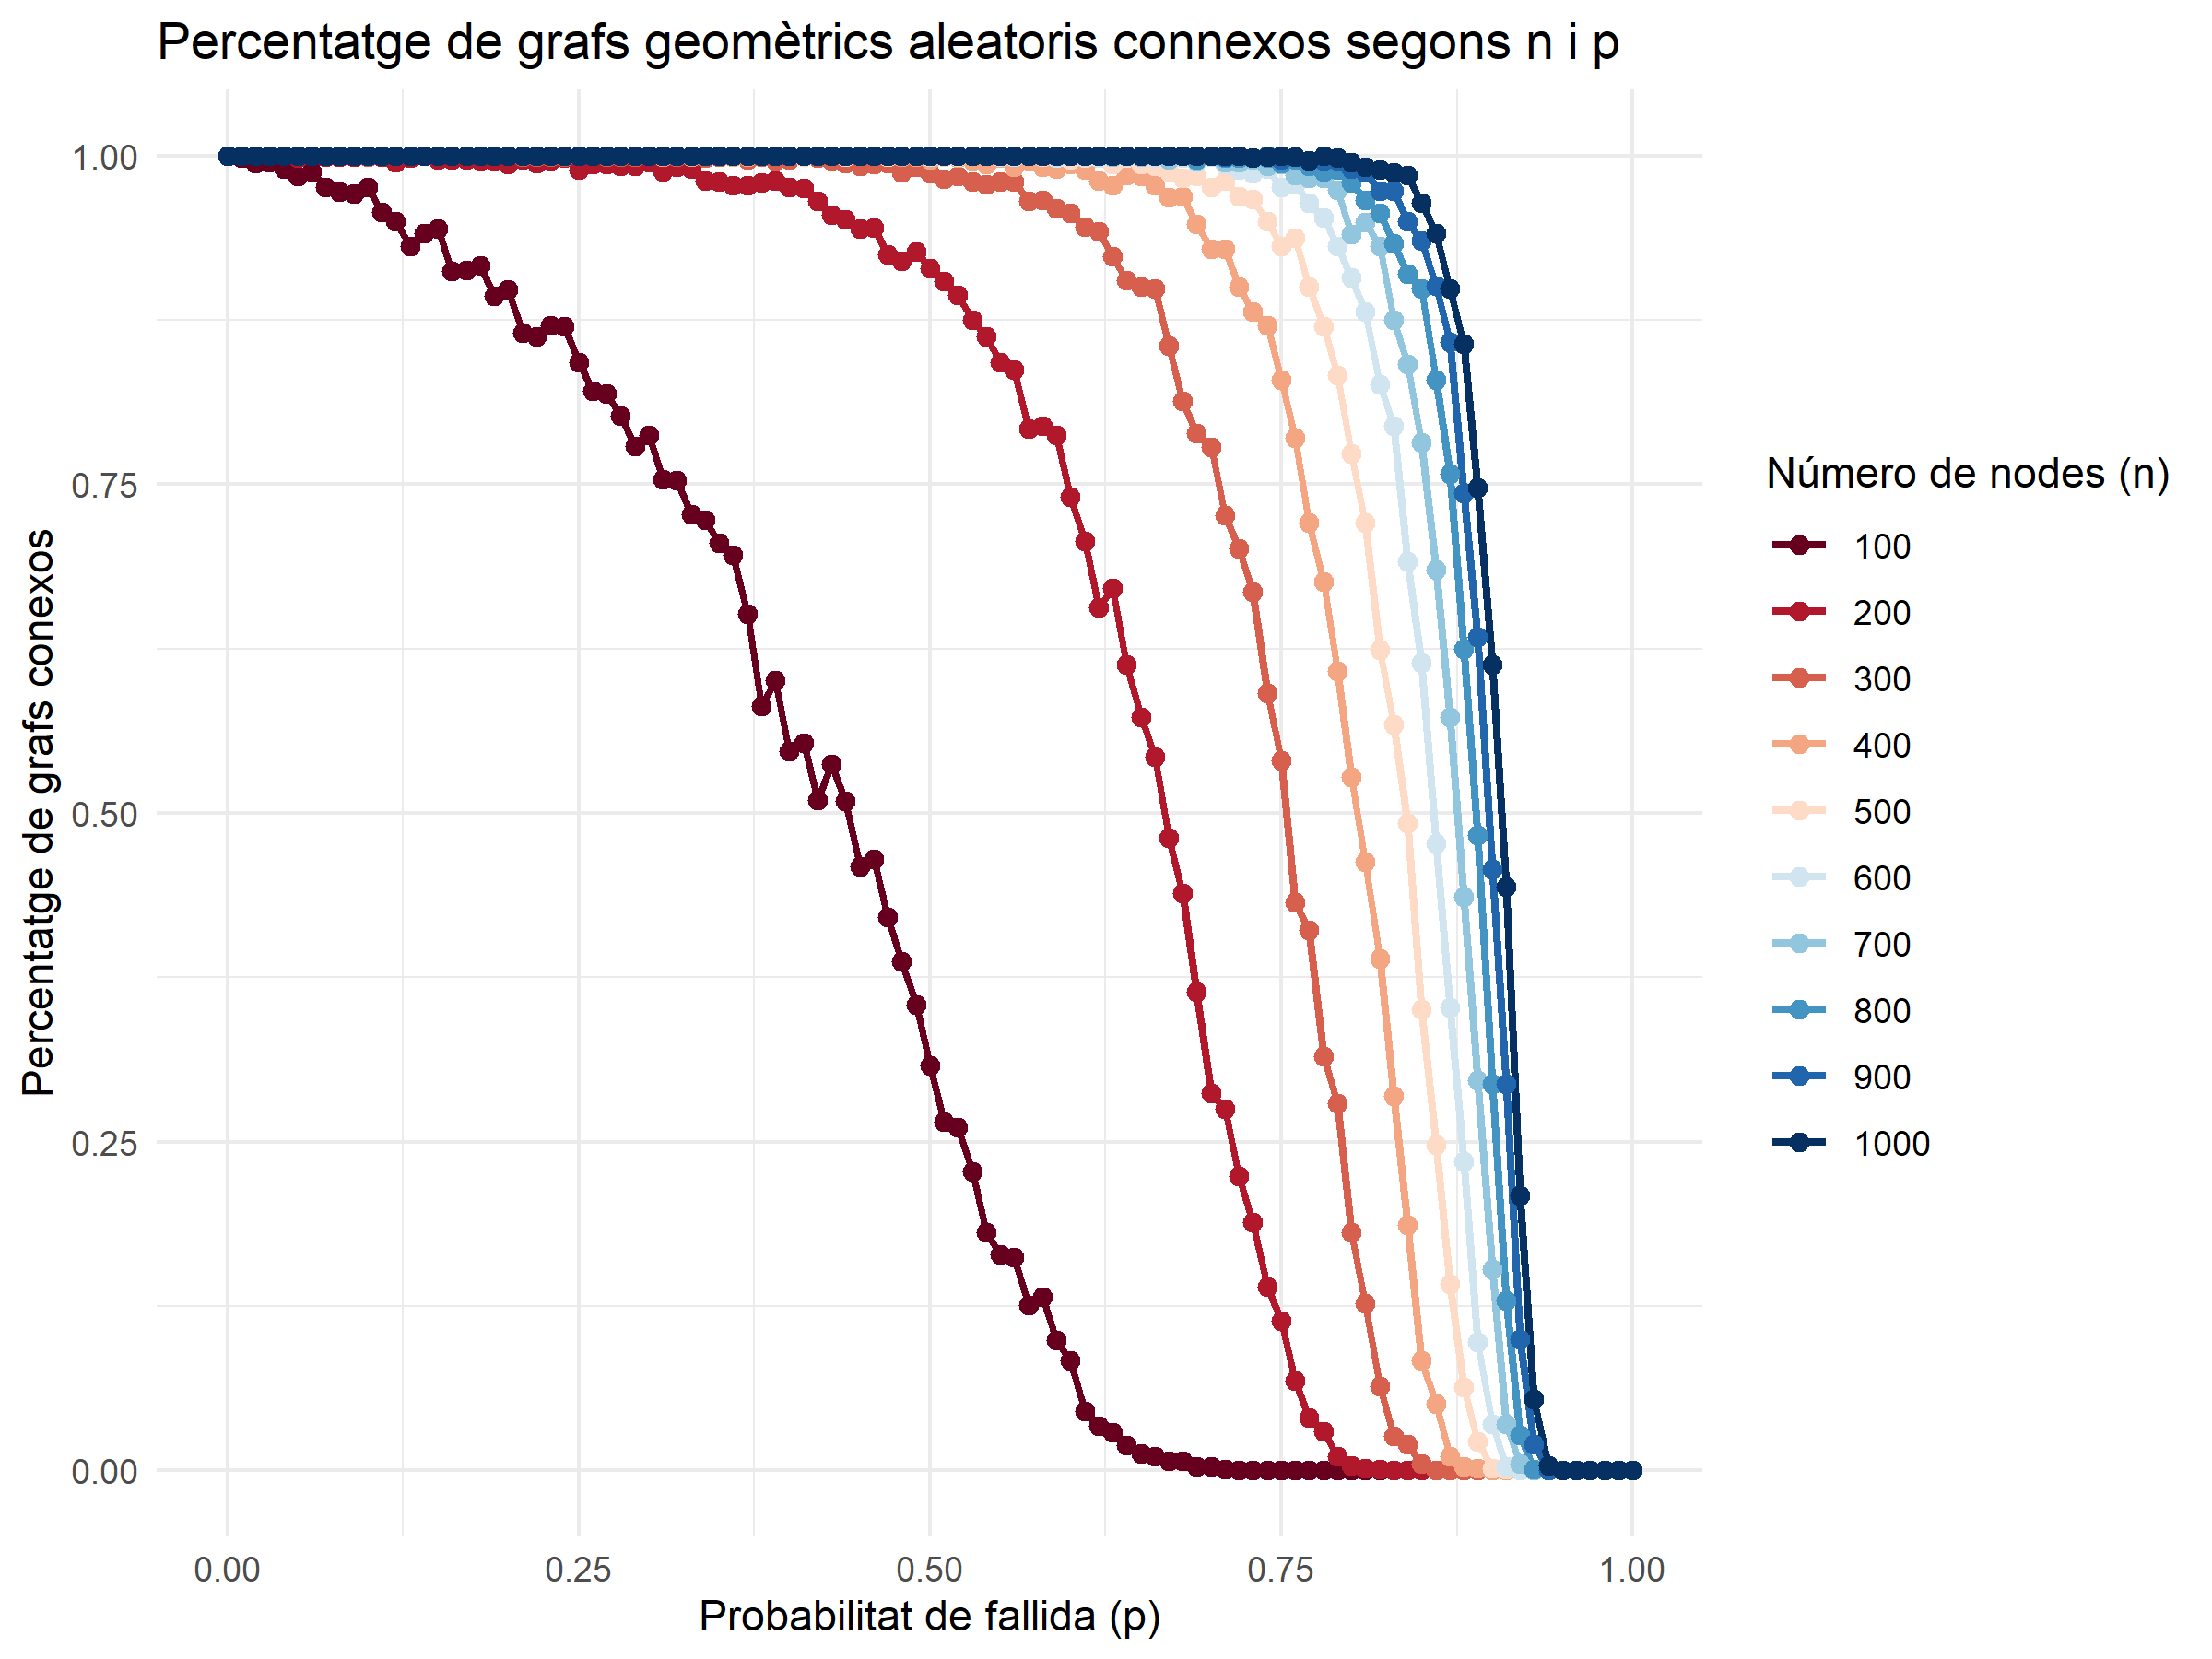
\includegraphics[width=\textwidth]{images/randomGeometric_100-1000_0.2}
			\footnotesize{9283948 10 100 10 1000 EDGE\_PERC ./data/rgg16.csv Random-Geometric 0.2}
		\end{minipage}
		\caption{Comparativa de percolació per arestes del grafs geometrics aleatoris amb $n$ = 10..100 (1) i $n$ = 100..1000 (2), $r$ = 0.2}
		\label{fig:percolation_edges_rgg_0.2}
	\end{figure}
	
	En aquesta primera comparativa, \textit{Figura \ref{fig:percolation_edges_rgg_0.2}}, veiem com grafs amb una connectivitat feble amb pocs nodes deixen de generar grafs connexos quan hi ha una probabilitat de percolació relativament baixa. No obstant, a mesura que augmenten els nodes, la quantitat de grafs connexos
	en funció de la probabilitat de percolació comença a creixer de manera notable (imatge 2). Això ens mostra que, tot i ser grafs amb una connectivitat teòrica feble, amb una quantitat de nodes suficientment gran es pot aconseguir una transició de fase tot i que la probabilitat
	de percolació sigui alta. 
	
	\begin{figure}[H]
		\centering
		\begin{minipage}{0.45\textwidth}
			\centering
			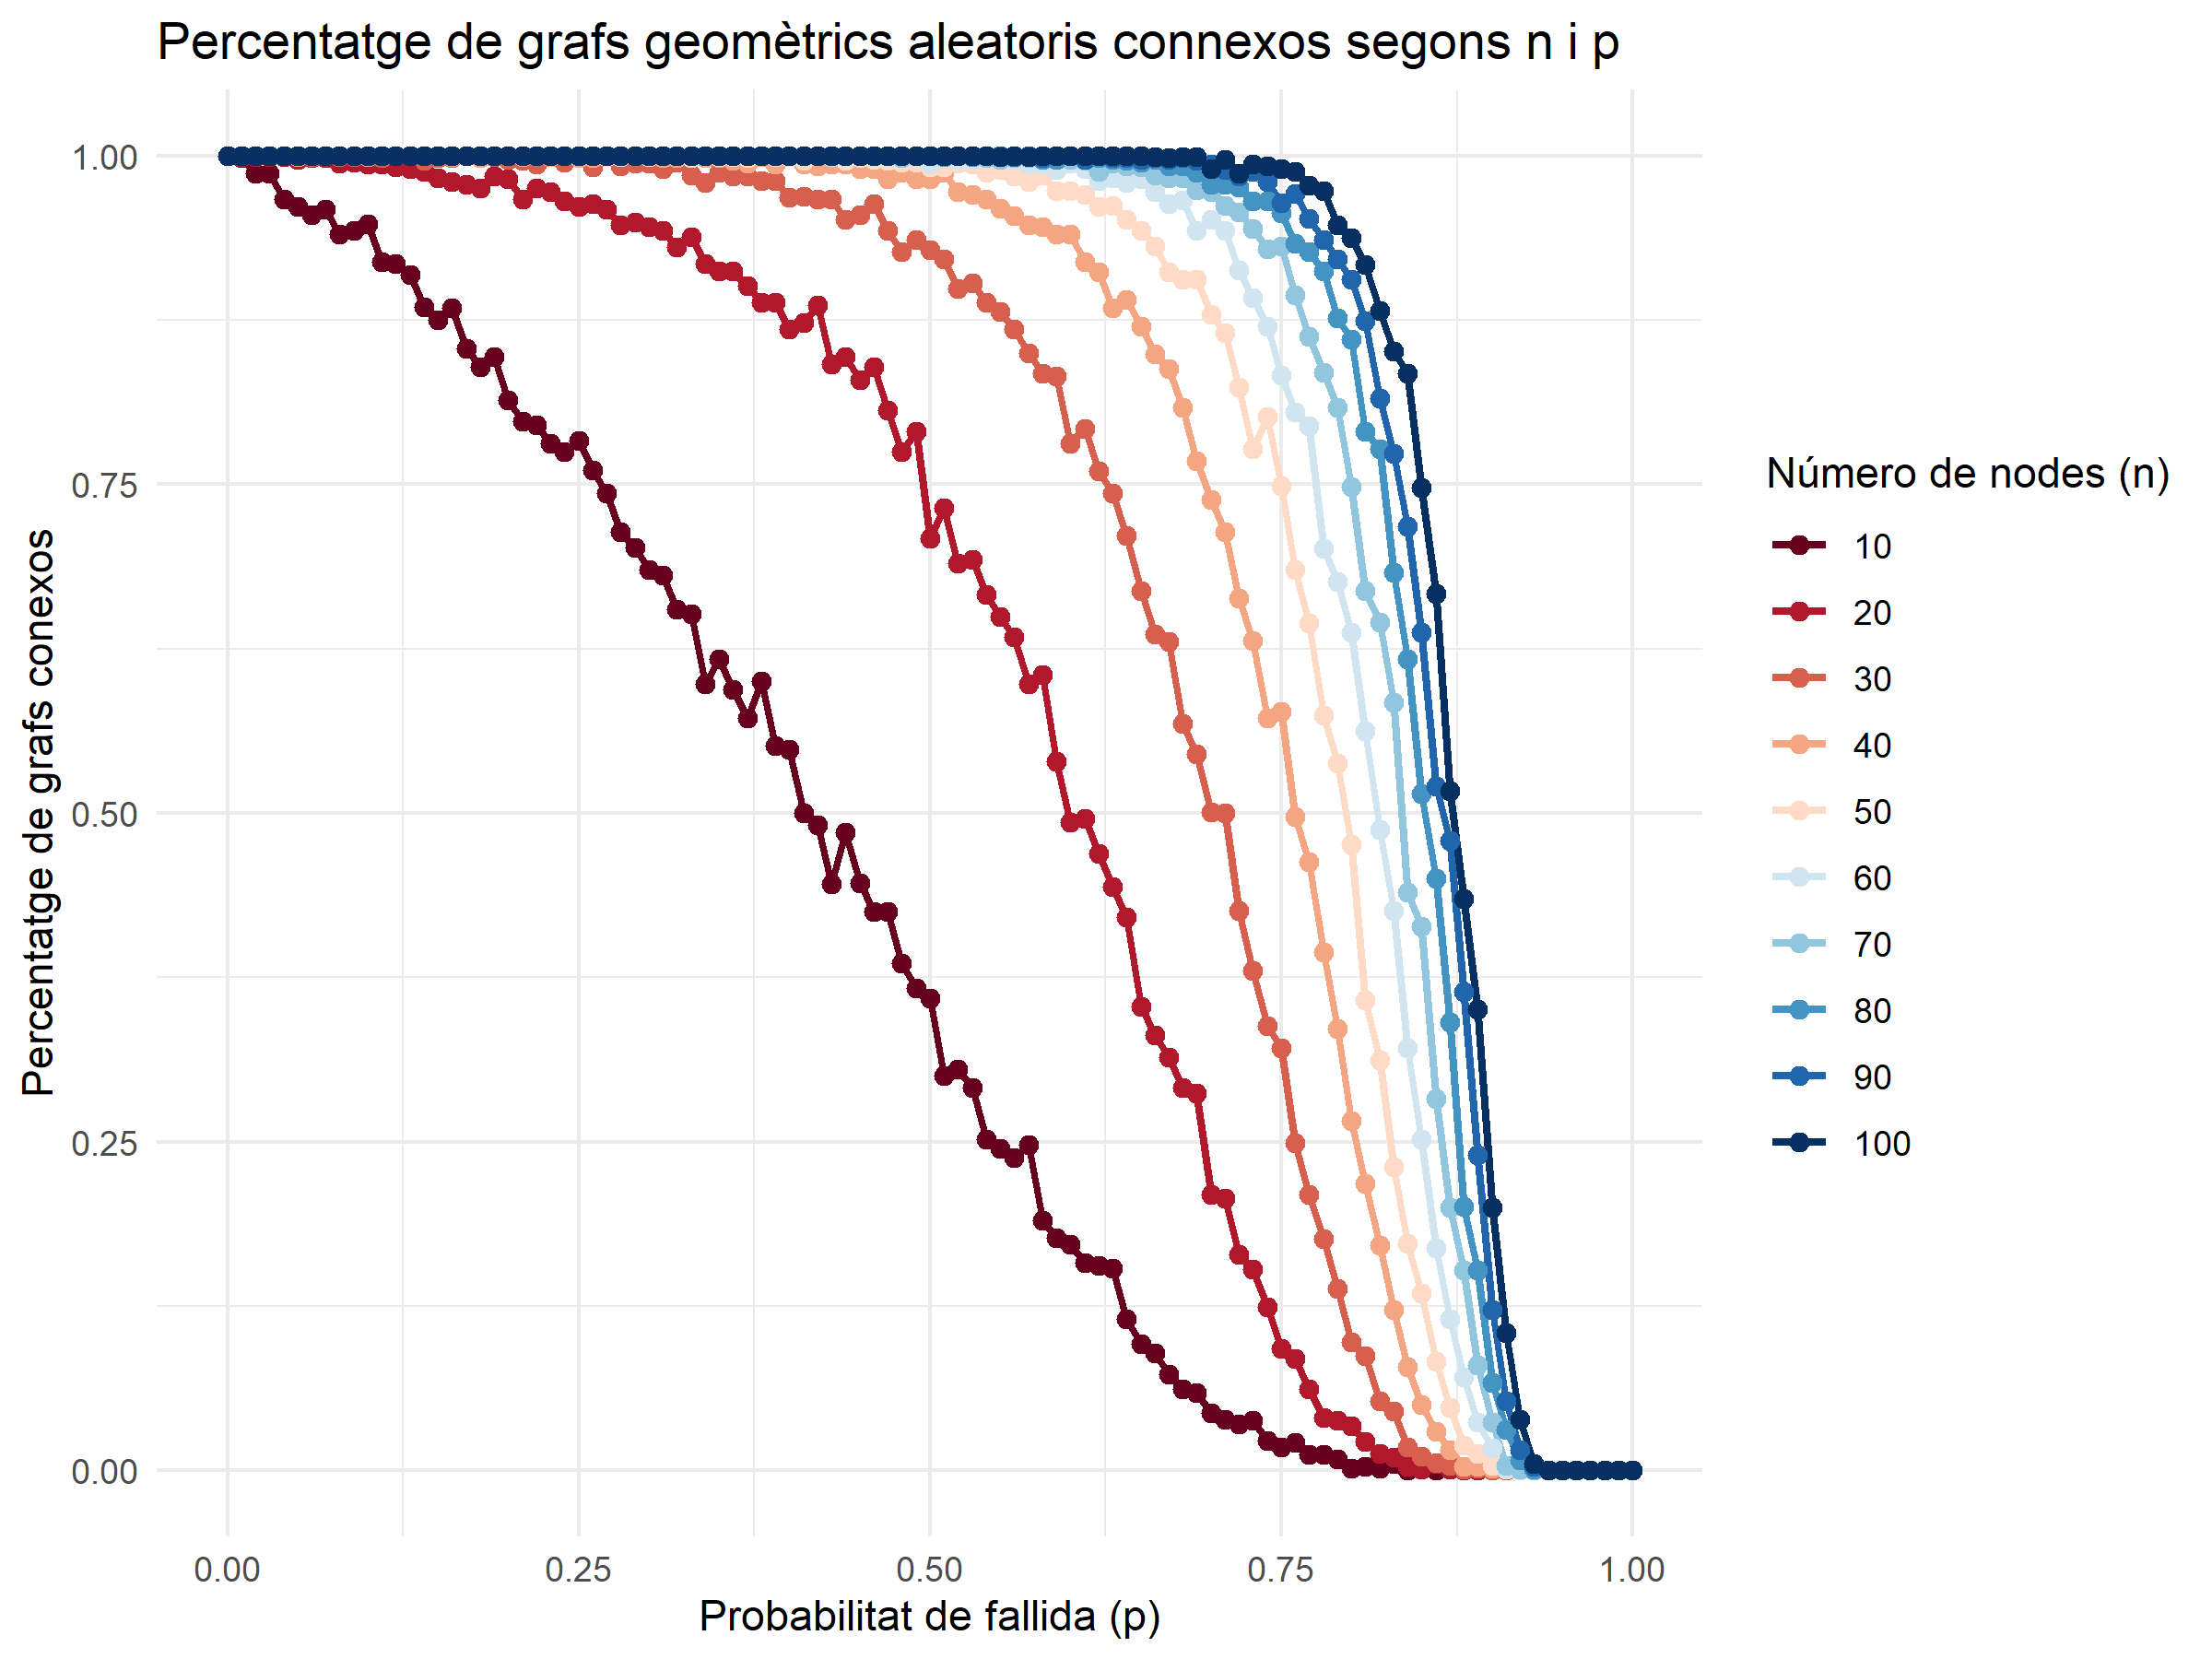
\includegraphics[width=\textwidth]{images/randomGeometric_10-100_0.5}
			\footnotesize{2389476 10 100 10 1000 EDGE\_PERC ./data/rgg11.csv Random-Geometric 0.5}
		\end{minipage}
		\hfill
		\begin{minipage}{0.45\textwidth}
			\centering
			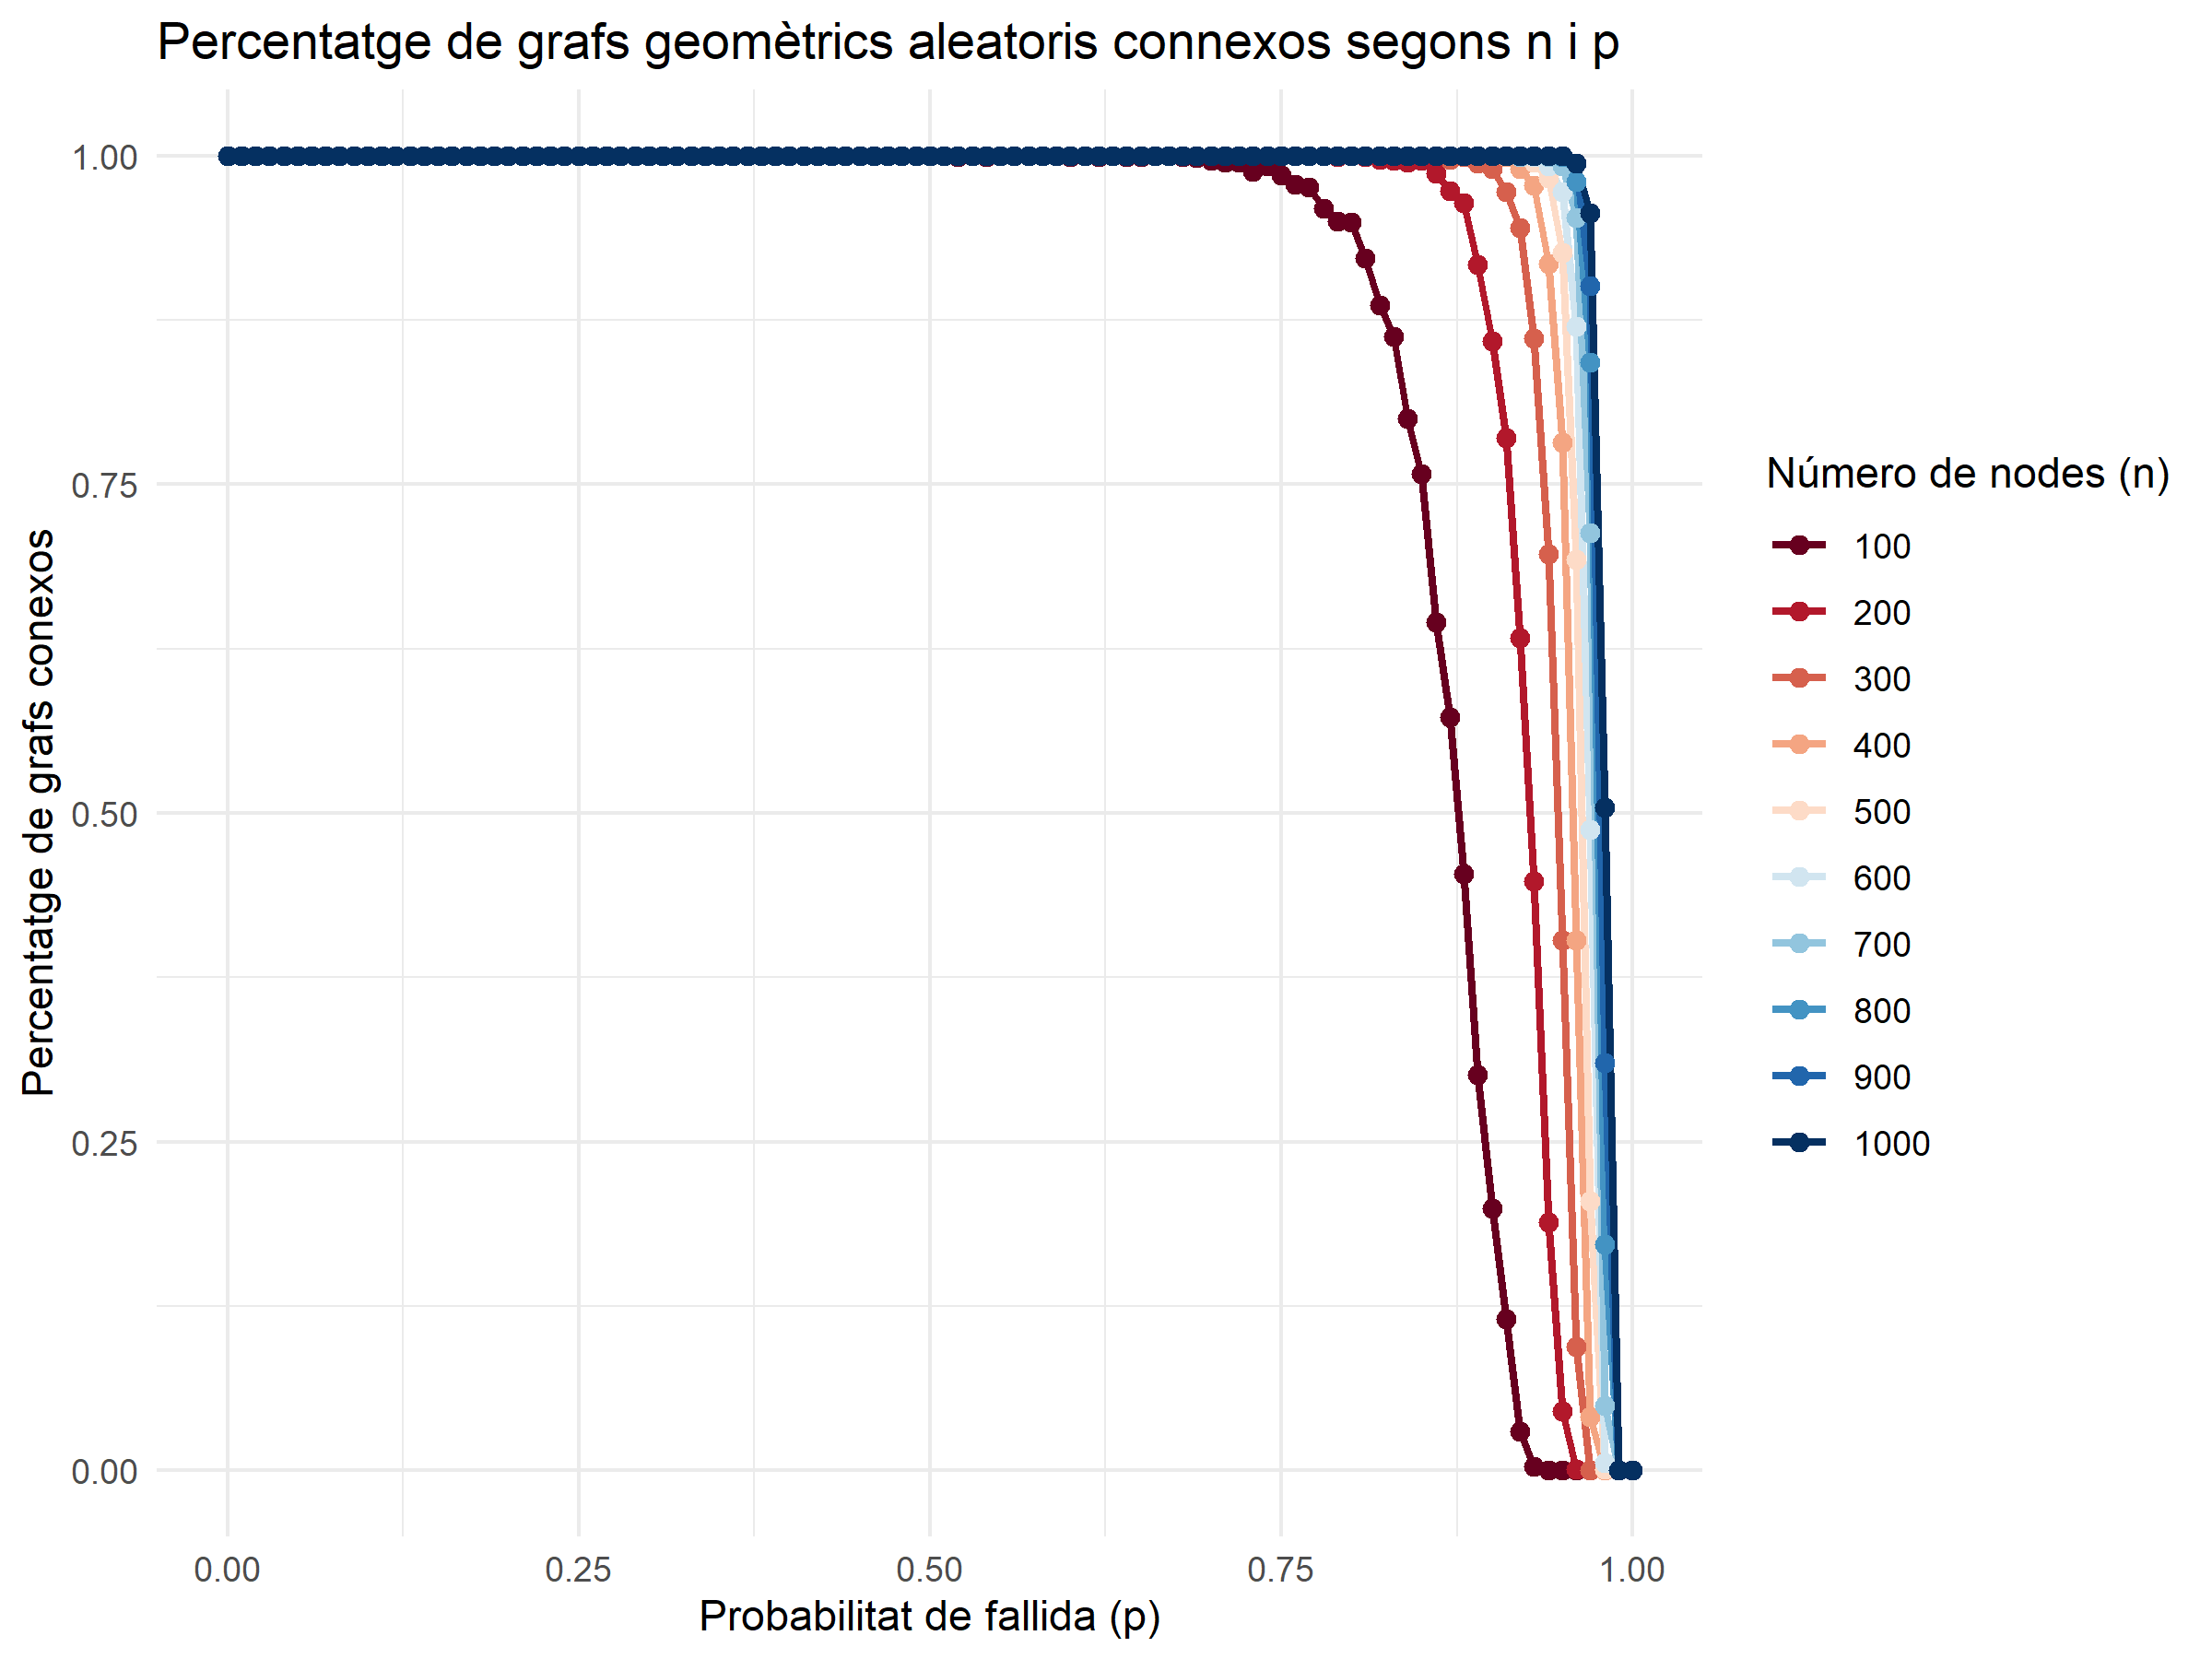
\includegraphics[width=\textwidth]{images/randomGeometric_100-1000_0.5}
			\footnotesize{6673428 100 1000 100 1000 EDGE\_PERC ./data/rgg17.csv Random-Geometric 0.5}
		\end{minipage}
		\caption{Comparativa de percolació per arestes del grafs geometrics aleatoris amb amb $n$ = 10..100 (1) i $n$ = 100..1000 (2), $r$ = 0.5}
		\label{fig:percolation_edges_rgg_0.5}
	\end{figure}
	
	Per altra banda, la \textit{Figura \ref{fig:percolation_edges_rgg_0.5}} mostra els resultats dels grafs amb una connectivitat teòrica major als anteriors. L'impacte d'aquesta connectivitat major es veu reflexat clarament en tots dos experients. En els casos de grafs amb una quantitat de nodes no gaire elevada, el percentatge de grafs connexos en funció de la probabilitat de percolació és bastant elevat fins i tot per al cas de grafs d'únicament 10 nodes (imatge esquerra). Més enllà d'aquesta quantitat, el percentatge incrementa de forma notòria fins a arribar un punt en el que la diferència entre les probabilitats de percolació per a cada quantitat de nodes és irrisoria.
	
	
	\begin{figure}[H]
		\centering
		\begin{minipage}{0.45\textwidth}
			\centering
			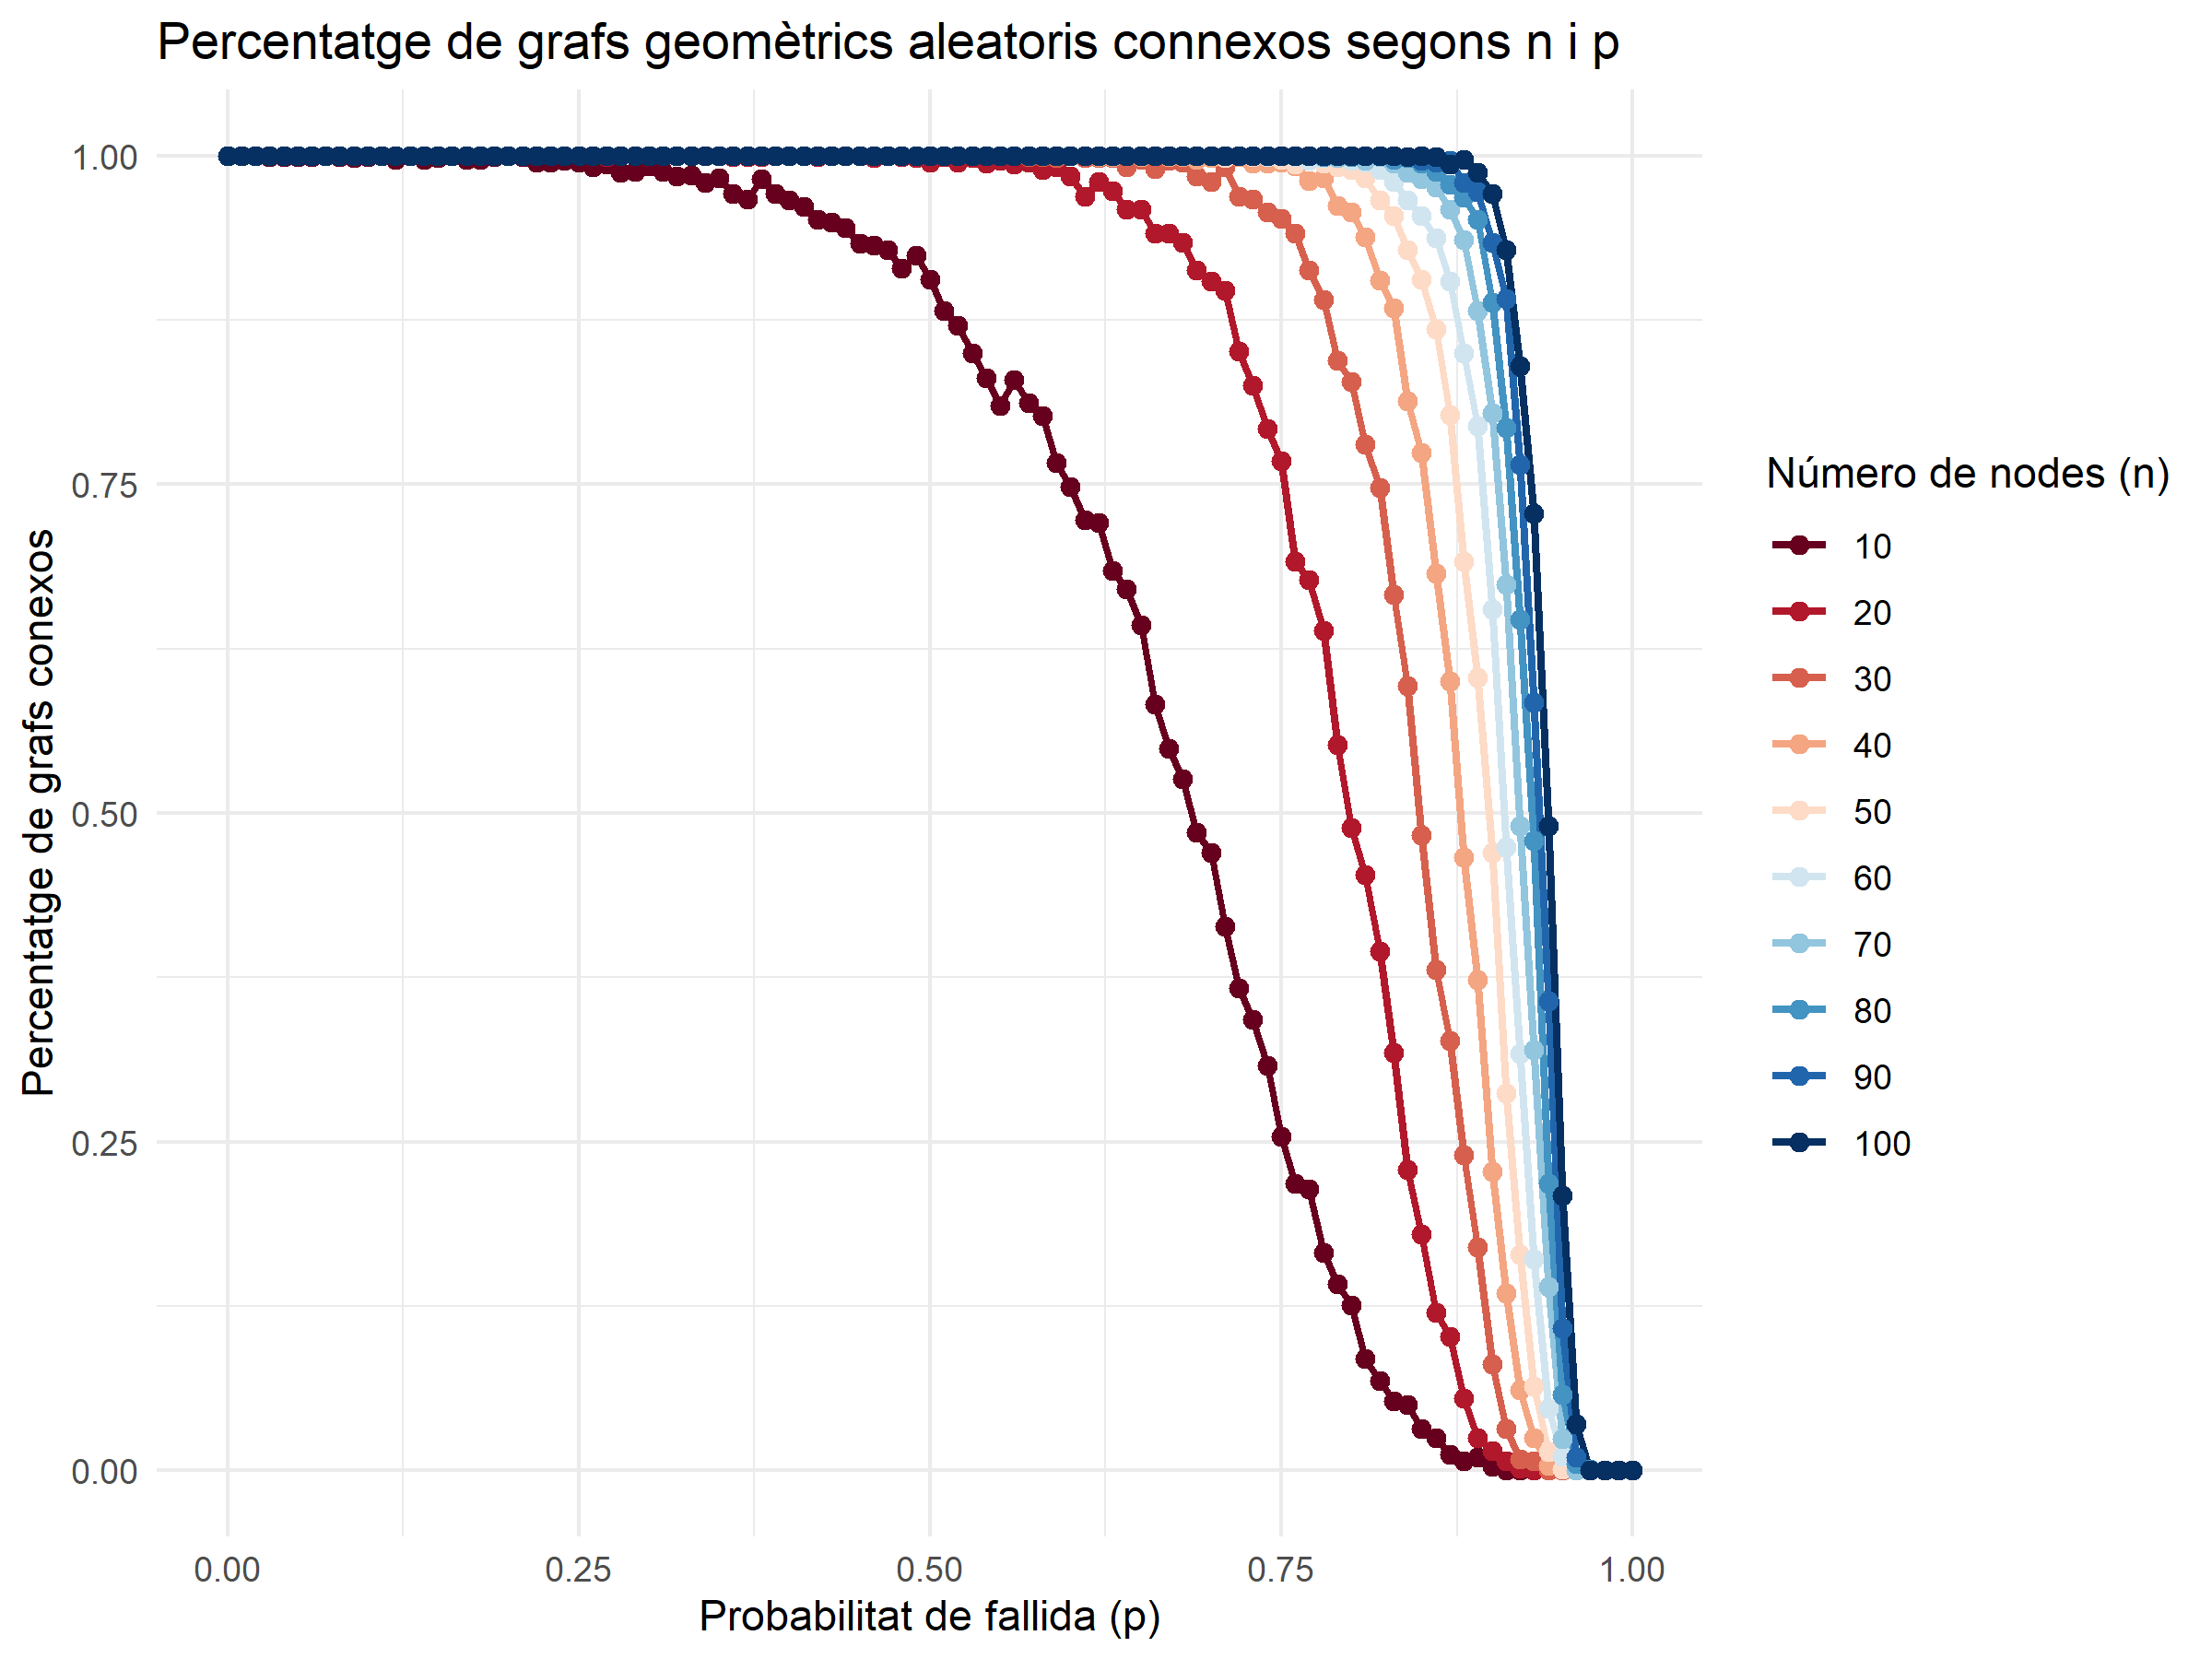
\includegraphics[width=\textwidth]{images/randomGeometric_10-100_0.8}
			\footnotesize{8273563 10 100 10 1000 EDGE\_PERC ./data/rgg12.csv Random-Geometric 0.8}
		\end{minipage}
		\hfill
		\begin{minipage}{0.45\textwidth}
			\centering
			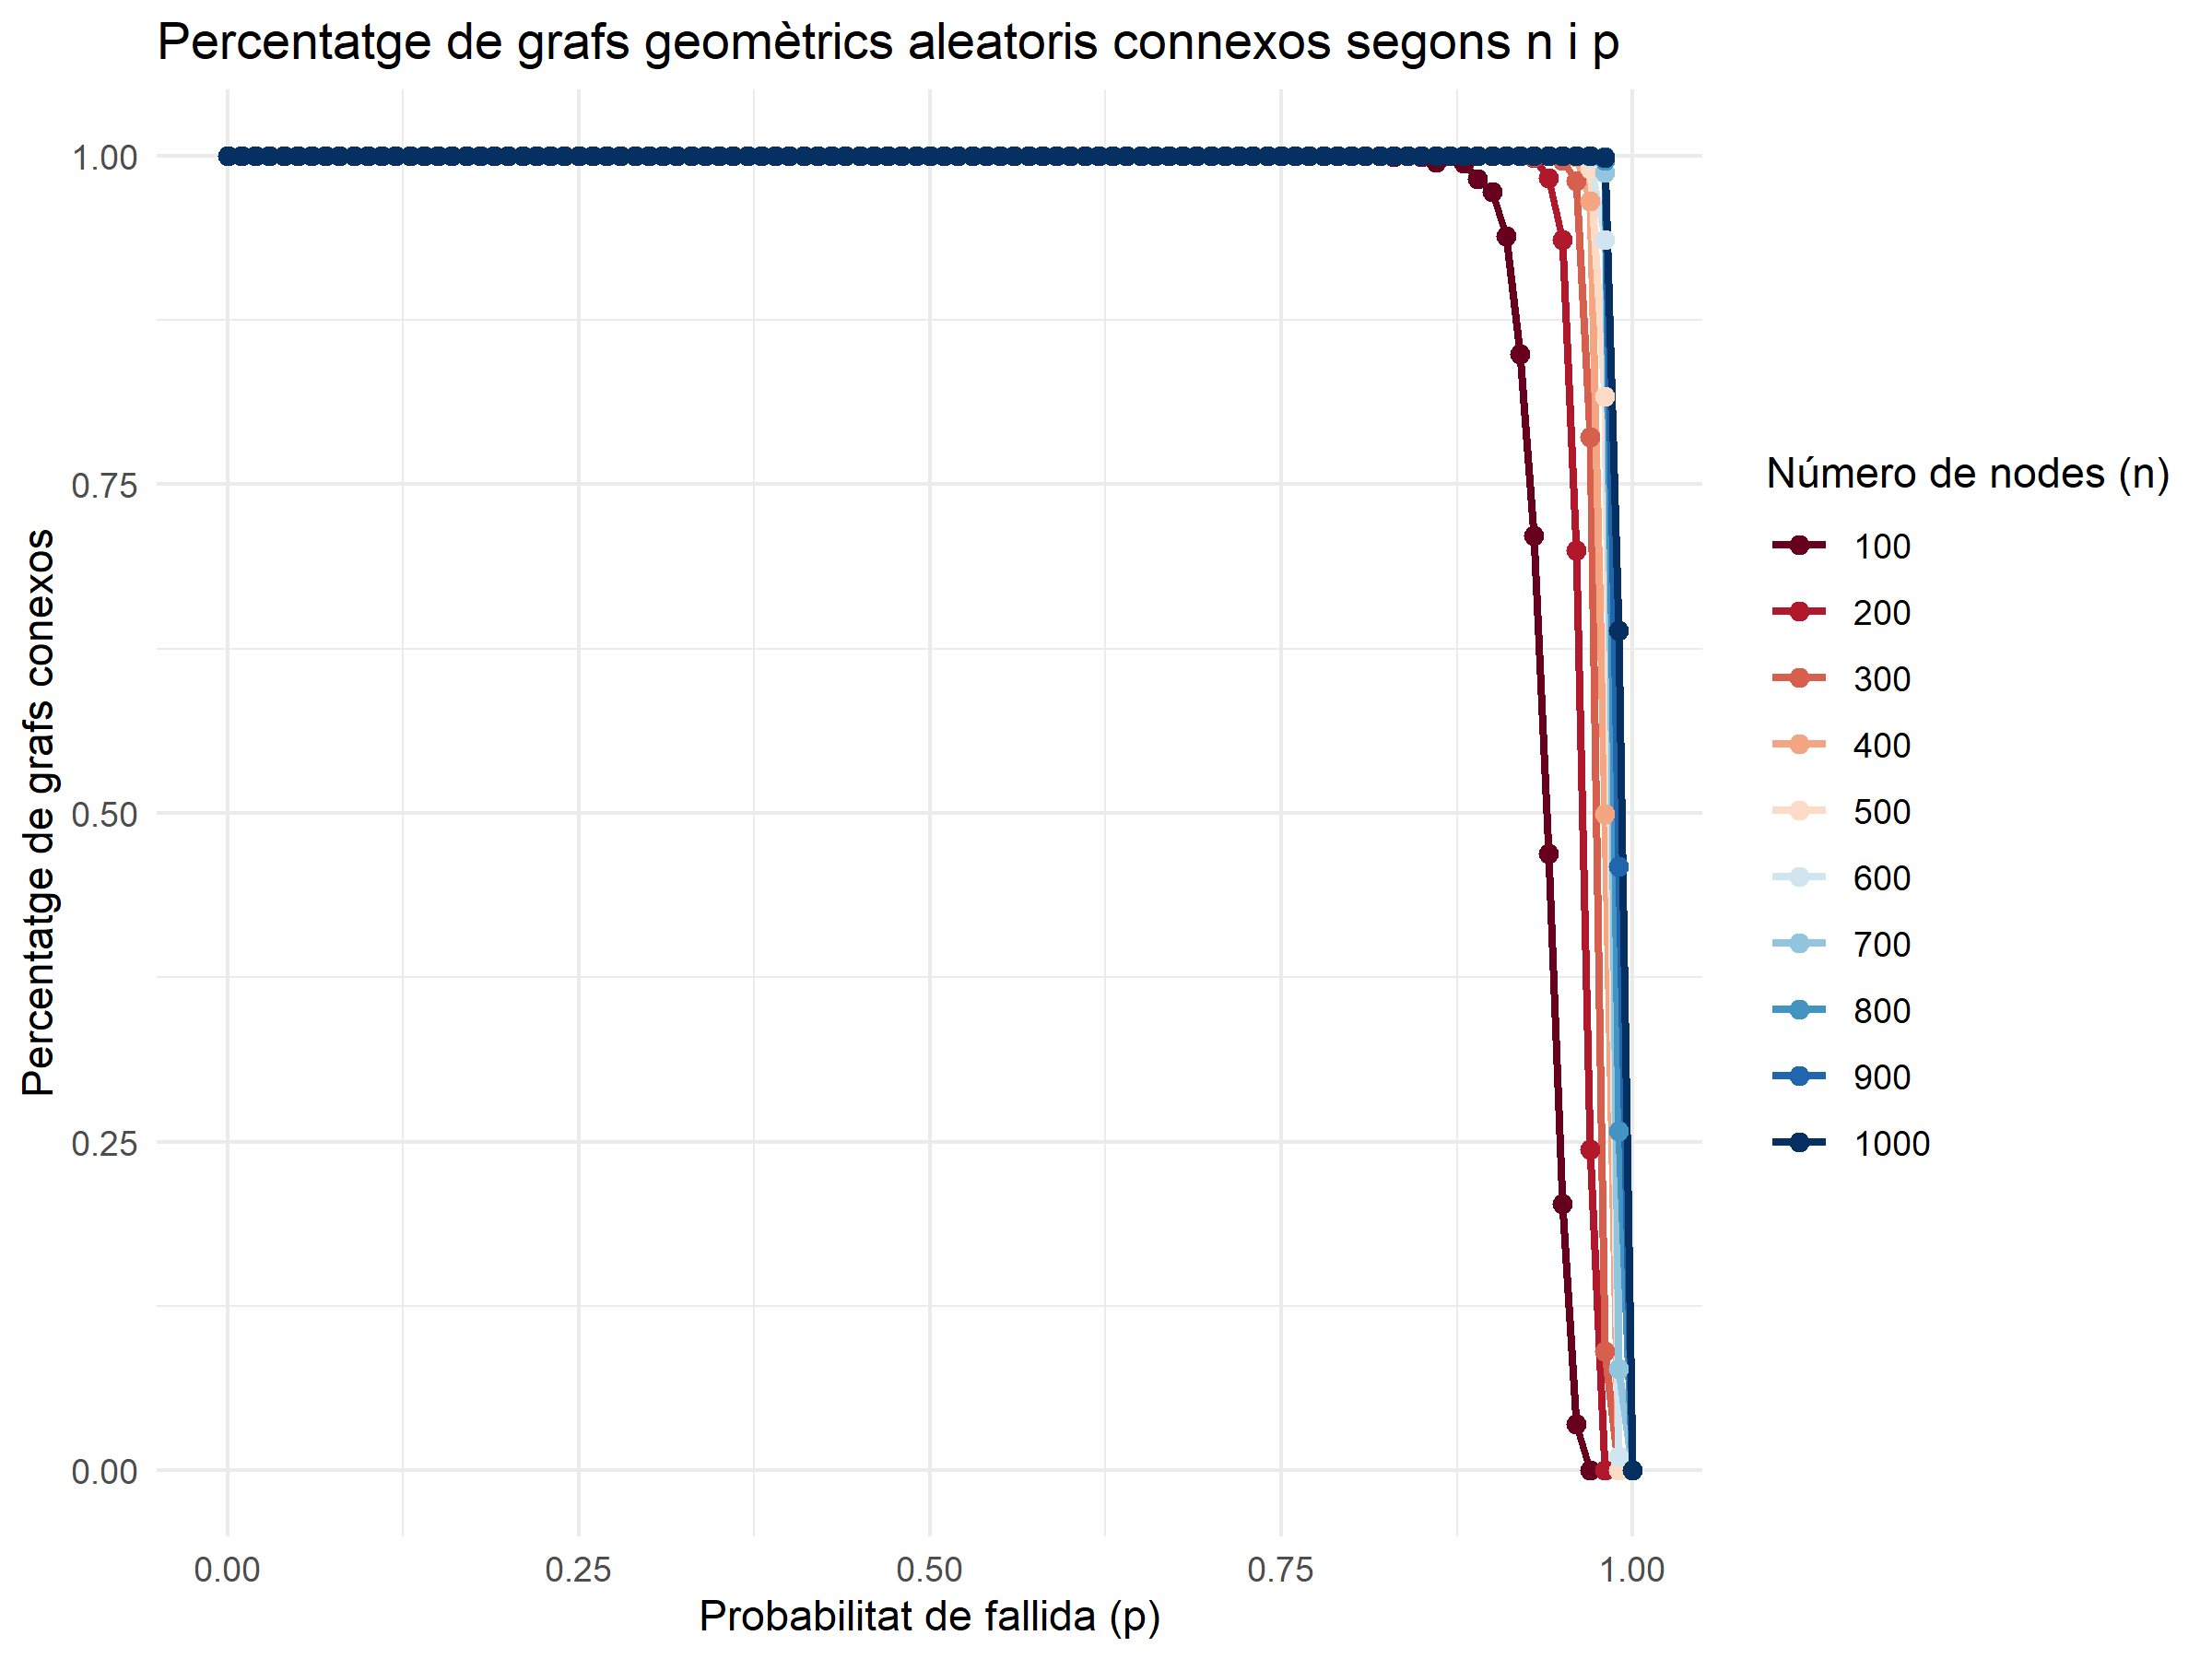
\includegraphics[width=\textwidth]{images/randomGeometric_100-1000_0.8}
			\footnotesize{9293745 100 1000 100 1000 EDGE\_PERC ./data/rgg18.csv Random-Geometric 0.8}
		\end{minipage}
		\caption{Comparativa de percolació per arestes del grafs geometrics aleatoris amb $n$ = 10..100 (1) i $n$ = 100..1000 (2), $r$ = 0.8}
		\label{fig:percolation_edges_rgg_0.8}
	\end{figure}
	
	Per últim, a \textit{Figura \ref{fig:percolation_edges_rgg_0.8}} s'utilitzen grafs geometrics aleatoris amb un radi de connectivitat molt elevat, donant-lis una forma seblant a un graf complet. Per aquest motiu, fins que la probabilitat de percolació no és molt alta, els grafs generats segueixen
	sent connexos una vegada aplicada la transició de fase. Evidentment, l'augment de nodes provoca que el percentatge de grafs connexos creixi ja que els nodes tenen més probabilitats d'estar units a altres nodes (imatge 2), fet que ha succeït a totes les comparatives.
	
	\subsection{Graf de Barabási-Albert}
	
	L'estudia que s'ha realitzat sobre els grafs generats amb el model de Barabási-Albert és un de transició de fase sota percolació per nodes. El motiu és que es vol veure l'impacte d'una percolació a un graf que conté molts vertexs units entre sí per un o més "hubs" centrals, l'impacte que tindria la fallida d'algun d'aquests nodes o, per altra banda, el no impacte que pot tenir sobre nodes que tenen una estructura de fulla, és a dir, nodes que estan connectats unicament a un altre node i pertant la seva fallida segueix permetent un graf connex. \\
	
	Els experiments realitzats sobre aquests grafs depenen de tres paràmetres: nombre de nodes $n$, nombre de nodes inicials o \textit{hubs} $m0$, i el nombre d'arestes que han de tenir com a mínim cada node que no és \textit{hub}. Per als nostres experiments, hem decidit donar els següents valors: per al nombre de nodes $n = 10..100$, $n = 50..500$, per al nombre inicial de nodes o "hubs" $m0 = 2$, $m0 = 5$, $m0 = 10$, i per el nombre d'arestes incidents a la resta de nodes $m = 1$, $m = 2$, $m = 5$. Abans de veure els resultats, hem cregut adient une explicació del perqué s'han agafat aquests valors i no d'altres. Els grafs construïts amb el model de Barabási-Albert són típicament utilitzats com a xarxes on els nodes s'uneixen mitjançant "hubs". Per aquest motiu, hem decidit utilitzar aquests valors ja que representen d'una manera bastant realista una xarxa generada per aquest model d'una manera computacionalment viable. \\
	
	\subsubsection{Percolació per nodes}
	
	\begin{figure}[H]
		\centering
		\begin{minipage}{0.45\textwidth}
			\centering
			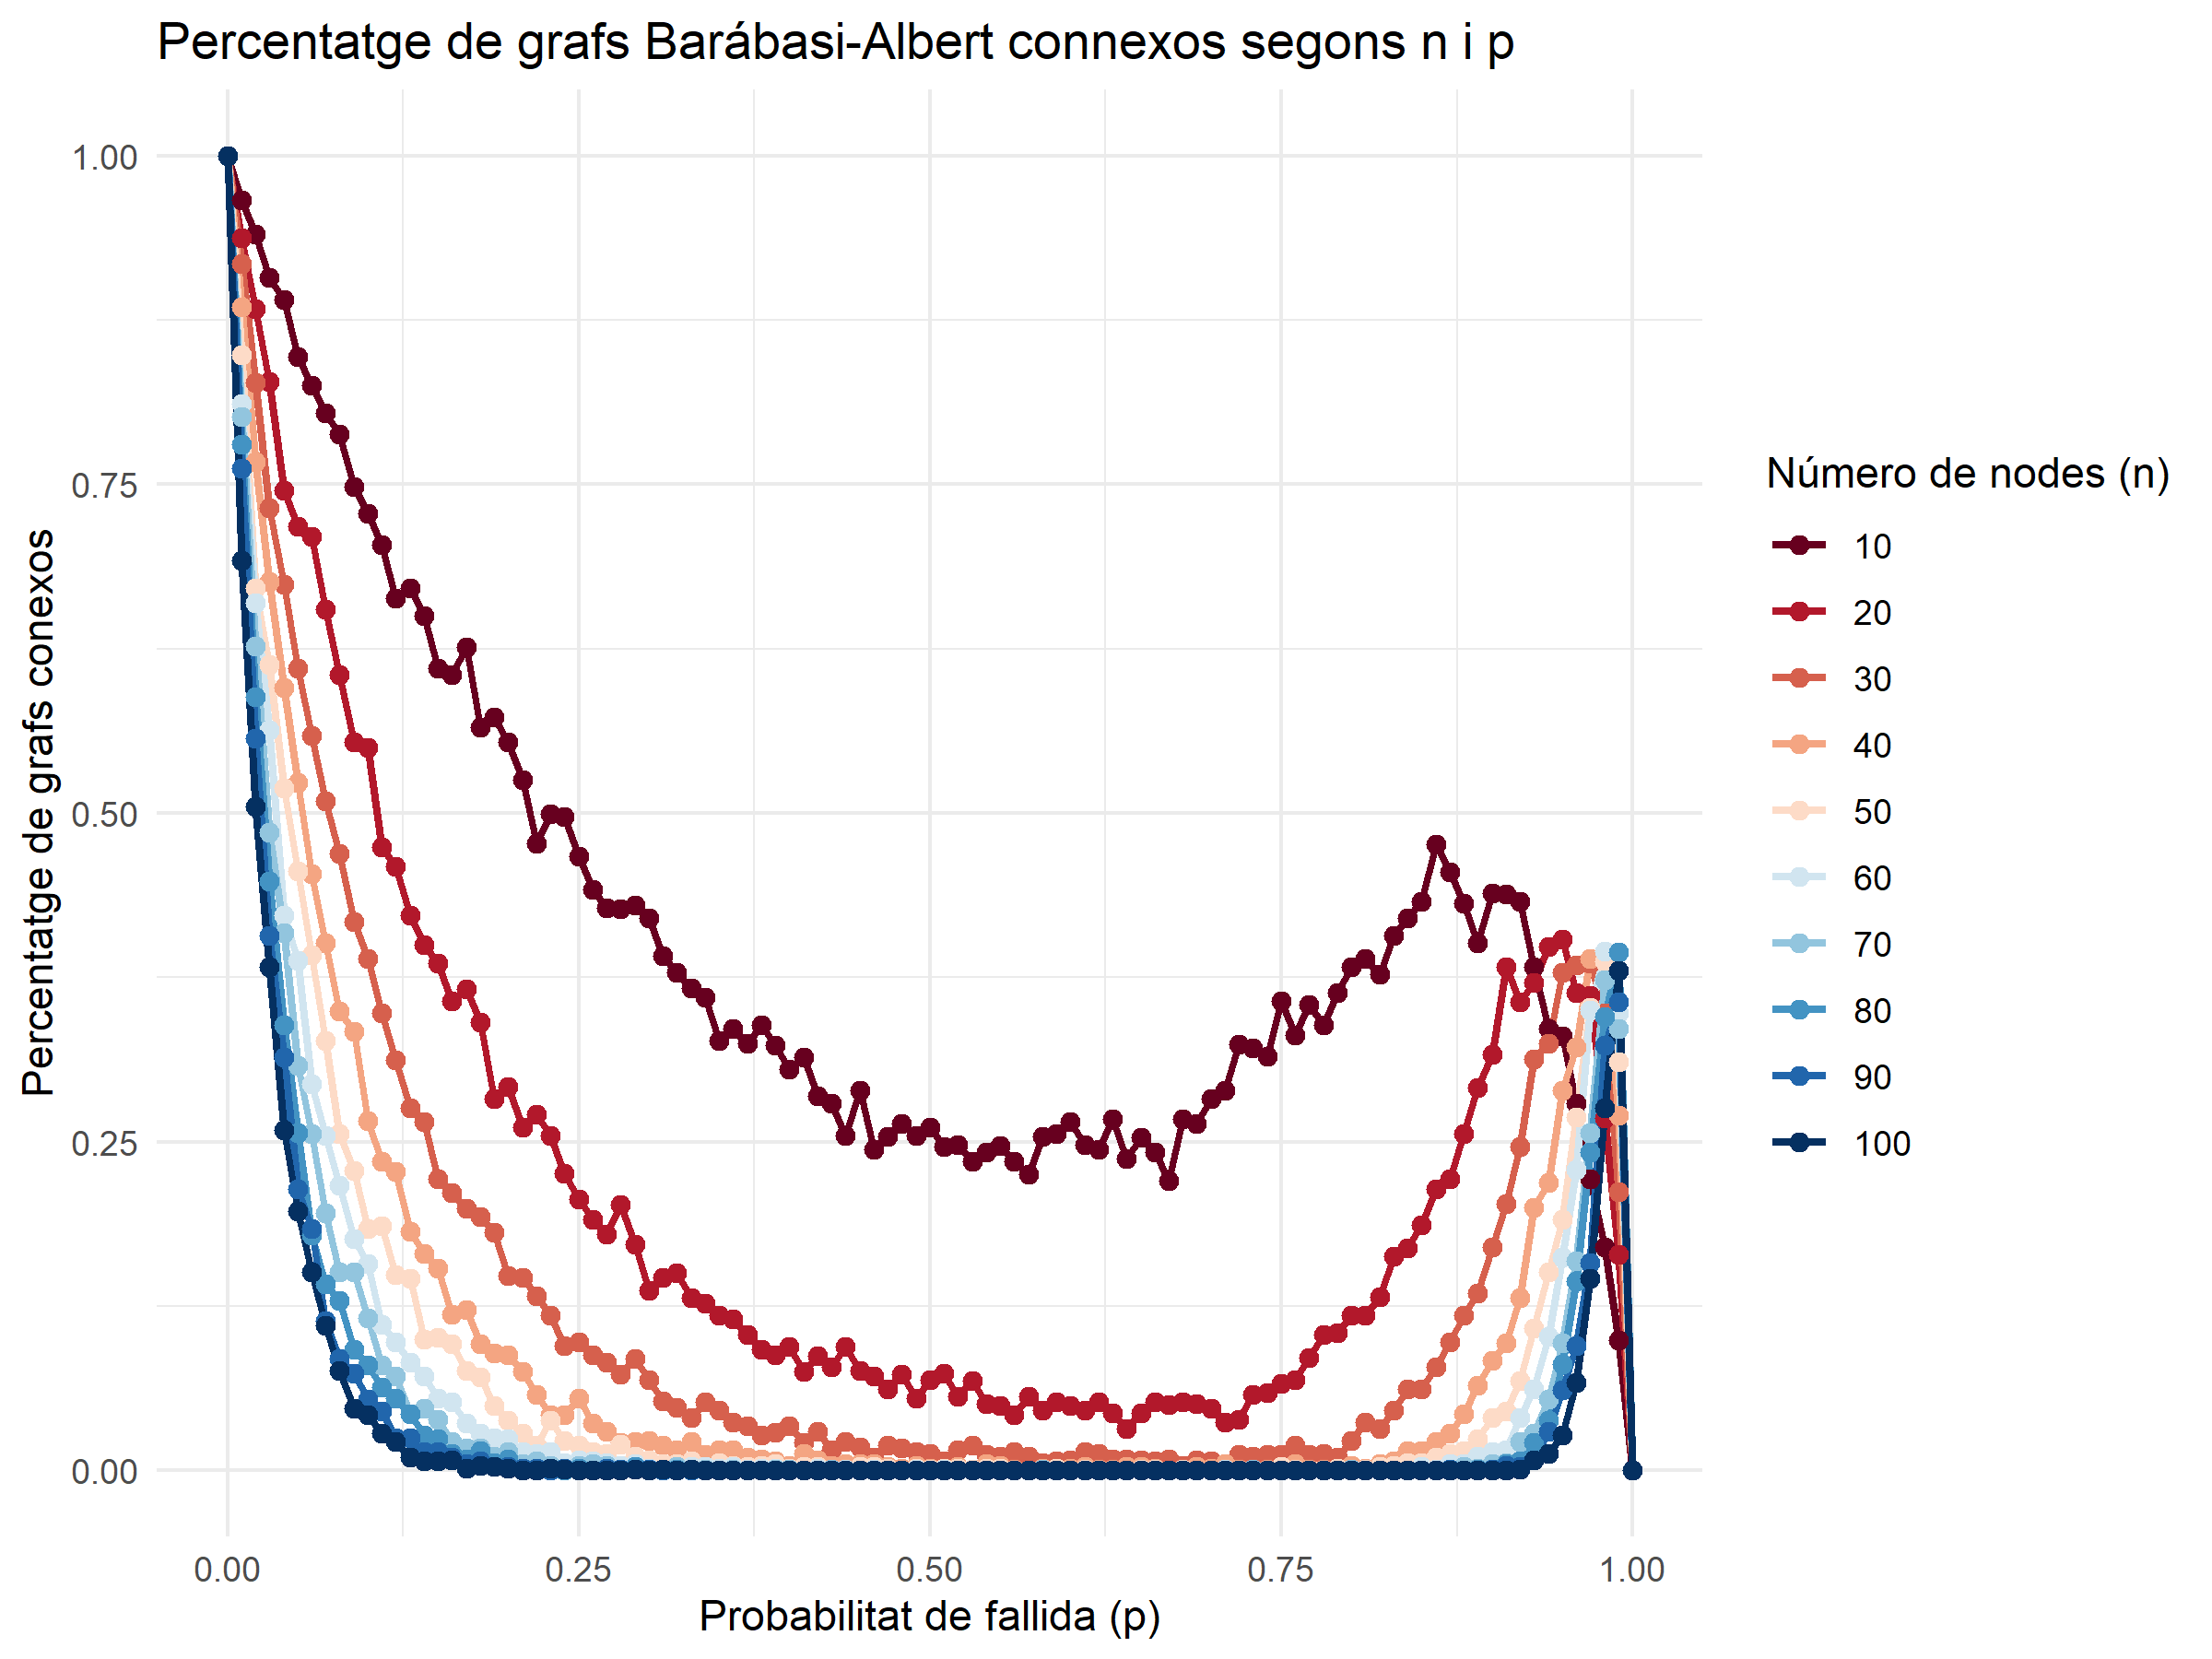
\includegraphics[width=\textwidth]{images/barabasi_10-100_2_1}
			\footnotesize{4575745 10 100 10 1000 NODE\_PERC ./data/ba9.csv Barabasi-Albert 2 1}
		\end{minipage}
		\hfill
		\begin{minipage}{0.45\textwidth}
			\centering
			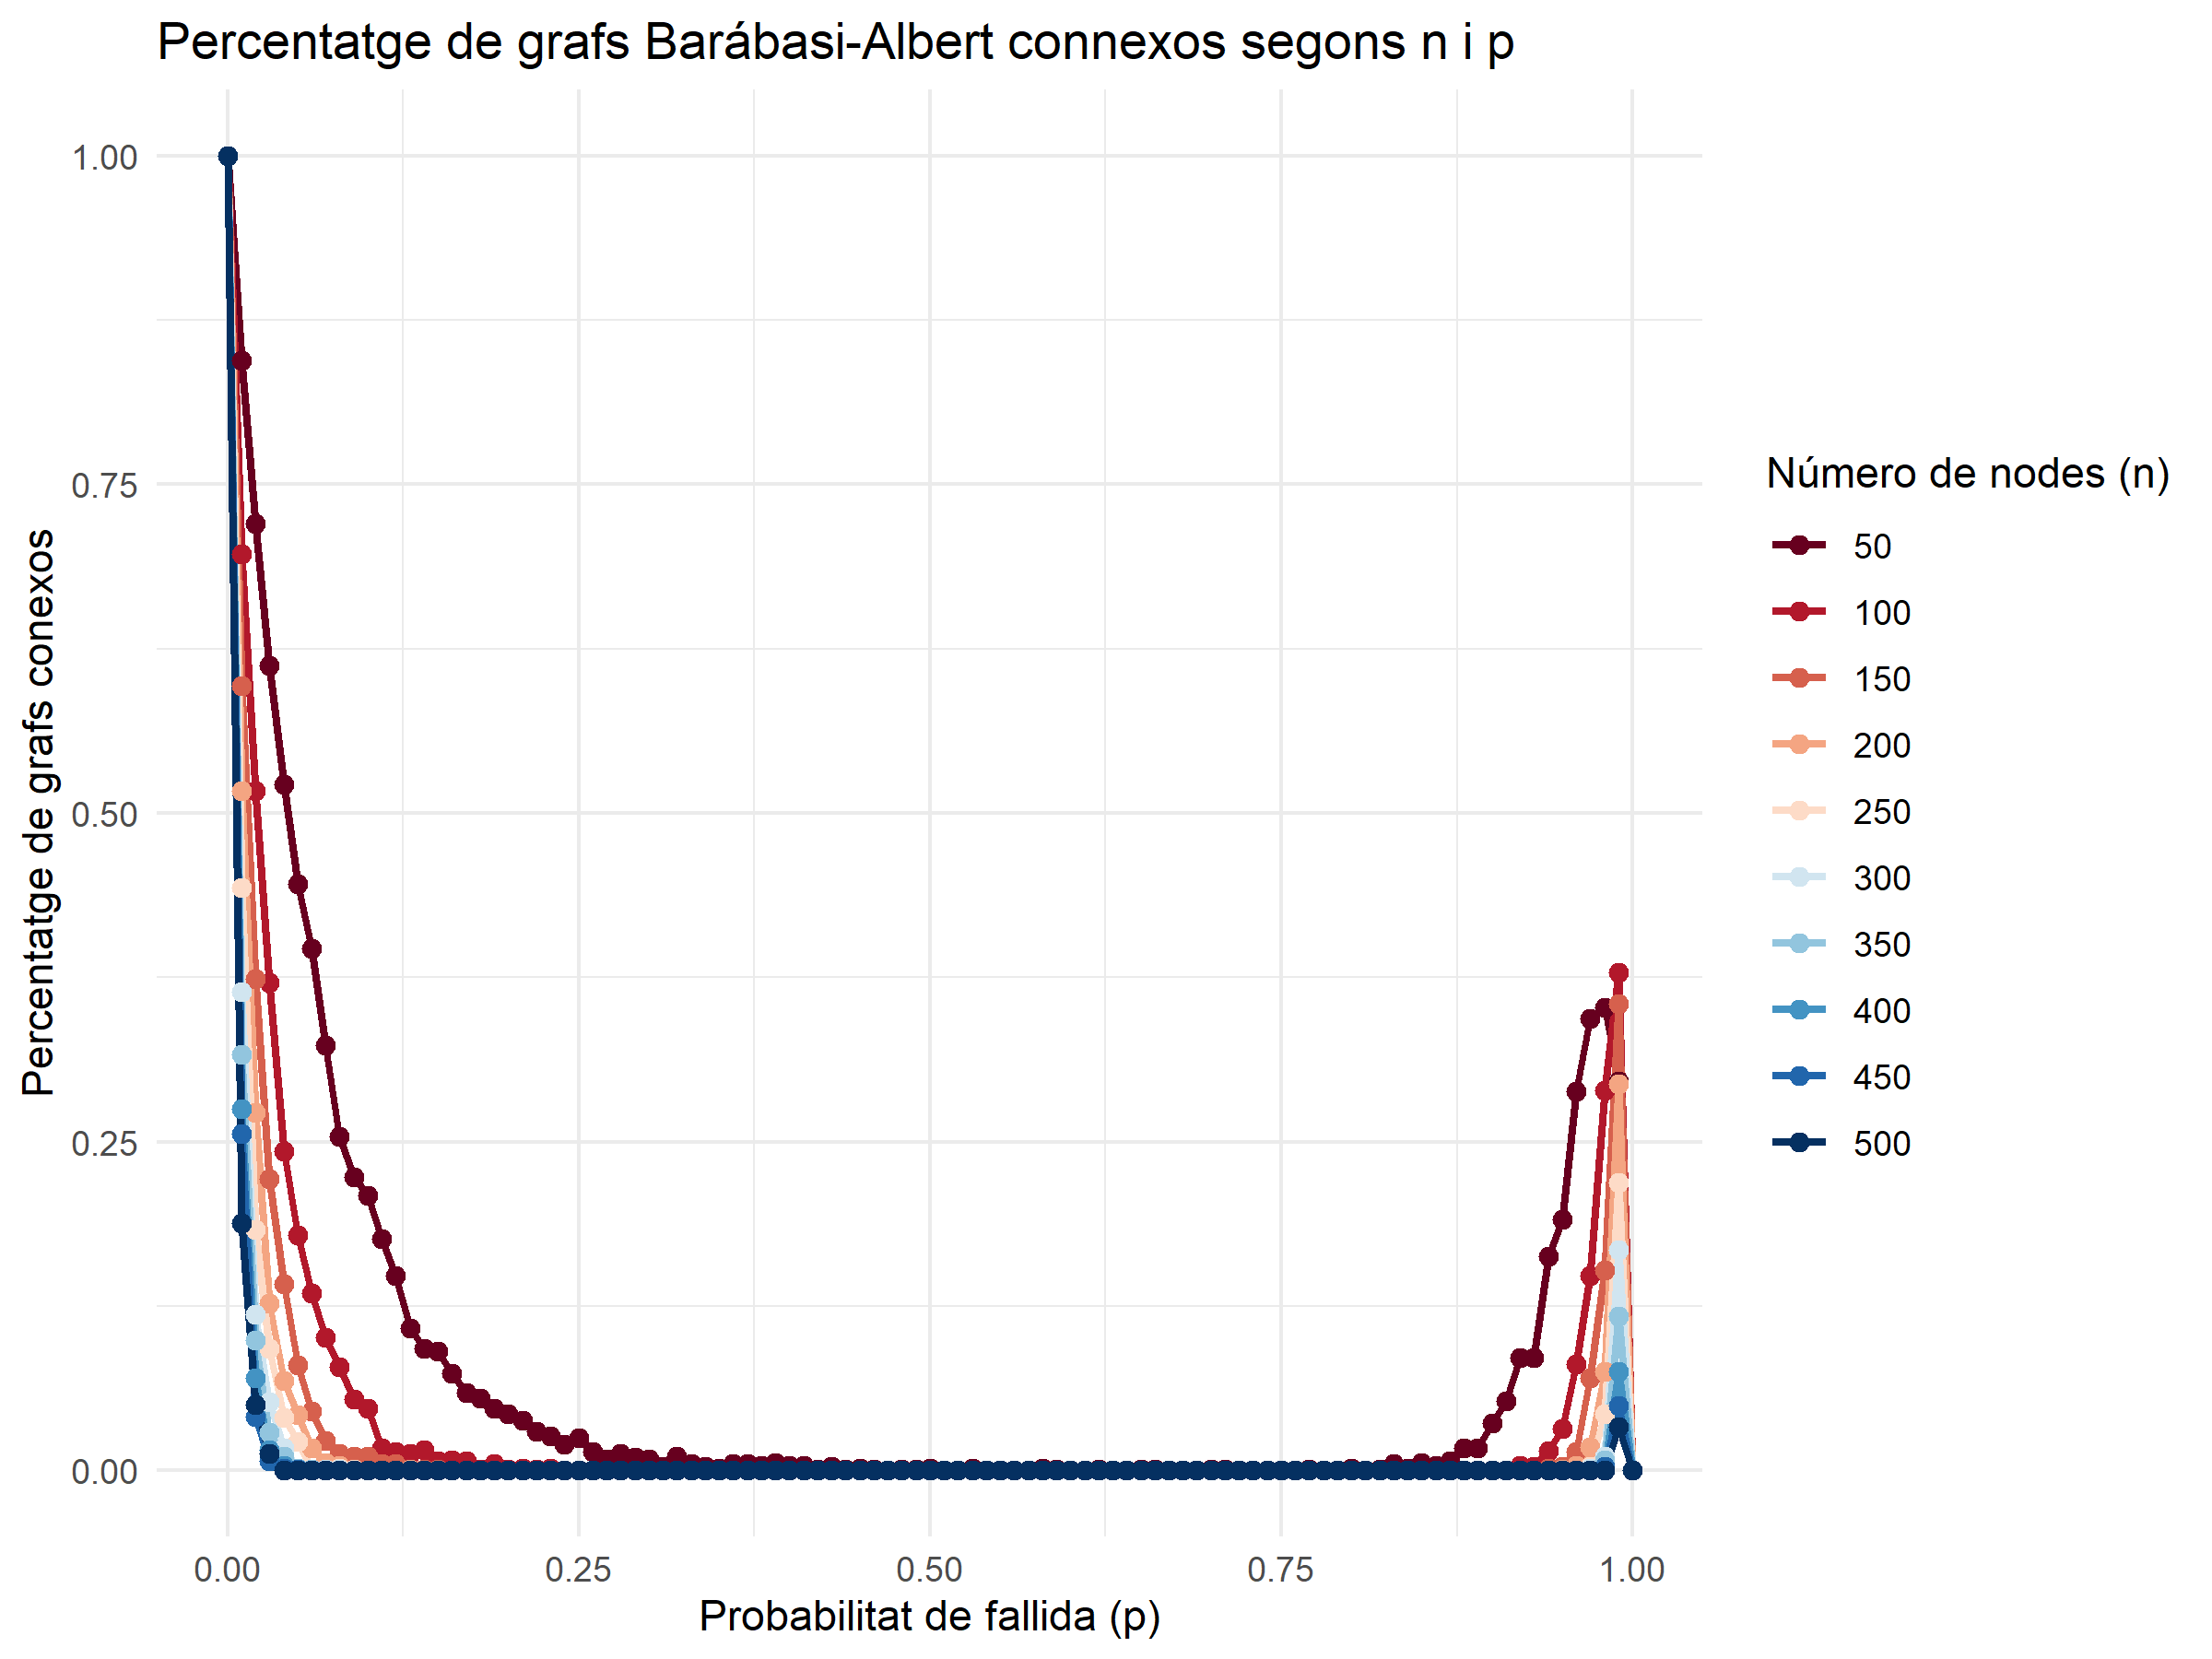
\includegraphics[width=\textwidth]{images/barabasi_50-500_2_1}
			\footnotesize{7673658 50 500 50 1000 NODE\_PERC ./data/ba13.csv Barabasi-Albert 2 1}
		\end{minipage}
		\caption{Comparativa de percolació per arestes del grafs Barabási-Albert amb $n$ = 10..100 (1) i $n$ = 50..500 (2), $m0$ = 2, $m$ = 1}
		\label{fig:percolation_nodes_ba_2_1}
	\end{figure}
	
	\begin{figure}[H]
		\centering
		\begin{minipage}{0.45\textwidth}
			\centering
			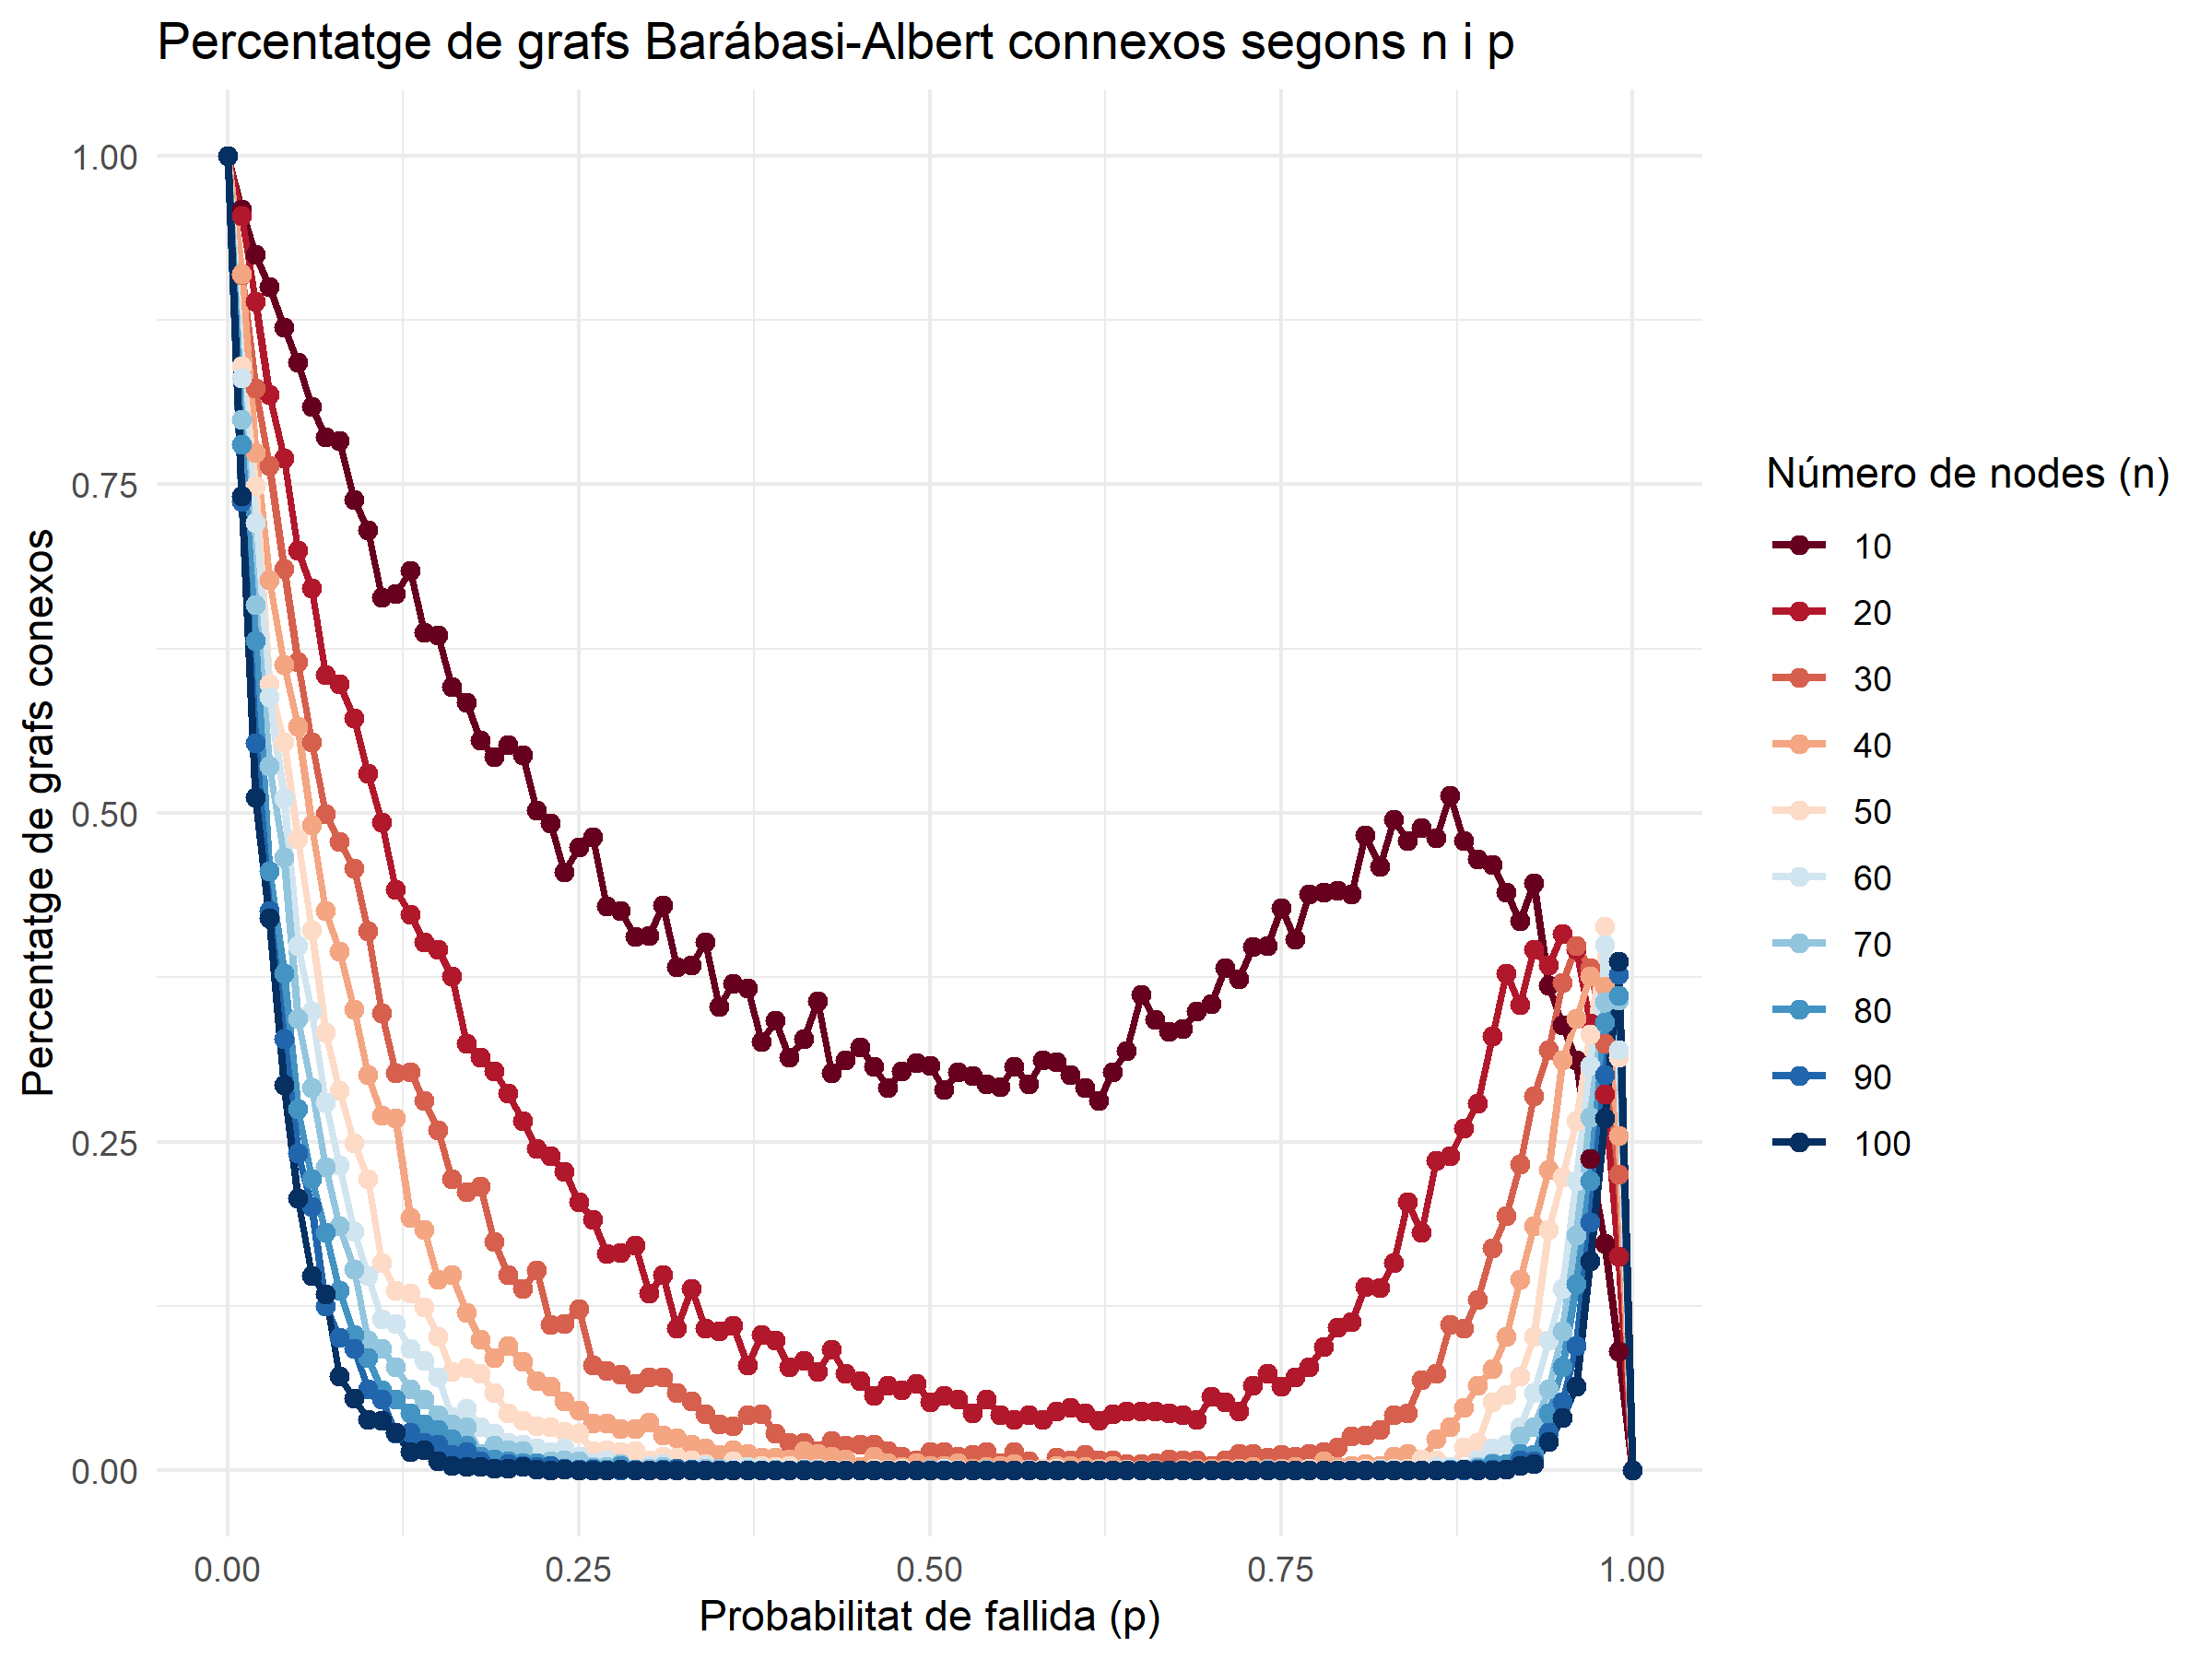
\includegraphics[width=\textwidth]{images/barabasi_10-100_5_1}
			\footnotesize{9937843 10 100 10 1000 NODE\_PERC ./data/ba10.csv Barabasi-Albert 5 1}
		\end{minipage}
		\hfill
		\begin{minipage}{0.45\textwidth}
			\centering
			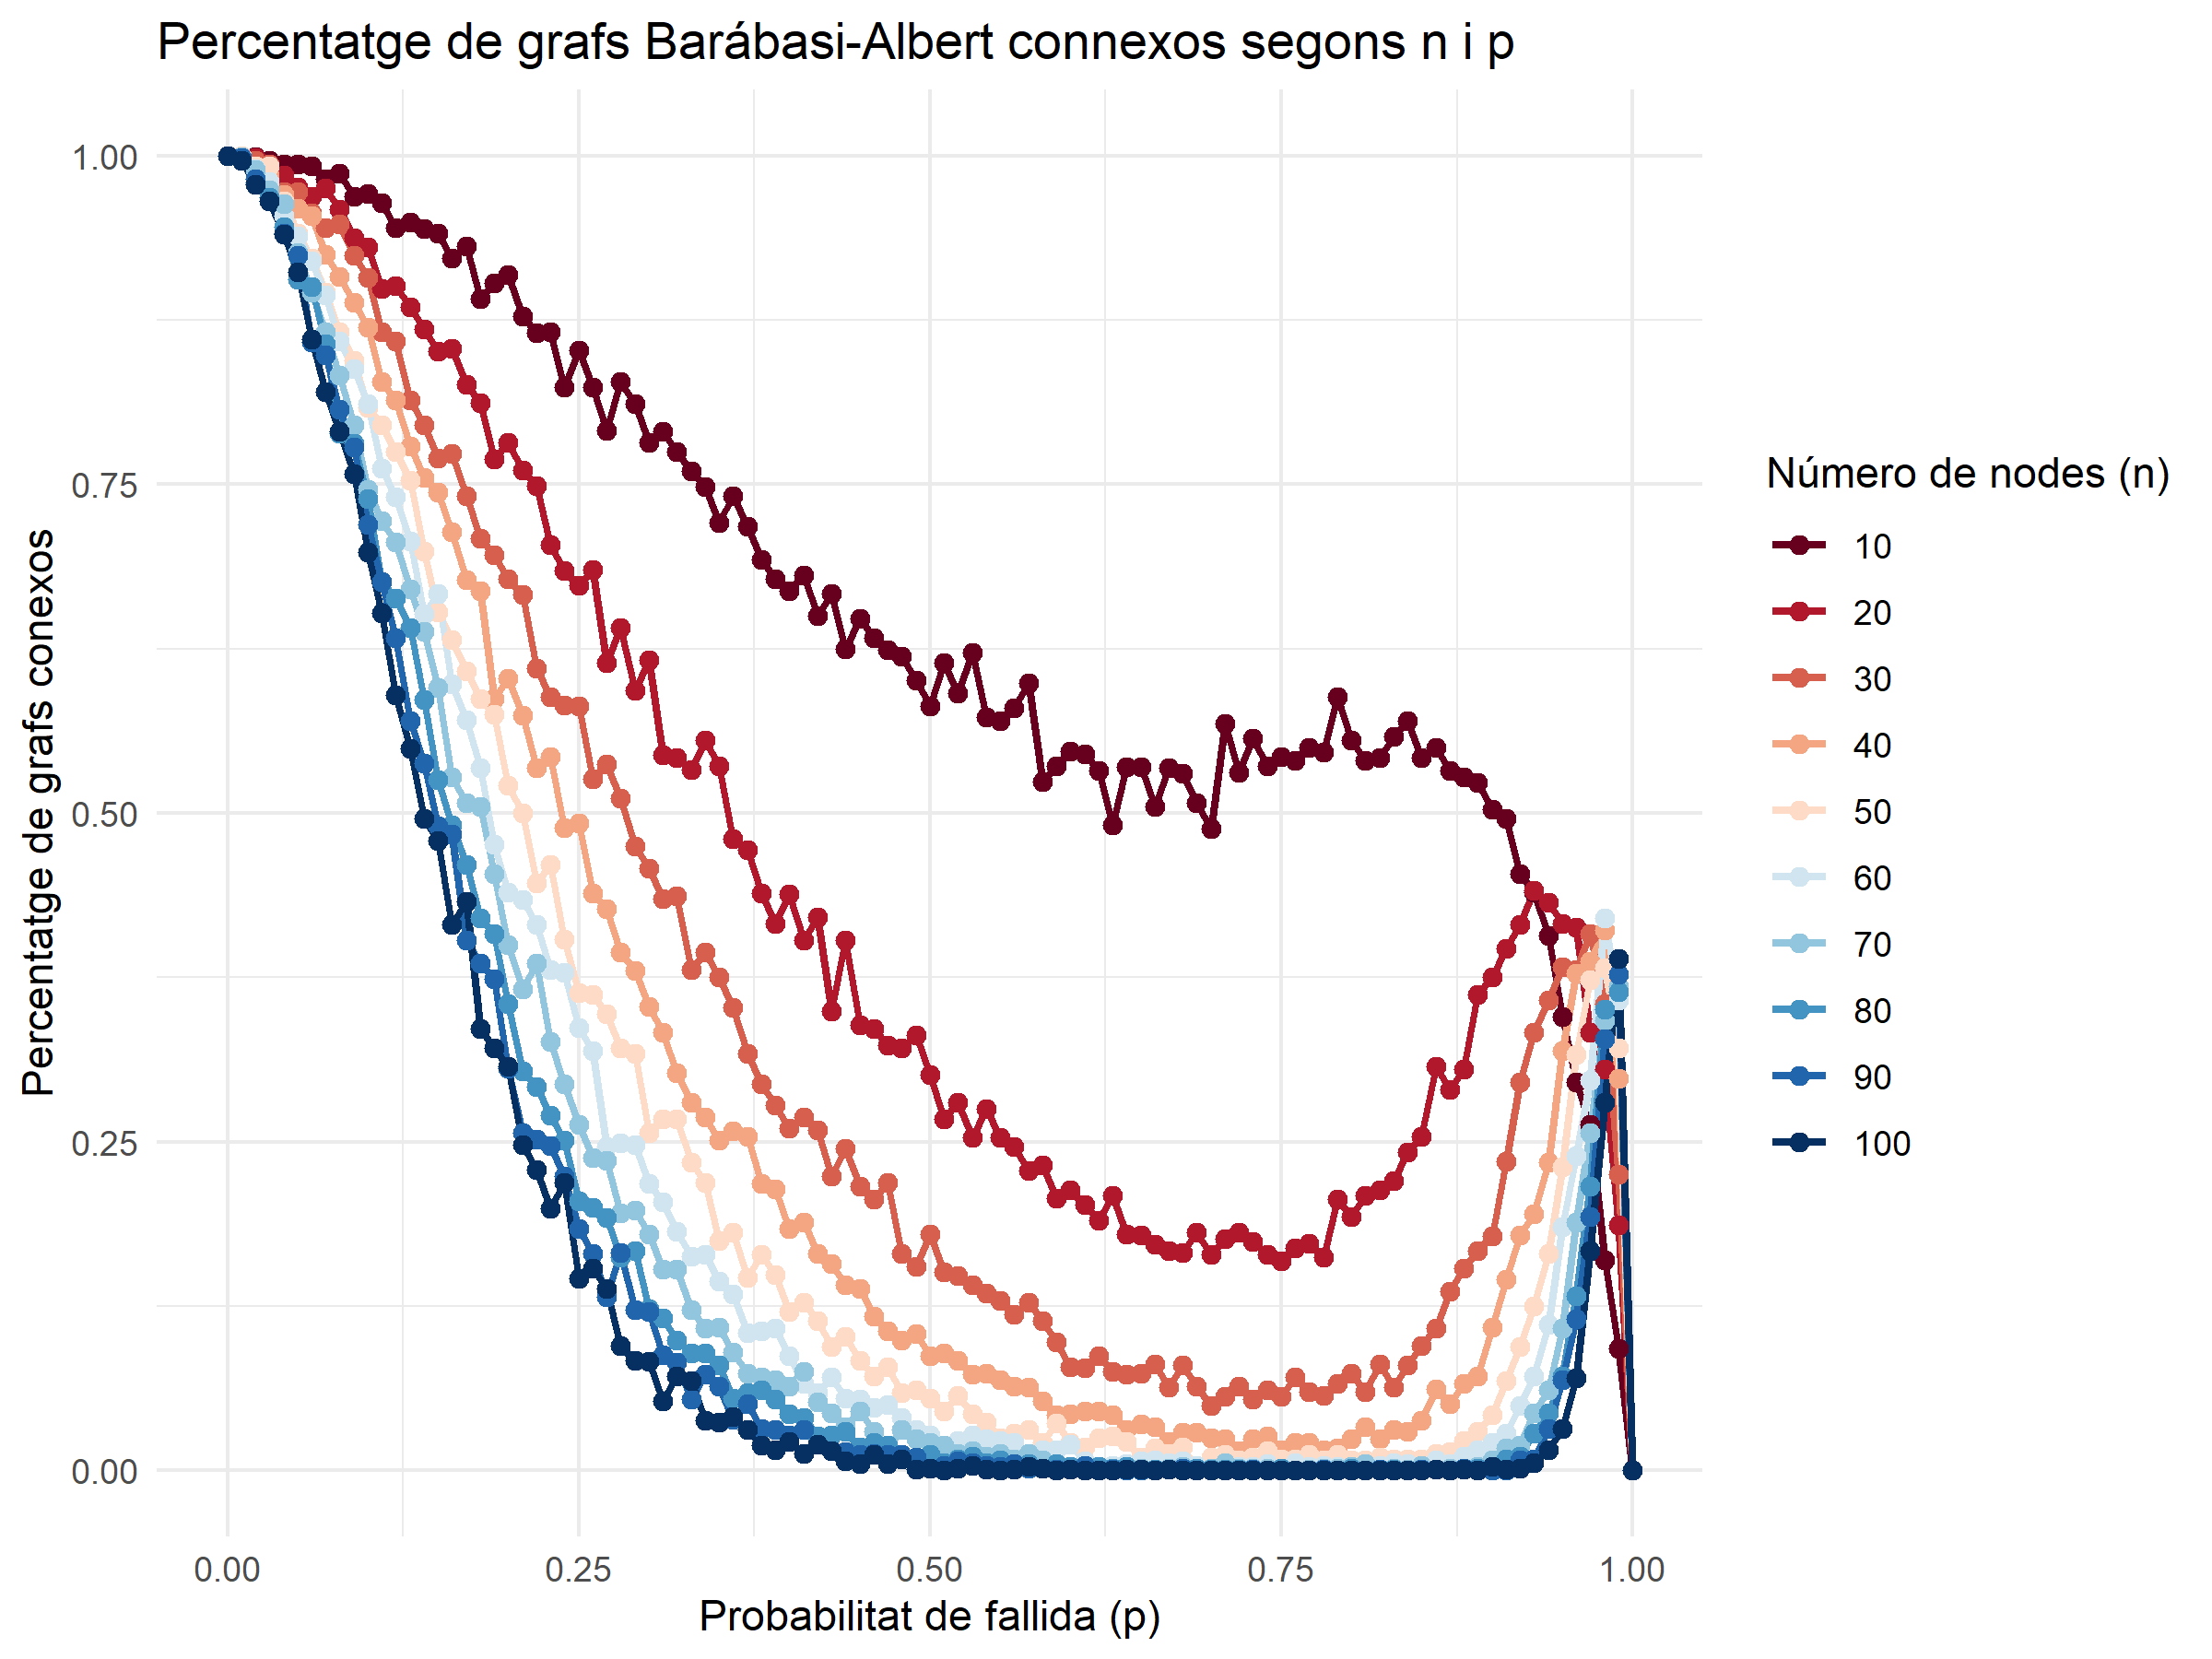
\includegraphics[width=\textwidth]{images/barabasi_10-100_5_2}
			\footnotesize{8800547 10 100 10 1000 NODE\_PERC ./data/ba11.csv Barabasi-Albert 5 2}
		\end{minipage}
		\caption{Comparativa de percolació per arestes del grafs Barabási-Albert amb $n$ = 10..100, $m0$ = 5, $m$ = 1 (1) i $m$ = 2 (2)}
		\label{fig:percolation_nodes_ba_5_x}
	\end{figure}
	
	\begin{figure}[H]
		\centering
		\begin{minipage}{0.45\textwidth}
			\centering
			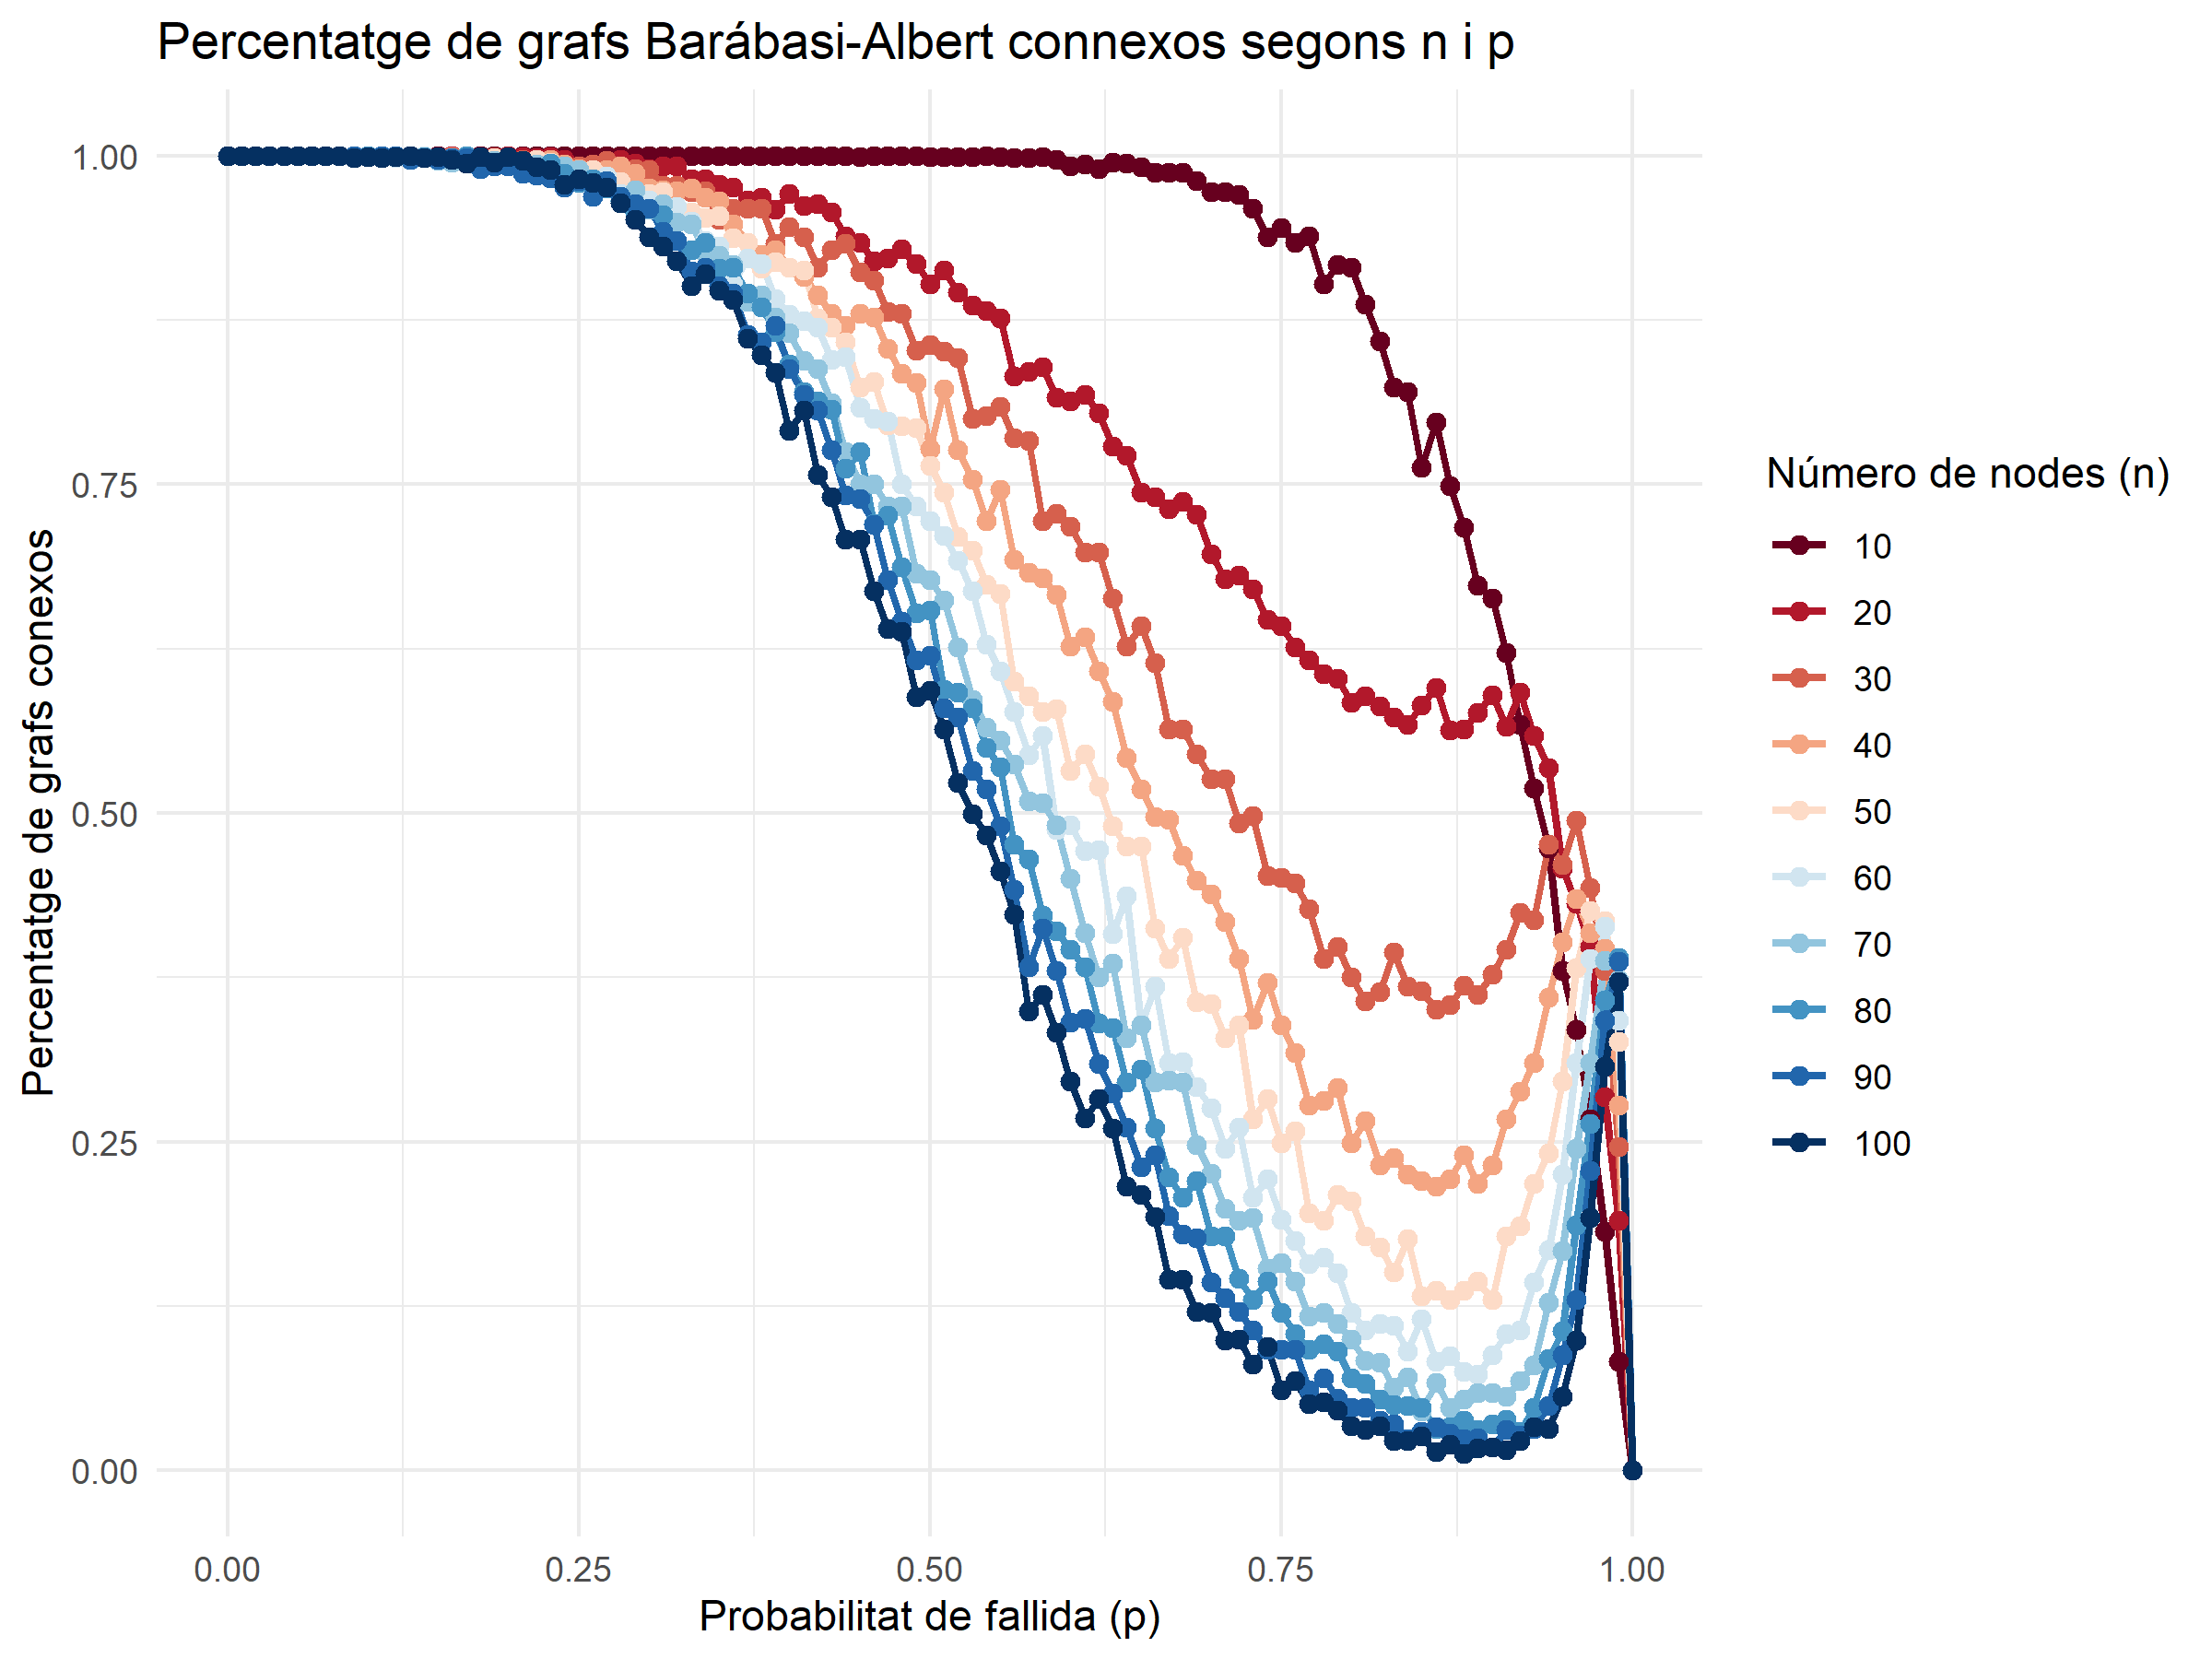
\includegraphics[width=\textwidth]{images/barabasi_10-100_10_5}
			\footnotesize{6657323 10 100 10 1000 NODE\_PERC ./data/ba15.csv Barabasi-Albert 10 5}
		\end{minipage}
		\hfill
		\begin{minipage}{0.45\textwidth}
			\centering
			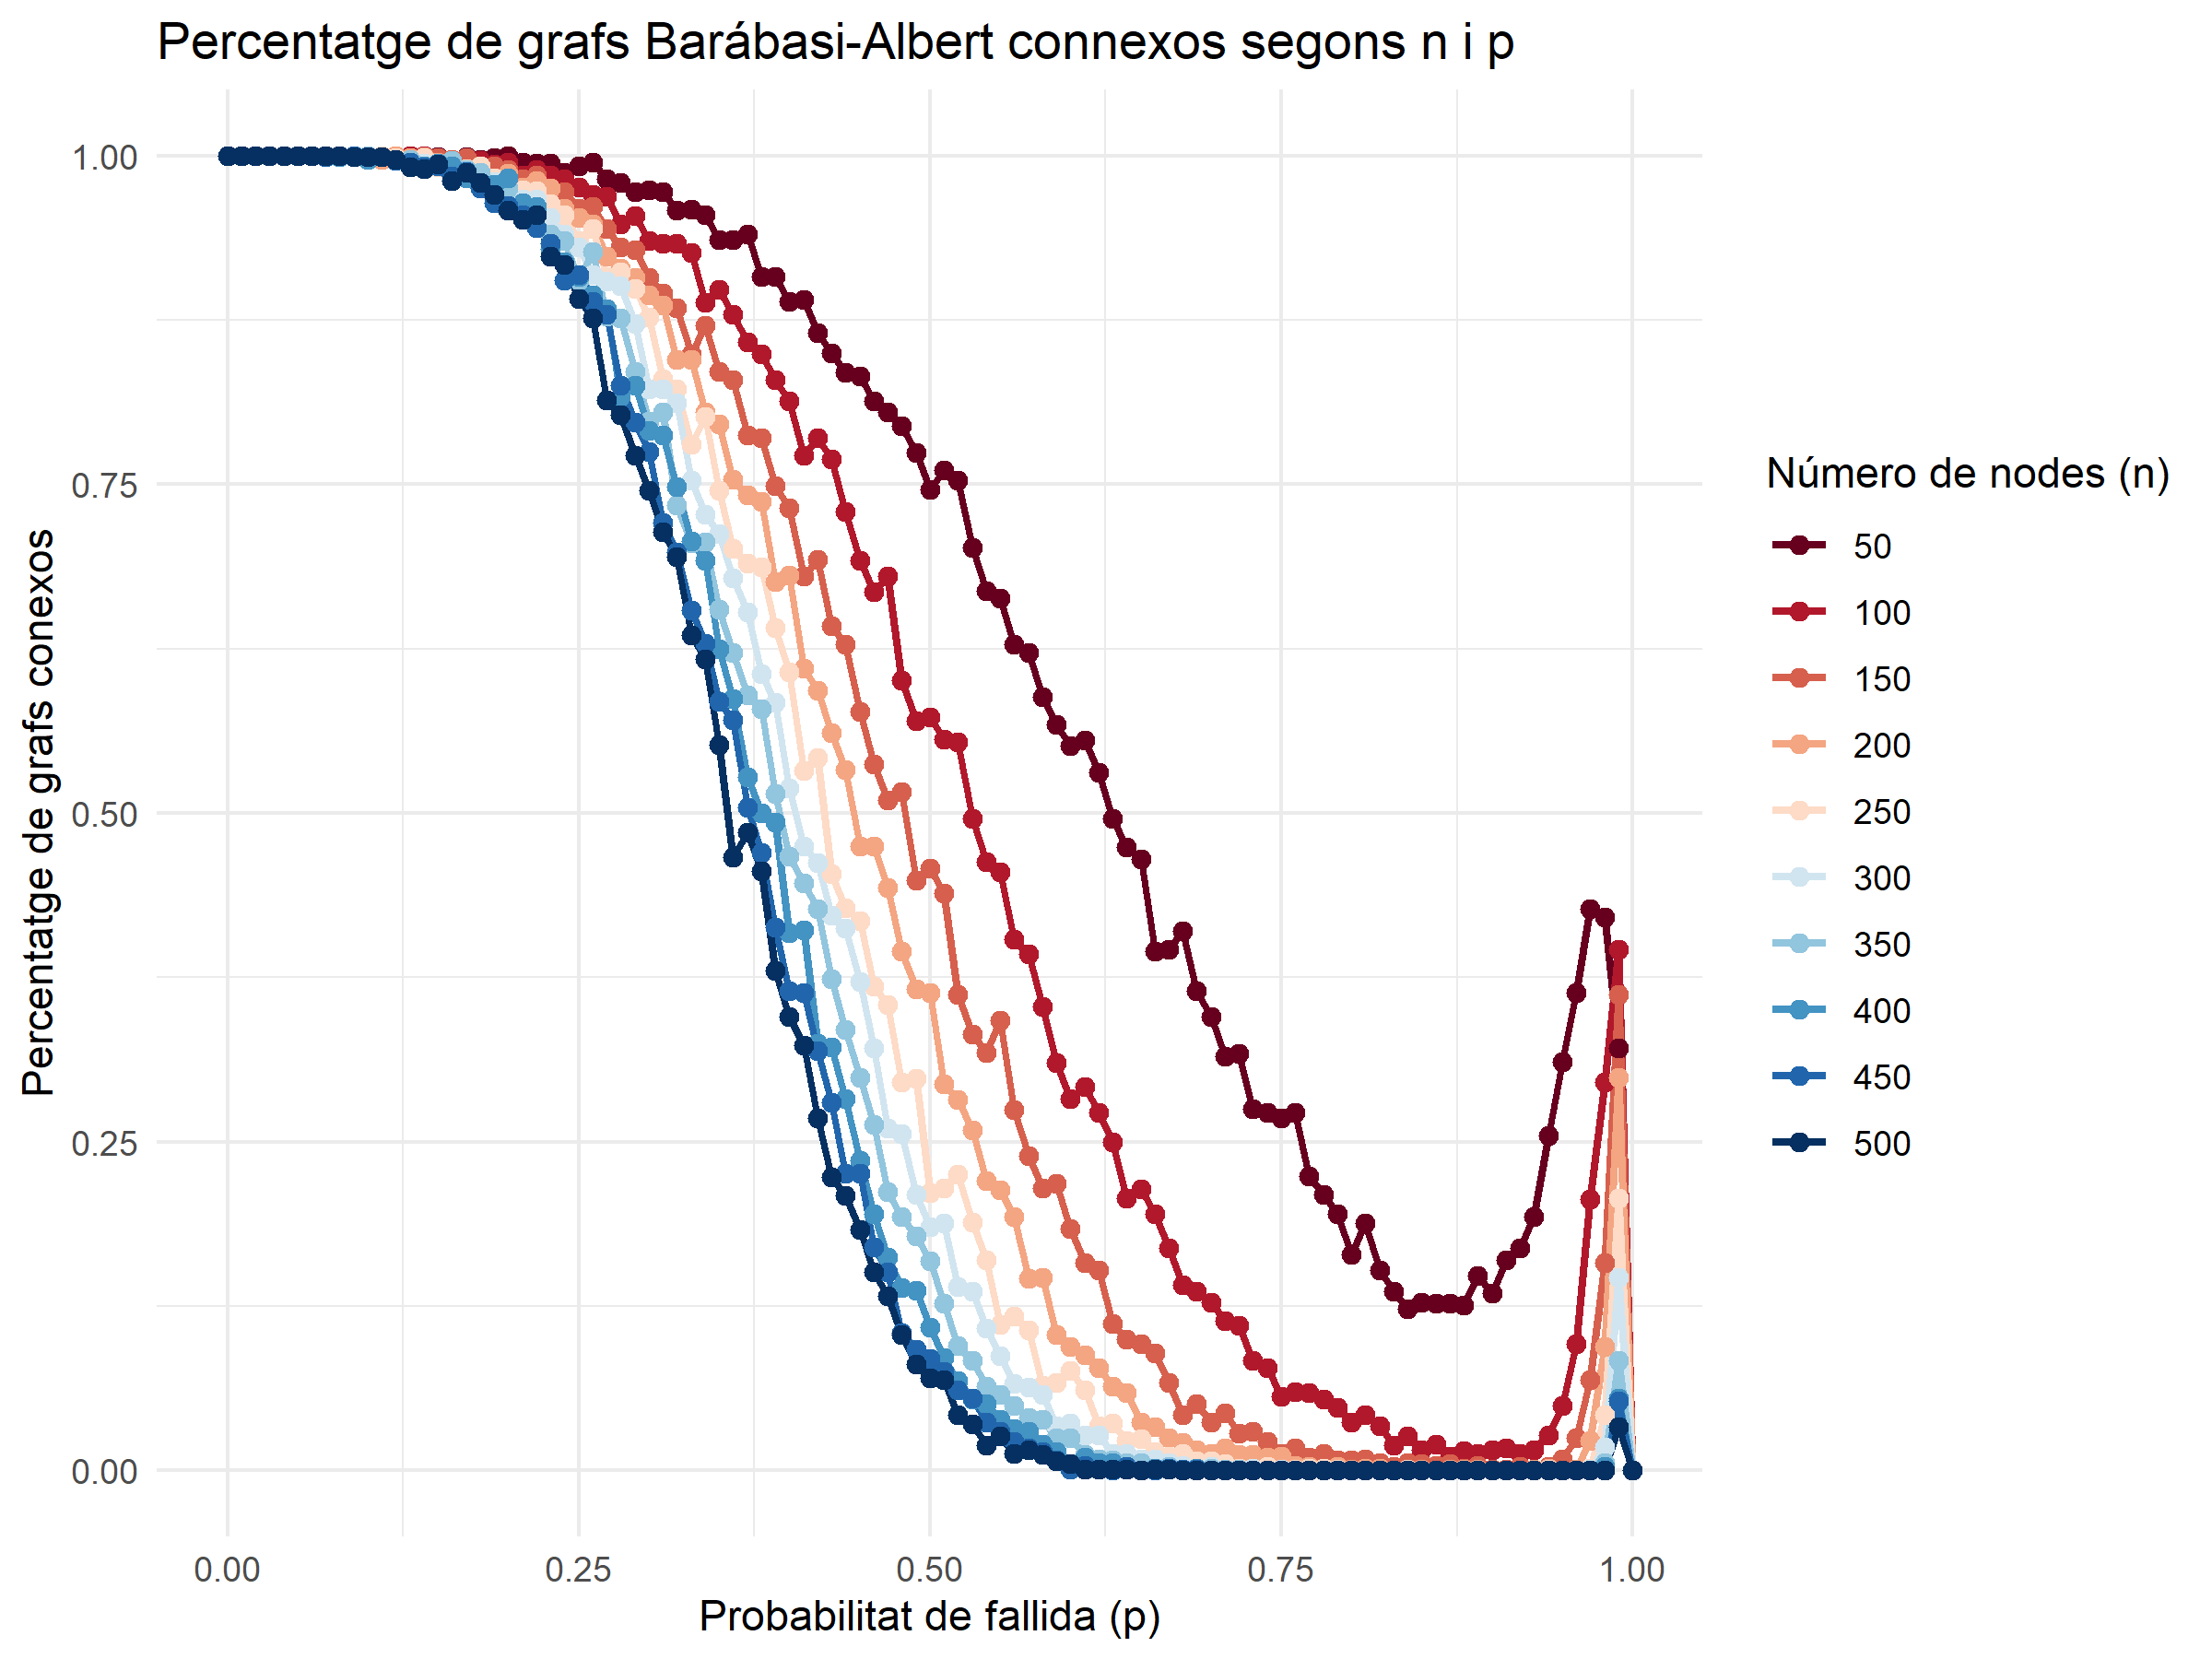
\includegraphics[width=\textwidth]{images/barabasi_50-500_10_5}
			\footnotesize{9872345 50 500 50 1000 NODE\_PERC ./data/ba16.csv Barabasi-Albert 10 5}
		\end{minipage}
		\caption{Comparativa de percolació per arestes del grafs Barabási-Albert amb $n$ = 10..100 (1) i $n$ = 50..500 (2), $m0$ = 10 $m$ = 5}
		\label{fig:percolation_nodes_ba_10_x}
	\end{figure}
		
	\newpage	
	\section{Conclusions}
	
	En aquest estudi, hem explorat els efectes de la percolació en diversos models de grafs, analitzant com la probabilitat de fallada i el nombre de nodes afecten la seva connectivitat i com es produeix la transició de fase. Els models seleccionats inclouen la graella quadrada, la graella triangular, els grafs geomètrics aleatoris i el model de Barabási-Albert. Hem aplicat tant percolació per arestes com per nodes, observant com varien els resultats en funció de la mida i estructura del graf. \\
	
	Els resultats obtinguts mostren patrons clars: a mesura que augmenta el nombre de nodes, la transició de fase esdevé més abrupta i ocorre amb valors més petits de probabilitat de fallida. Això és especialment evident en grafs més densos, com les graelles triangulars i els grafs geomètrics amb un radi de connexió gran, on la desconnexió completa es retarda. En canvi, en el model de Barabási-Albert, la percolació afecta més ràpidament la connectivitat quan fallen els hubs, mostrant la fragilitat de les xarxes amb concentració de connexions. \\
	
	En futurs treballs, seria interessant ampliar l'estudi amb altres tipus de grafs, com els grafs Erdős-Rényi o els grafs dirigits, així com investigar a part de la connectivitat com a propietat booleana, el nombre de components connexes després del procés de percolació. A més, es podria explorar l'impacte de percolacions selectives o correlacionades, on la fallada d'un node o aresta depengui de la fallada dels seus veïns, per entendre millor les propietats de robustesa i vulnerabilitat de les xarxes complexes.
	
	\newpage
	\section{Bibliografia}
	\renewcommand{\refname}{}	
	\begin{thebibliography}{99}
		\vspace{-2em}
		\bibitem{site_percolation} E. Weisstein, "Site Percolation", \textit{MathWorld -- A Wolfram Web Resource}. Disponible: \href{https://mathworld.wolfram.com/SitePercolation.html}{https://mathworld.wolfram.com/SitePercolation.html}. [Accedit: 17-oct-2024].
		
		\bibitem{bond_percolation} E. Weisstein, "Bond Percolation", \textit{MathWorld -- A Wolfram Web Resource}. Disponible: \href{https://mathworld.wolfram.com/BondPercolation.html}{https://mathworld.wolfram.com/BondPercolation.html}. [Accedit: 17-oct-2024].

		\bibitem{grimmett} G. R. Grimmett i A. M. Stacey, "CRITICAL PROBABILITIES FOR SITE
		AND BOND PERCOLATION MODELS", Disponible: \href{http://www.statslab.cam.ac.uk/~grg1000/papers/UScrit6.pdf}{http://www.statslab.cam.ac.uk/~grg1000/papers/UScrit6.pdf}. [Accedit: 17-oct-2024].

	\end{thebibliography}
	
	
	\newpage
	\section{Annex}
	
	\end{document}